%chapter 8
\chapter{Data Analysis and Source Identification Techniques}
Laboratory tests on the MODES-SNM system were performed at a controlled environment at NCBJ in Poland. The collected data was the first that the prototype was exposed to and was used to characterise the system. Some studies are initially presented that were conducted by the collaboration members from NCBJ to quantify the basic properties of the detectors and examine the detector requirements. The chapter then focusses on the techniques employed to analyse the collected data, with the aim to discriminate between neutron and gamma sources for real world applications. This is an alternative analysis to the one implemented in the prototype and the one used in the live demonstrations, as it aims to improve on the existing analysis and to be implemented in future MODES-SNM like systems.

\section{Laboratory Characterisation}
Laboratory characterisation of the system was performed at NCBJ and the following section summarises the results of the work performed by the NCBJ contributors of the MODES-SNM project \cite{modesInternal}. The primary objective was to perform preliminary tests on the prototype system, specifically to assess the detectors response, efficiencies, resolutions and durability.

\subsection{Gamma Detector Response}
$^{137}$Cs (662 keV) and $^{241}$Am (59.6 keV) sources were introduced at 0.5 m from the centre of the xenon container to measure the detectors response. Figure \ref{fig:modesCs137Response} shows the xenon detector's response for the two sources, also compared to the background counts (no source). The signal amplitude is determined as the ADC counts measured in the long gate, corresponding to the $Q_{long}$ value from equation \ref{eq:modesPsdValue}. The non-linearity of this response is illustrated in figure \ref{fig:modesXenonNoLinearity}, it can be seen that the detectors energy response for gammas is no longer linear for energies less than $\sim$200 keV. This is due to increased scintillation efficiencies at these lower energies. Each point in figure \ref{fig:modesXenonNoLinearity} was determined from matching peaks in the signal amplitude to known energies from 9 different radioactive sources (14 peak energies between 50 keV and 1.5 MeV), using both channels on one of the xenon detectors. The measured peaks were normalised to that of the $^{137}$Cs source at 662 keV. The maximum linear deviation was observed at the 60 keV peak for which a measured difference of 8\% and 10\% for channels 0 and 1 respectively.

\begin{figure}[htbp]
\begin{center}
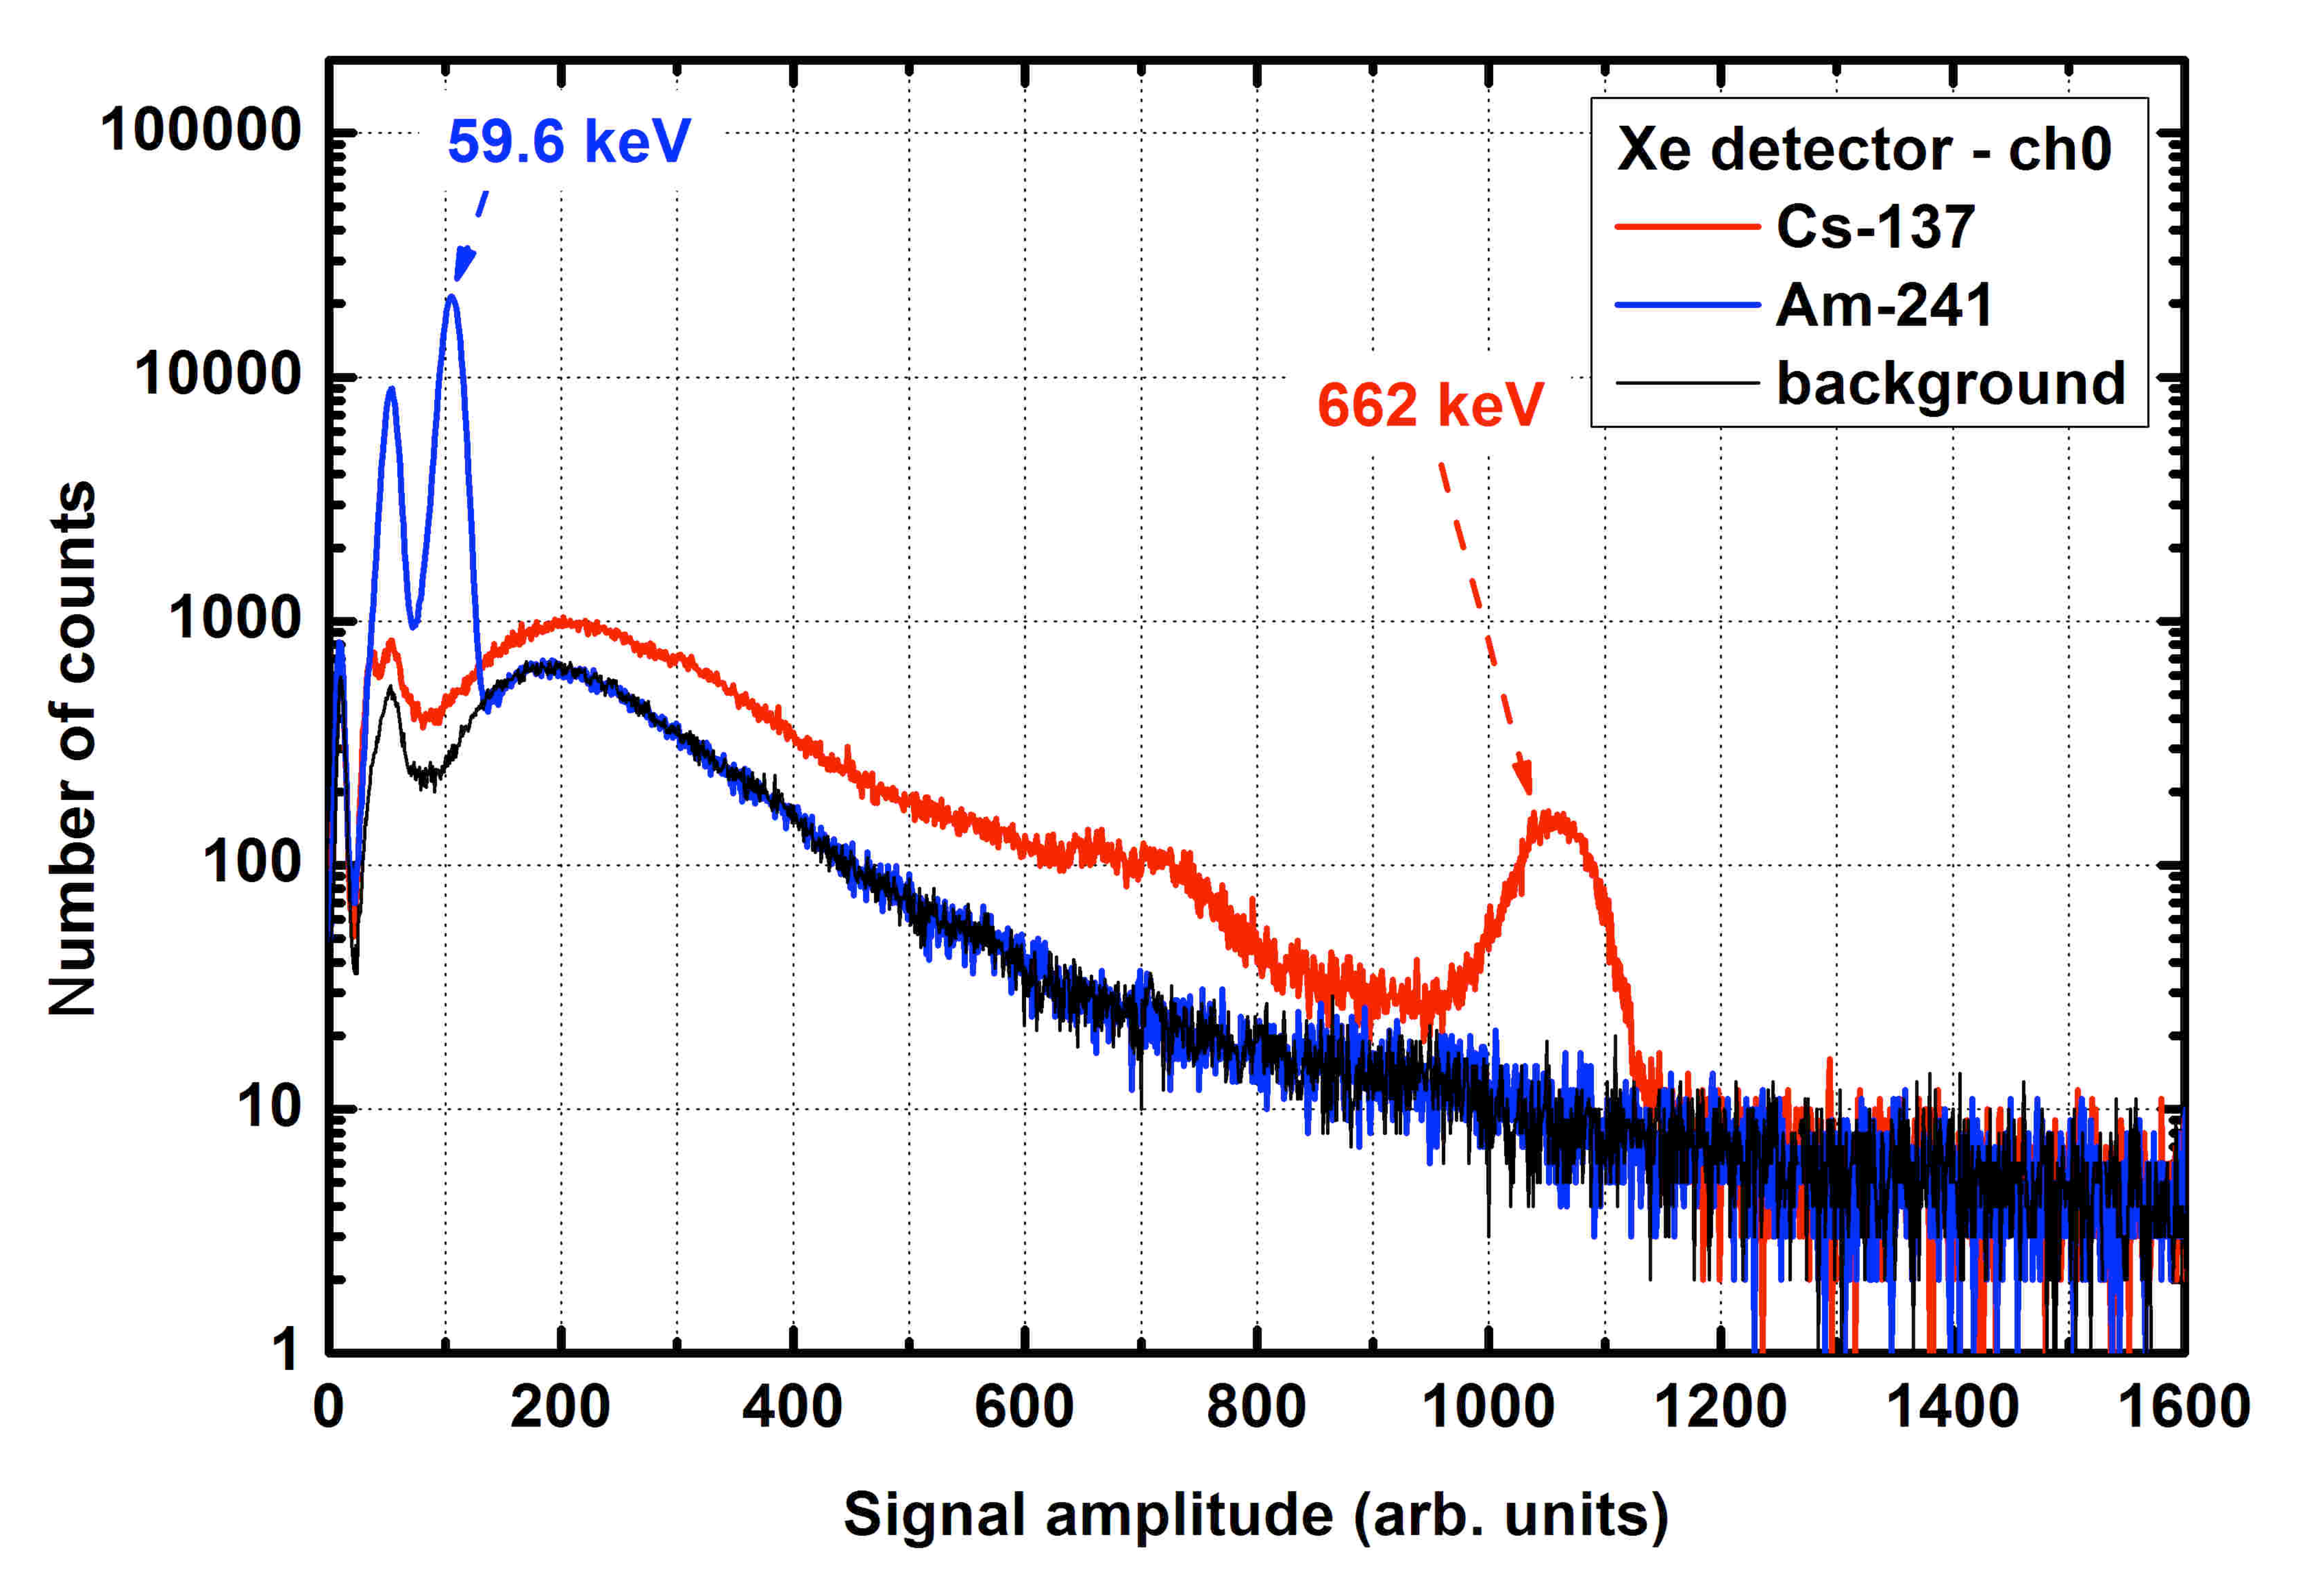
\includegraphics[width=100mm]{Chapter8/figures/Cs-137_XenonResponse.pdf}
\caption{The energy spectrum (signal amplitude) from one of the PMTs in the xenon detector for a $^{137}$Cs source (red line) and an $^{241}$Am source (blue line). The counts due to the absence of a nearby localised radioactive source is shown by the black line. Plot taken from \cite{modesInternal}.}
\label{fig:modesCs137Response}
\end{center}
\end{figure}

\begin{figure}[htbp]
\begin{center}
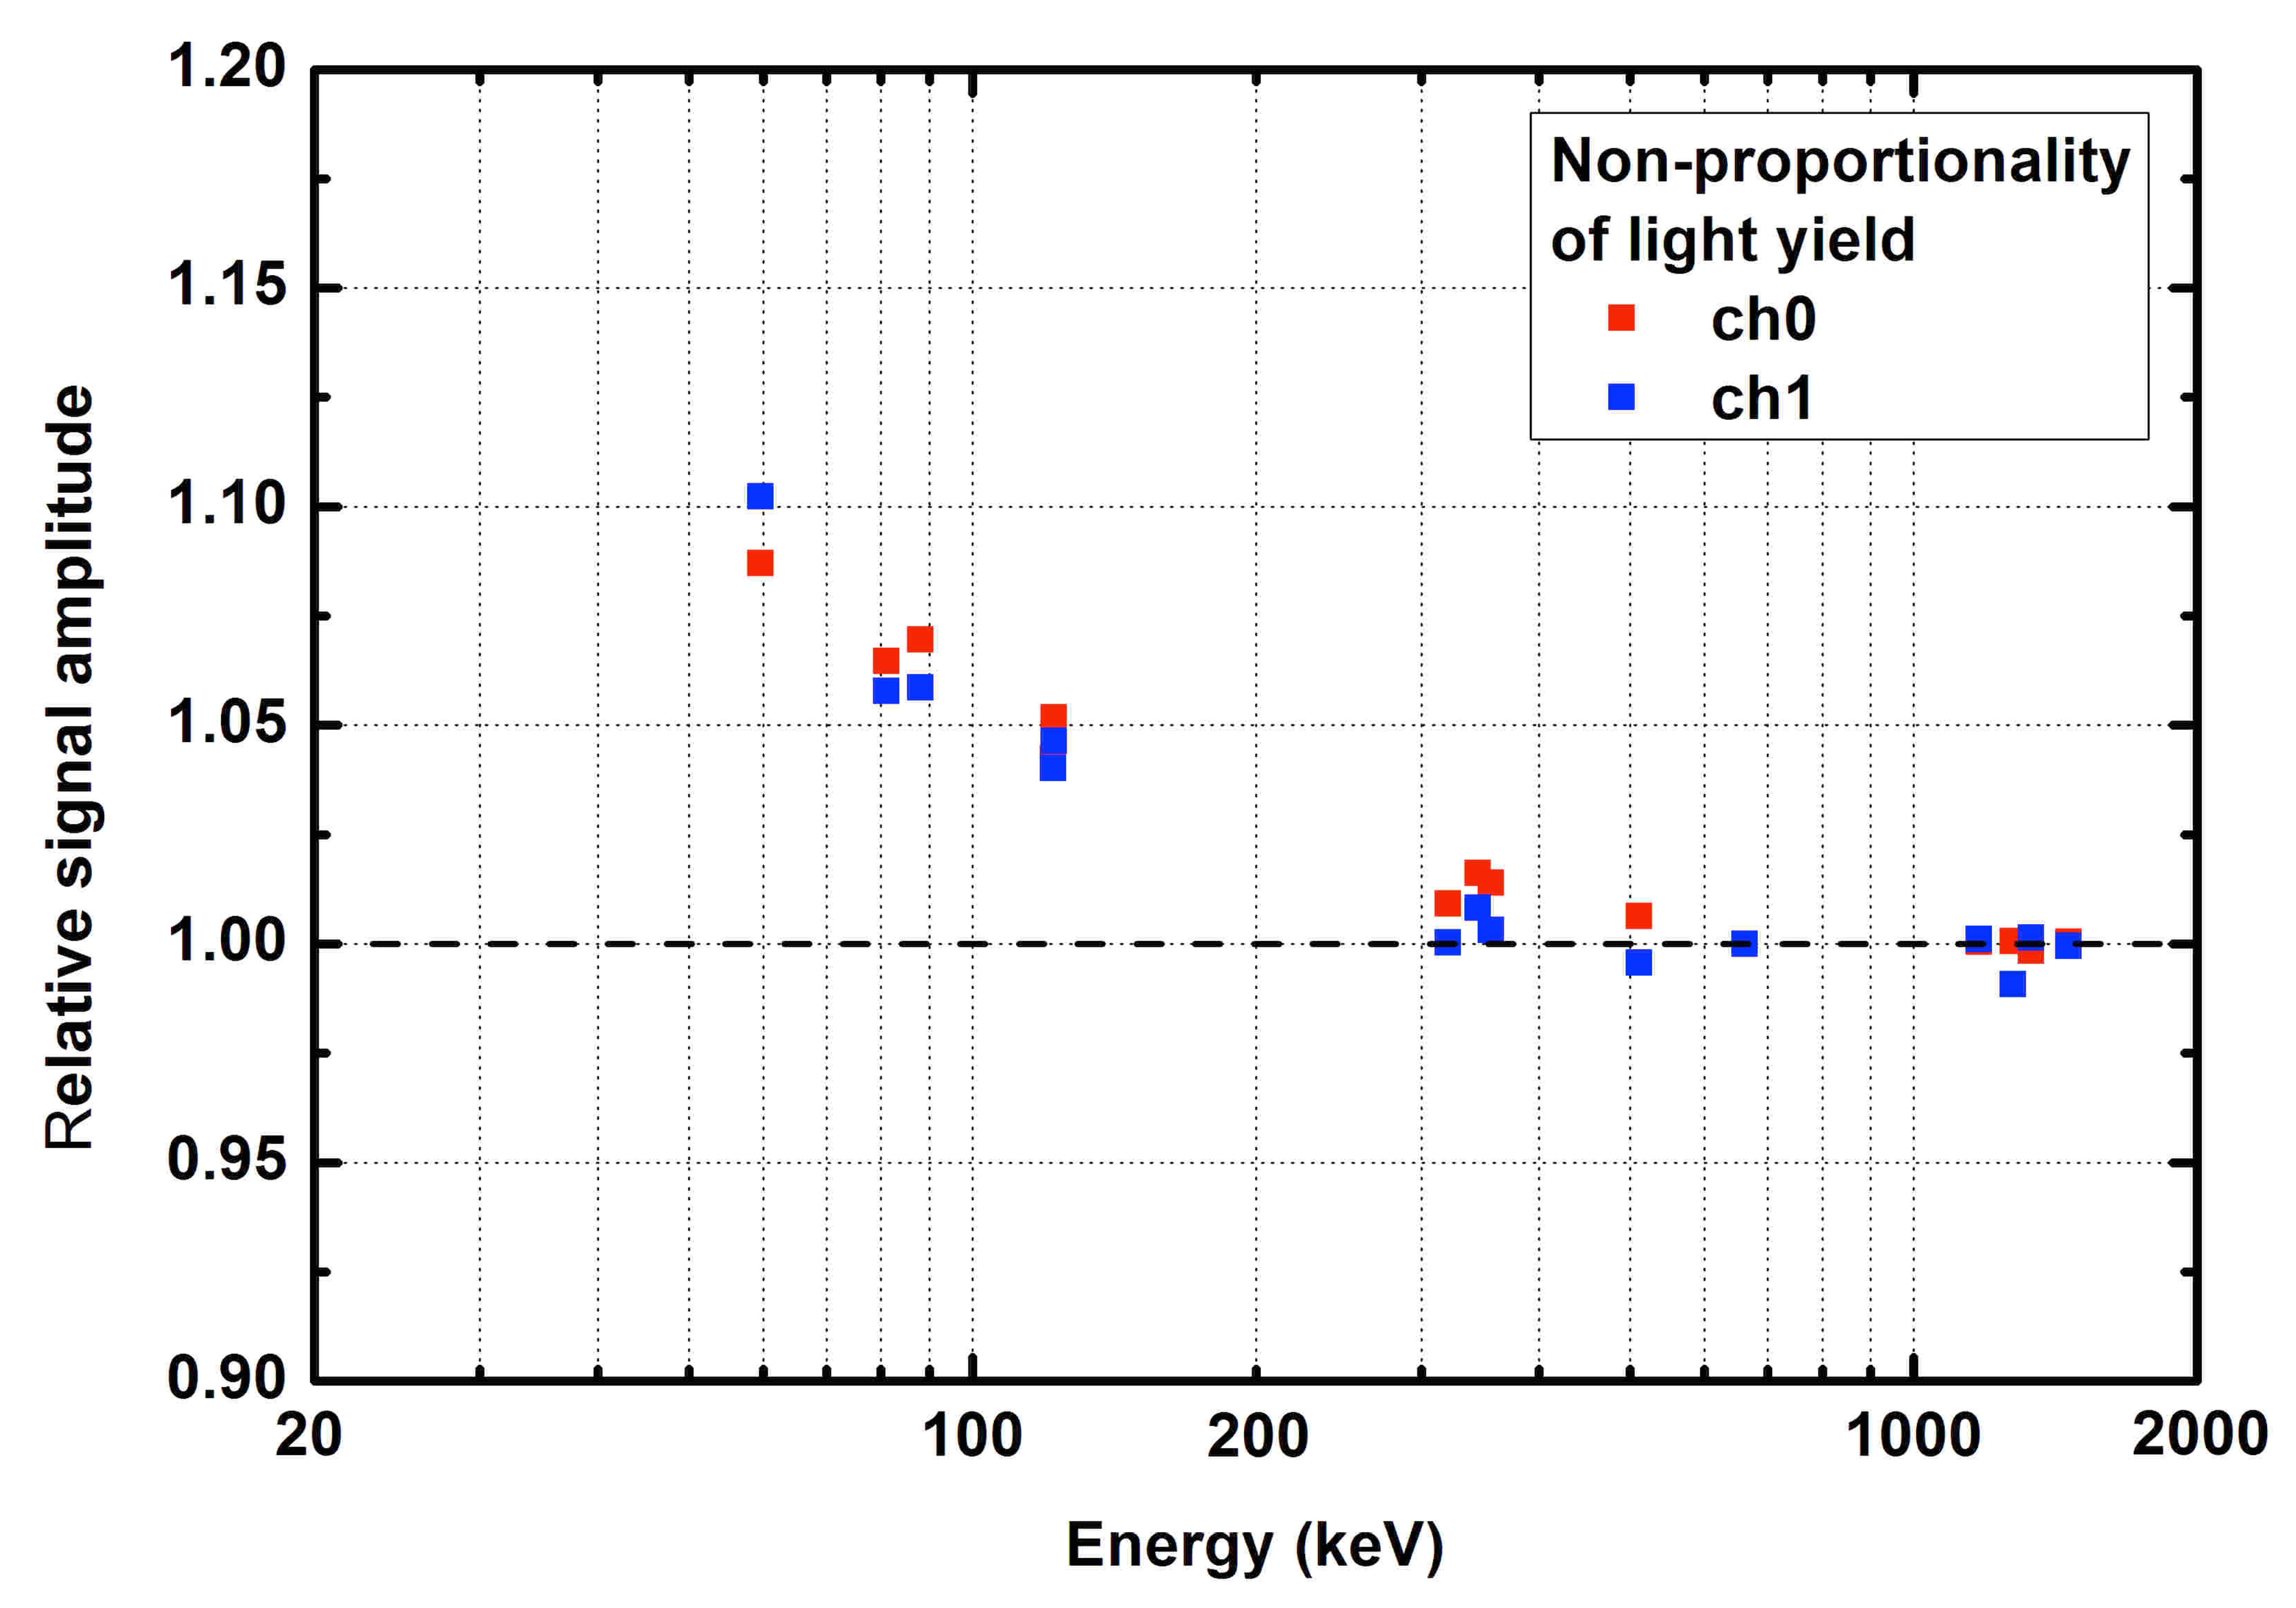
\includegraphics[width=100mm]{Chapter8/figures/XenonNonLinearity.pdf}
\caption{The relationship between the measured relative signal amplitude and the measured peak energy arising from several gamma sources. The signal amplitude is normalised to the 662 keV peak energy photon emission from a $^{137}$Cs source. Data points correspond to 14 measured energy peaks between 50 keV and 1.5 MeV for 9 known gamma sources, using both channels (channel 0 in red and channel 1 in blue) for one of the xenon detectors. Plot taken from \cite{modesInternal}.}
\label{fig:modesXenonNoLinearity}
\end{center}
\end{figure}

\subsubsection{Energy Resolution}
Defining the energy resolution as the FWHM (Full Width at Half Maximum) divided by the signal amplitude, measurements of the energy resolution for gammas in the xenon detector where established using the same 9 sources previously used for the linearity tests. Again only one of the xenon detectors was tested with both channels used. An energy resolution of between 6.7\% and 7.0\% \cite{modesInternal} was established for both channels on the detector at 662 keV, a value comparable to NaI detectors. The left of figure \ref{fig:modesXenonEnergyResolution} shows the energy resolution as a function of the source energy, showing resolutions less than 6\% for energies around 1.5 MeV but very poor resolutions for energies below 200 keV. 

\begin{figure}[htbp]
\begin{center}
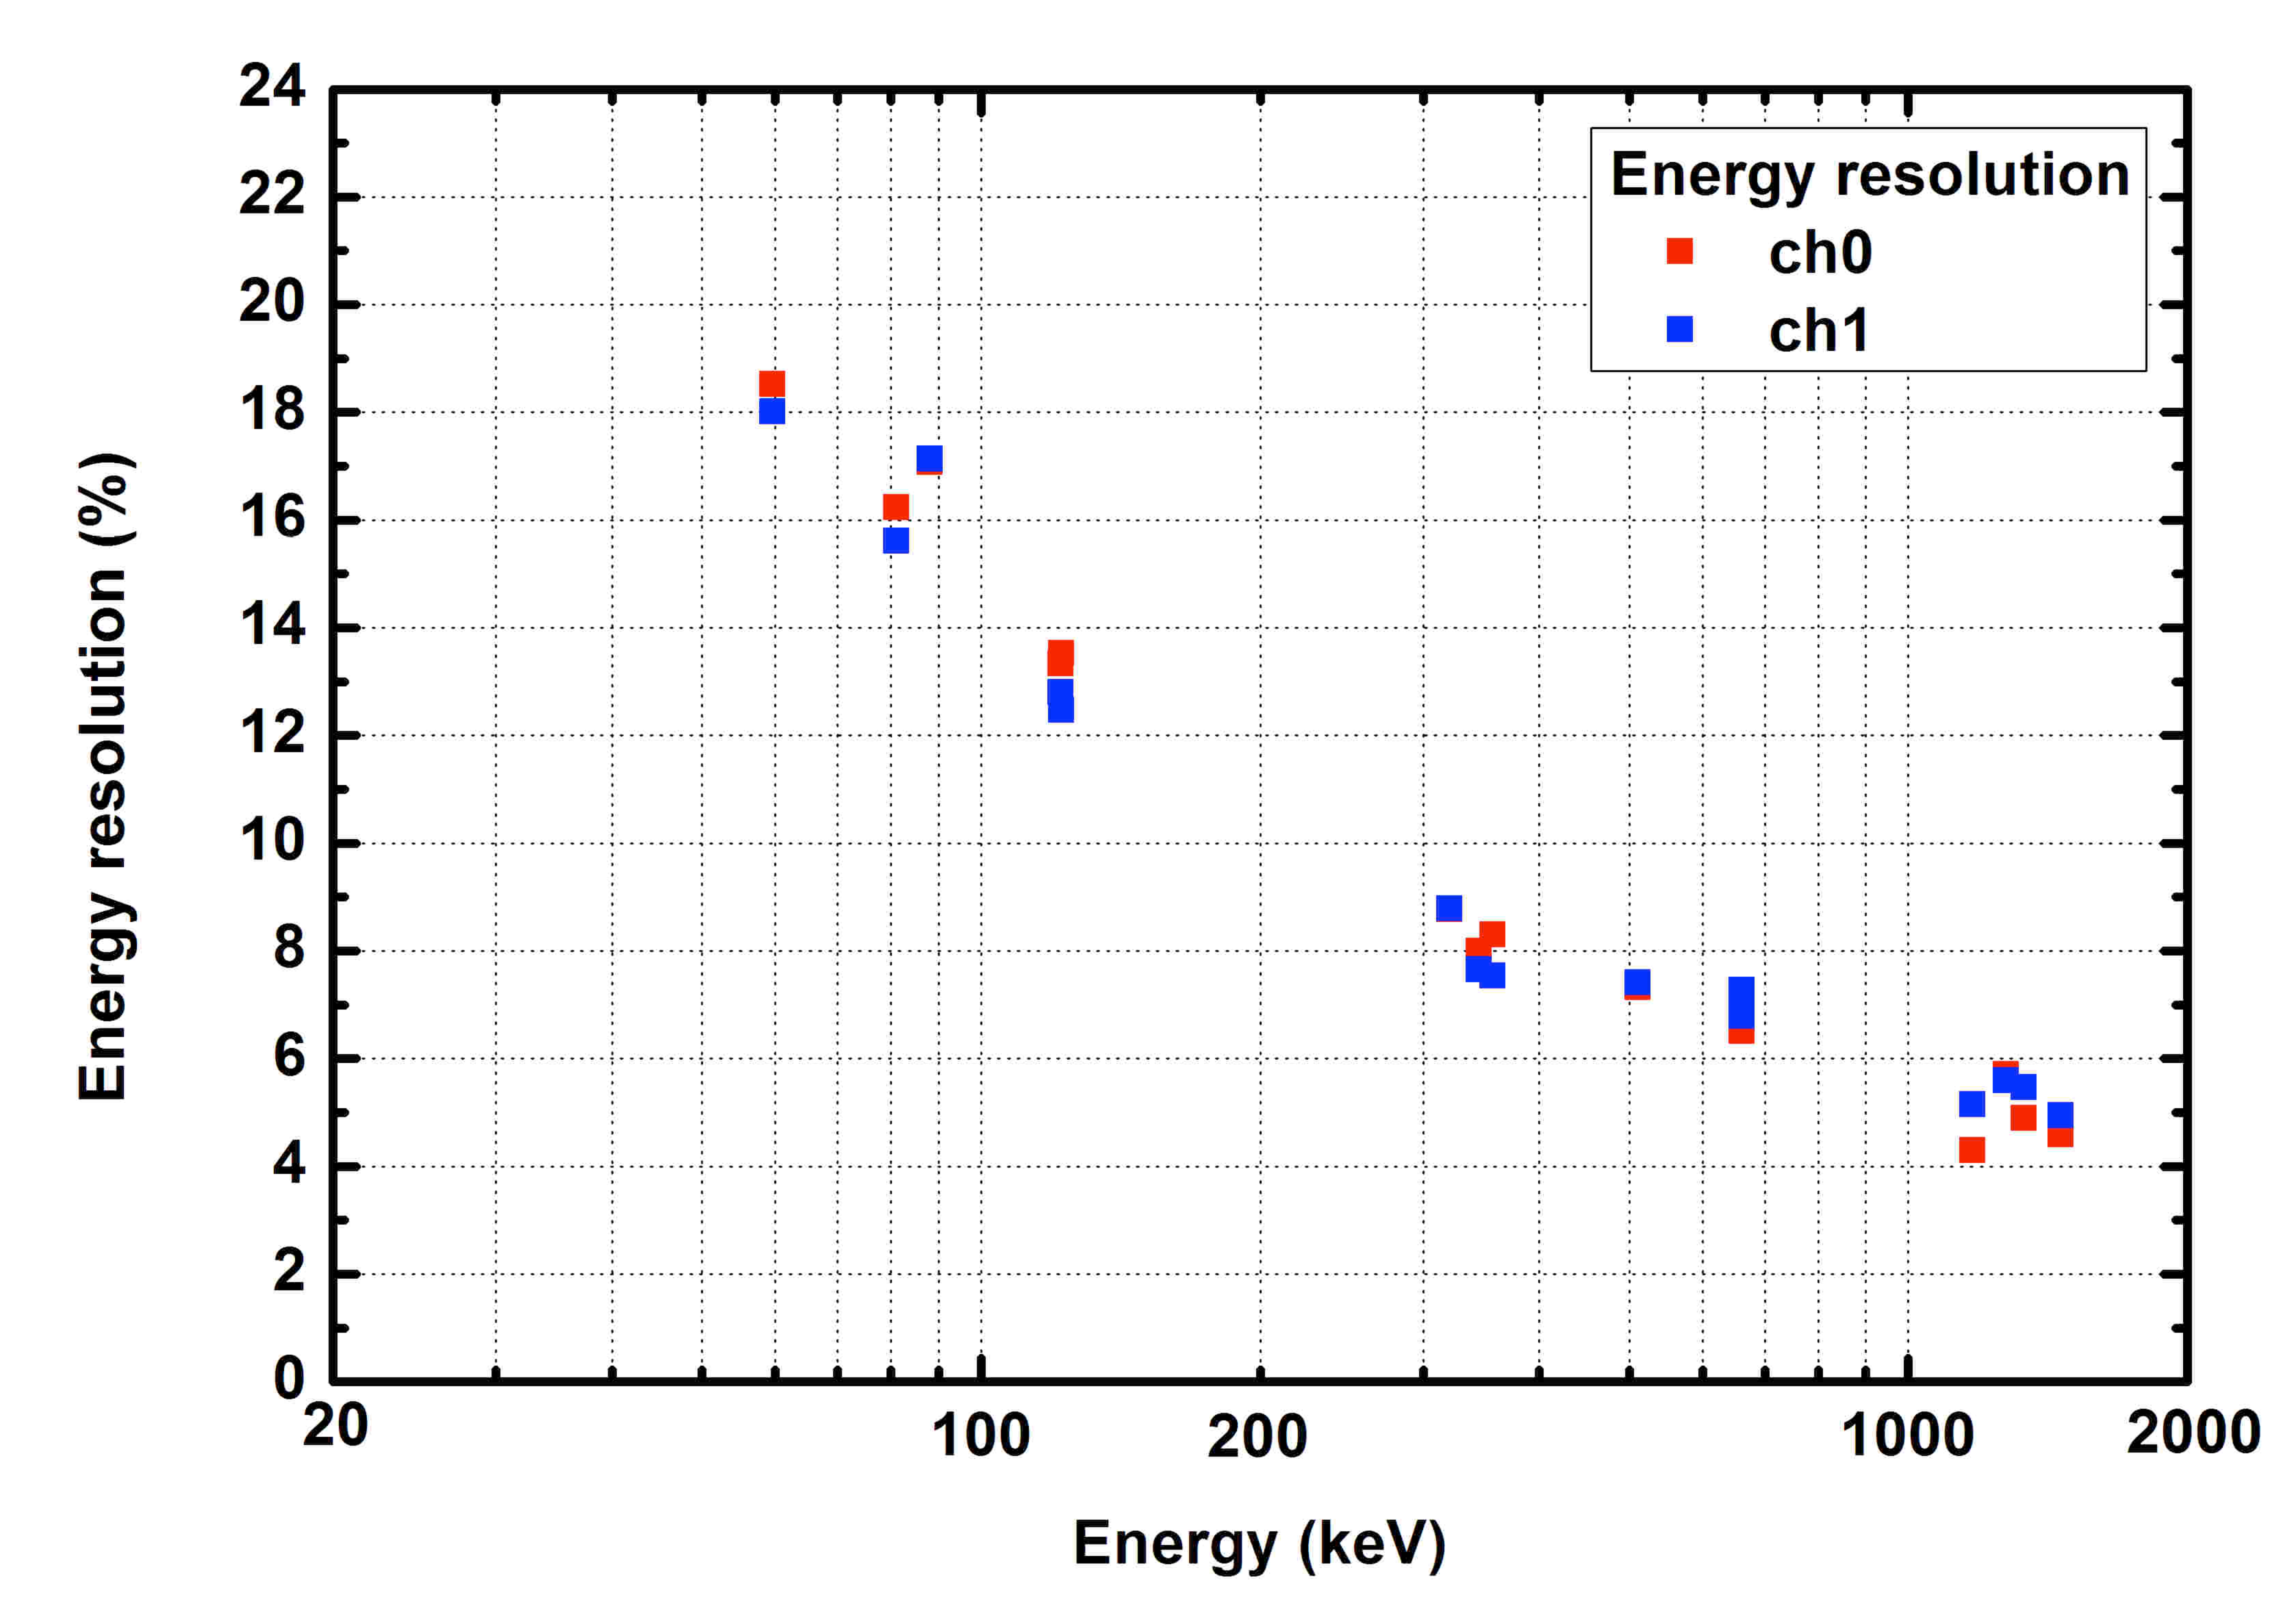
\includegraphics[width=74mm]{Chapter8/figures/energyResolutionXeGammaDetector.pdf}
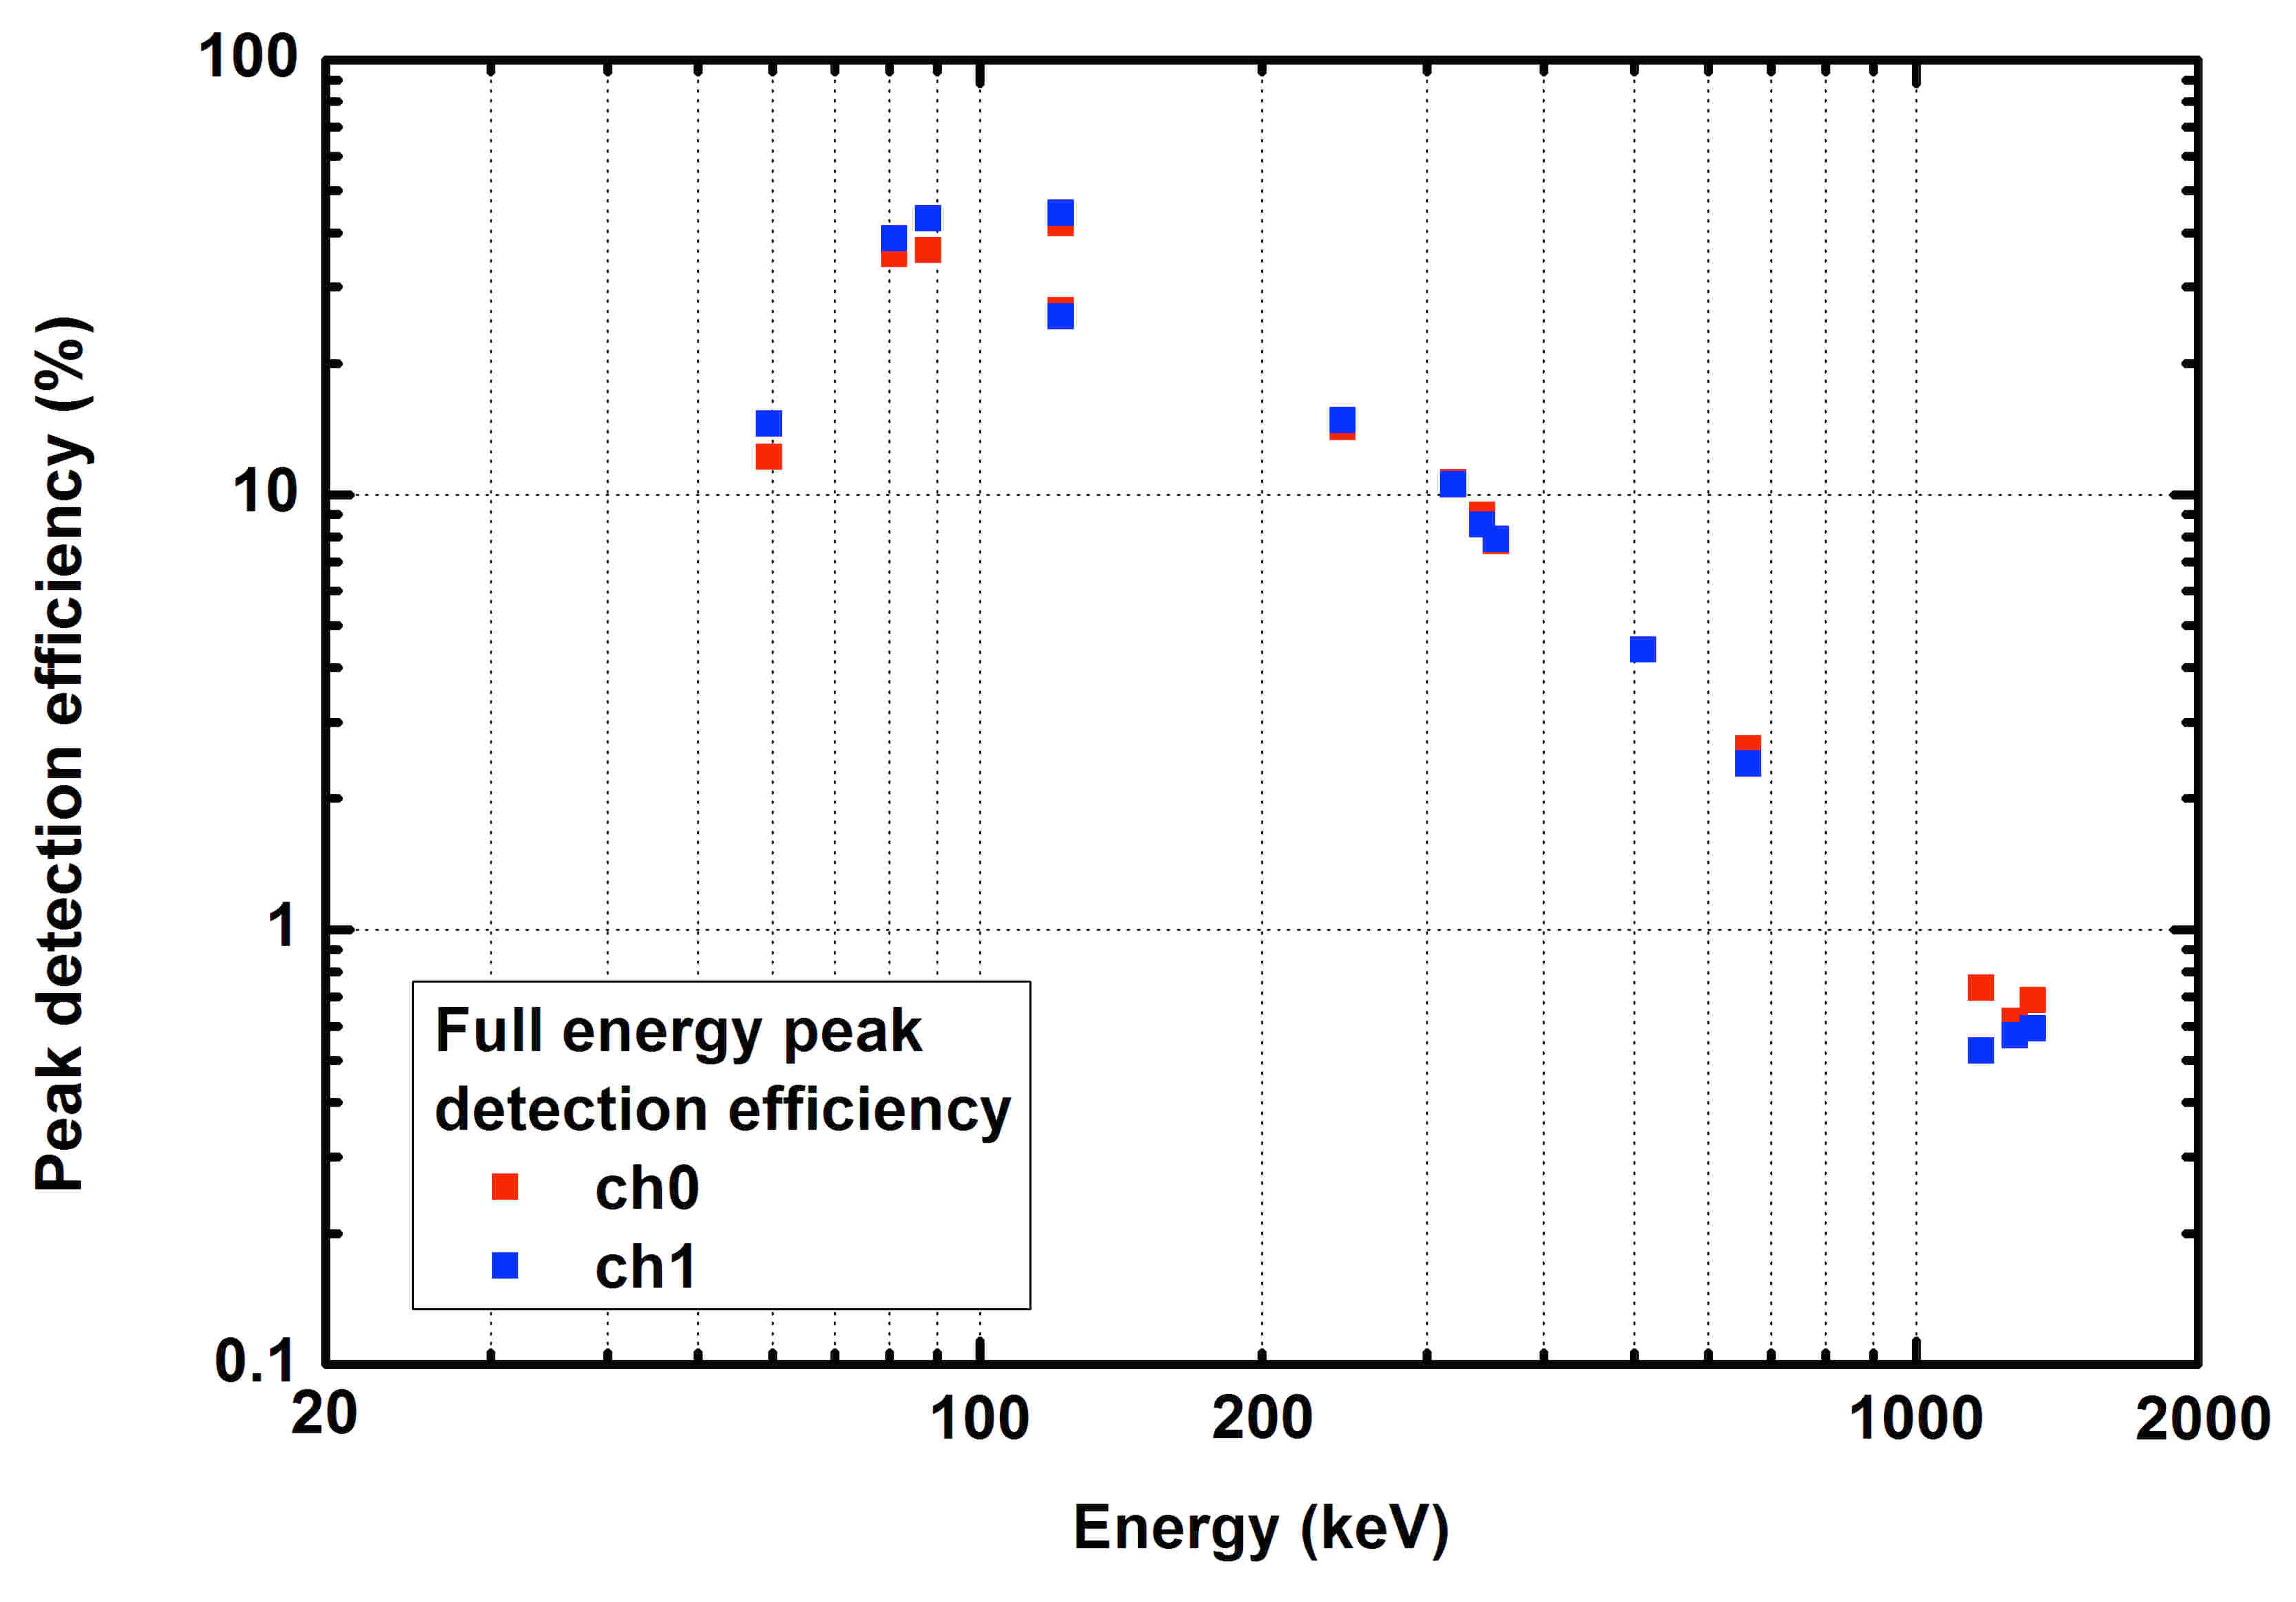
\includegraphics[width=74mm]{Chapter8/figures/efficienciesXeGammaDetector.pdf}
\caption{The xenon gamma detectors energy resolutions (left) and efficiencies (right) based on peak matching from 9 gamma sources with energies between 50 keV and 1.5 MeV. Plot taken from \cite{modesInternal}.}
\label{fig:modesXenonEnergyResolution}
\end{center}
\end{figure}

Although the xenon detector showed good energy resolutions at the higher energy range these studies showed very poor efficiencies also ($<$1\% above $>$1 MeV), with the detector failing to identify $^{22}$Na and $^{60}$Co sources. The right of figure \ref{fig:modesXenonEnergyResolution} shows the Peak Detection Efficiencies (PDEs) for the same 9 sources. The maximum efficiency is achieved at $\sim$100 keV reaching $\sim$50\% with it dropping off below this energy due to interactions in the Titanium vessel and decreasing above this energy due to decreased cross section.

\subsubsection{Detector Stability}
The $^{137}$Cs source was used to measure the stability and temperature response of the xenon detector. Measurements of the signal amplitude were taken at the 662 keV peak at 15 minute exposures, over a period 14 days to determine the detector stability. The left of figure \ref{fig:modesCs137Stability} shows the measured amplitudes for both channels, showing a fairly stable response (maximum $\sim$2.2\% deviation) over this period varying between 1130 - 1155 and 955 - 970 for the signal amplitude for channel 0 and 1 respectively.

The variation in the signal amplitude over this period cannot be solely attributed to the temperature variation as this was also measured independently by controlled cooling of the detector between 12$^{\circ}$C and 20$^{\circ}$C. The maximum deviation for this variation was at $\sim$0.9\%, this is negligible in comparison to the energy resolution at 662 keV of $\sim$7.0\%.

\begin{figure}[htbp]
\begin{center}
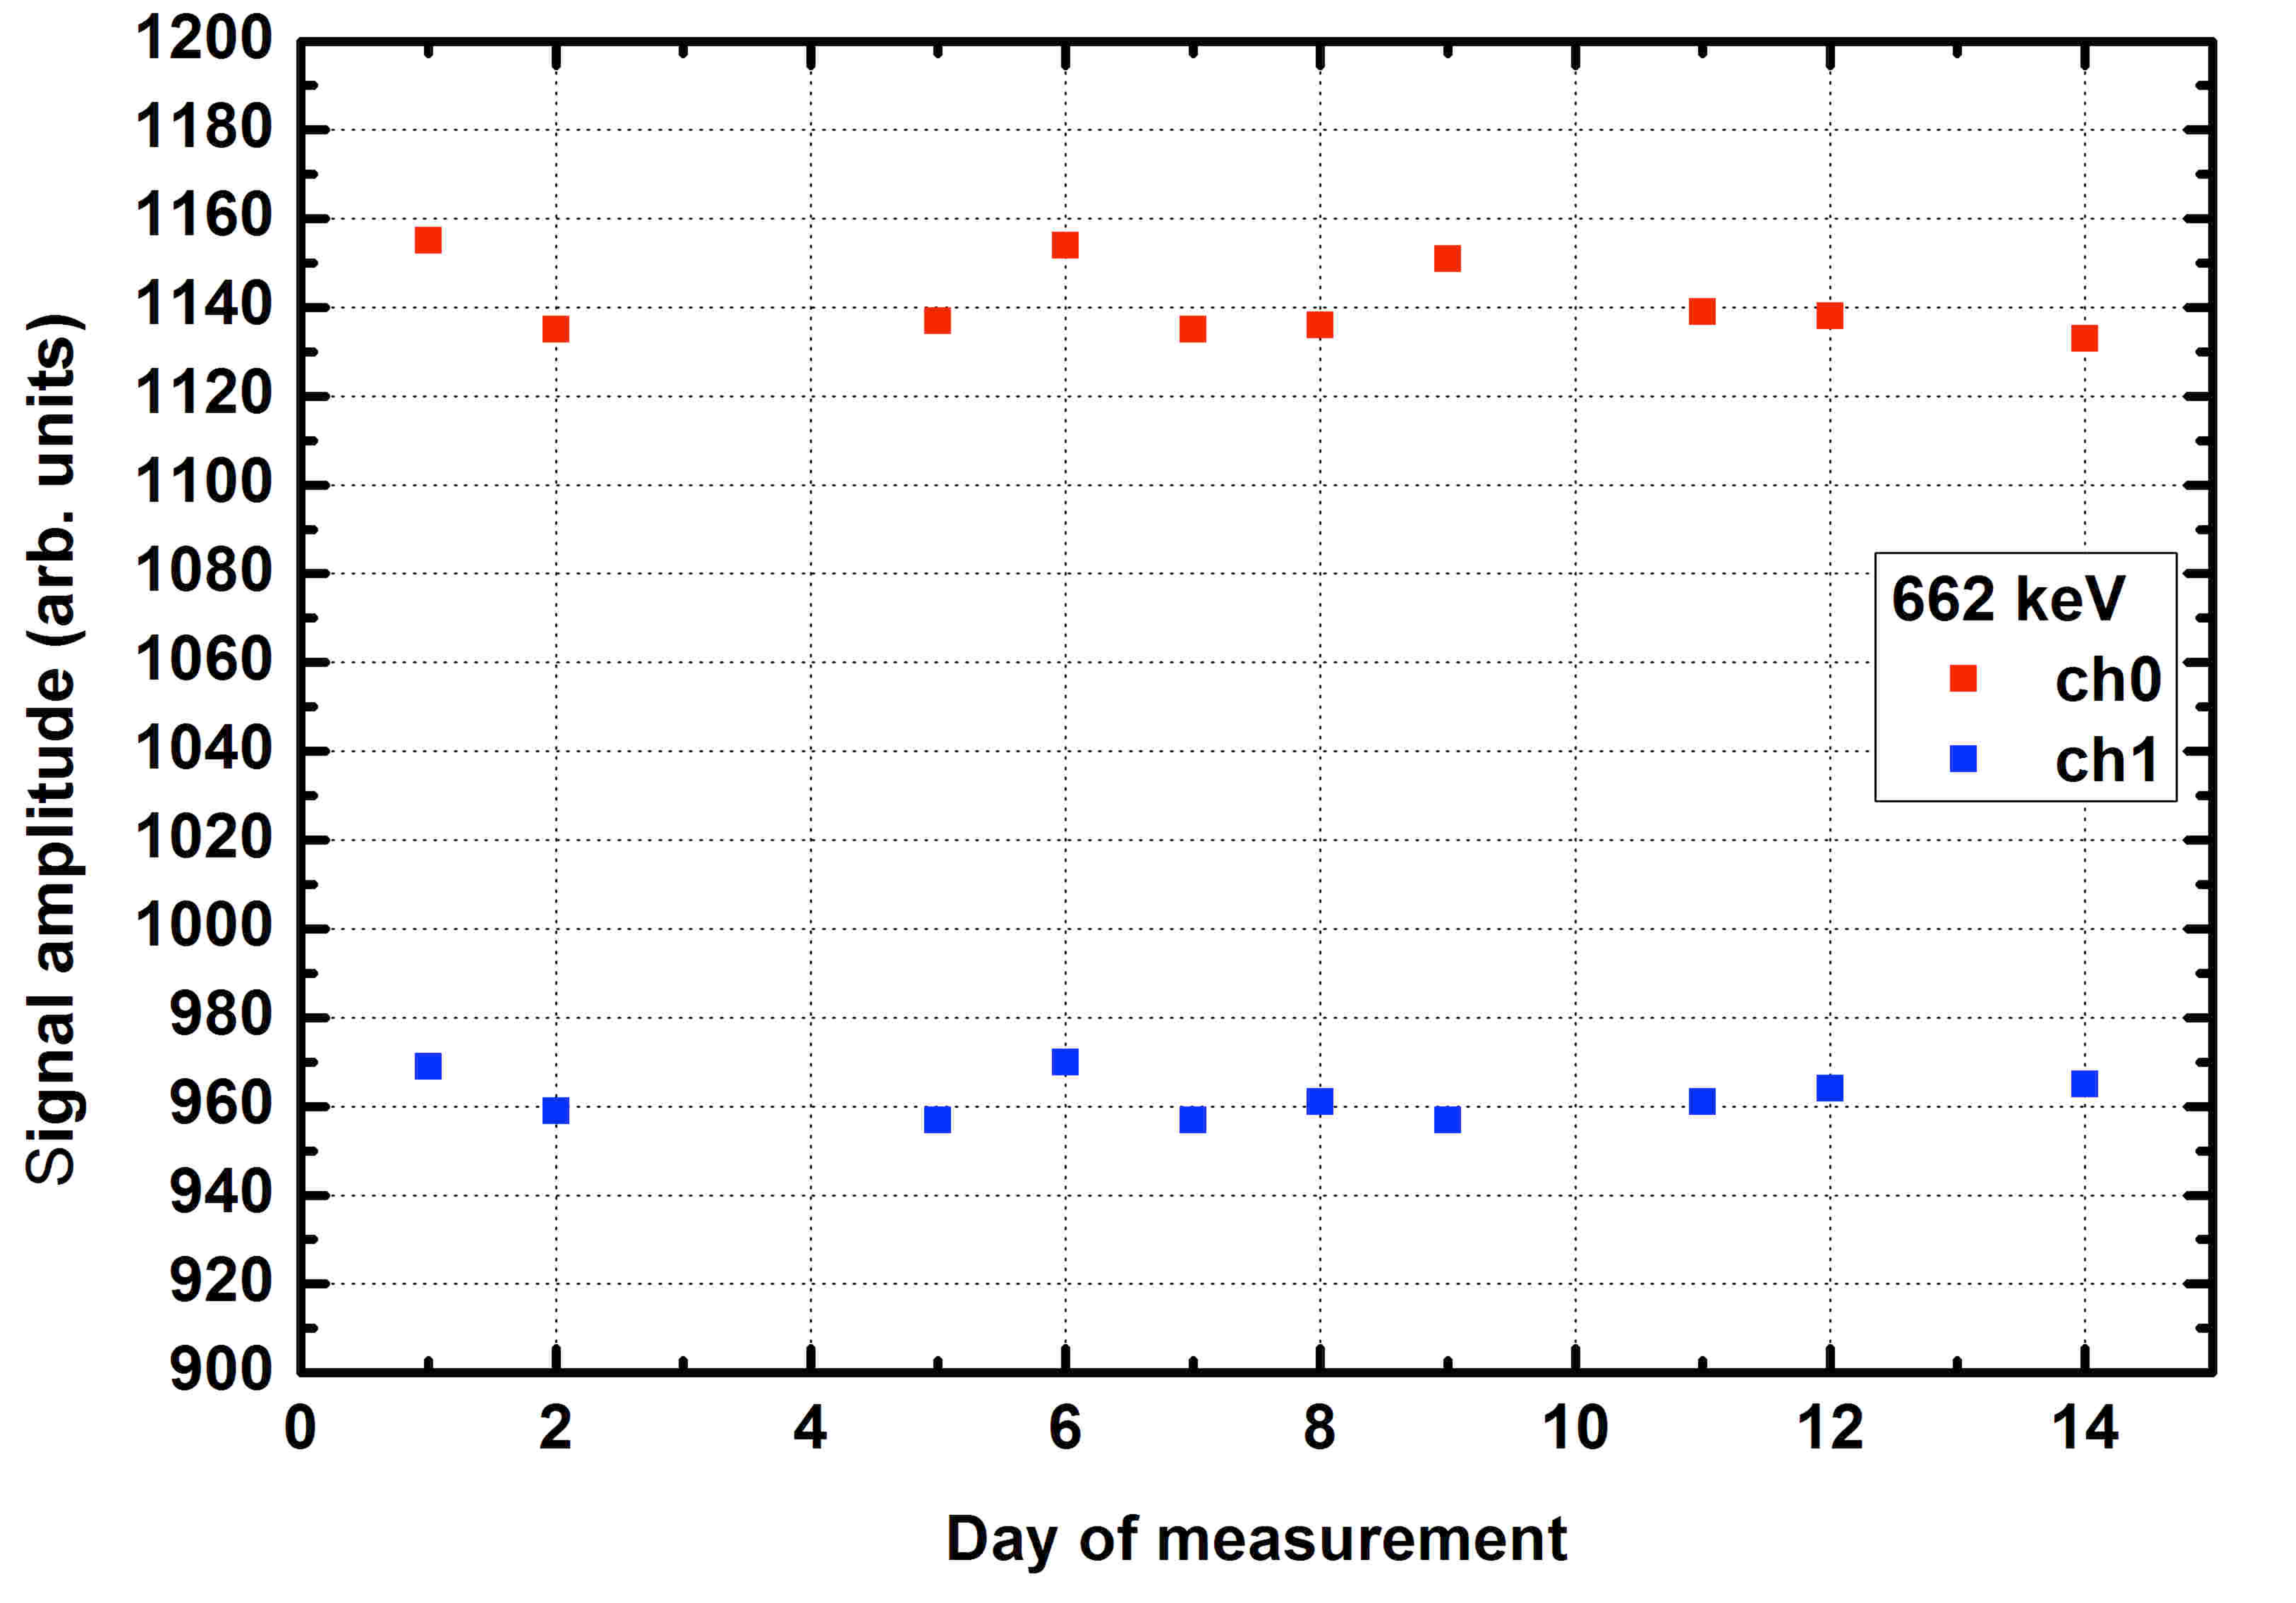
\includegraphics[width=76mm]{Chapter8/figures/Cs-137_XenonStability.pdf}
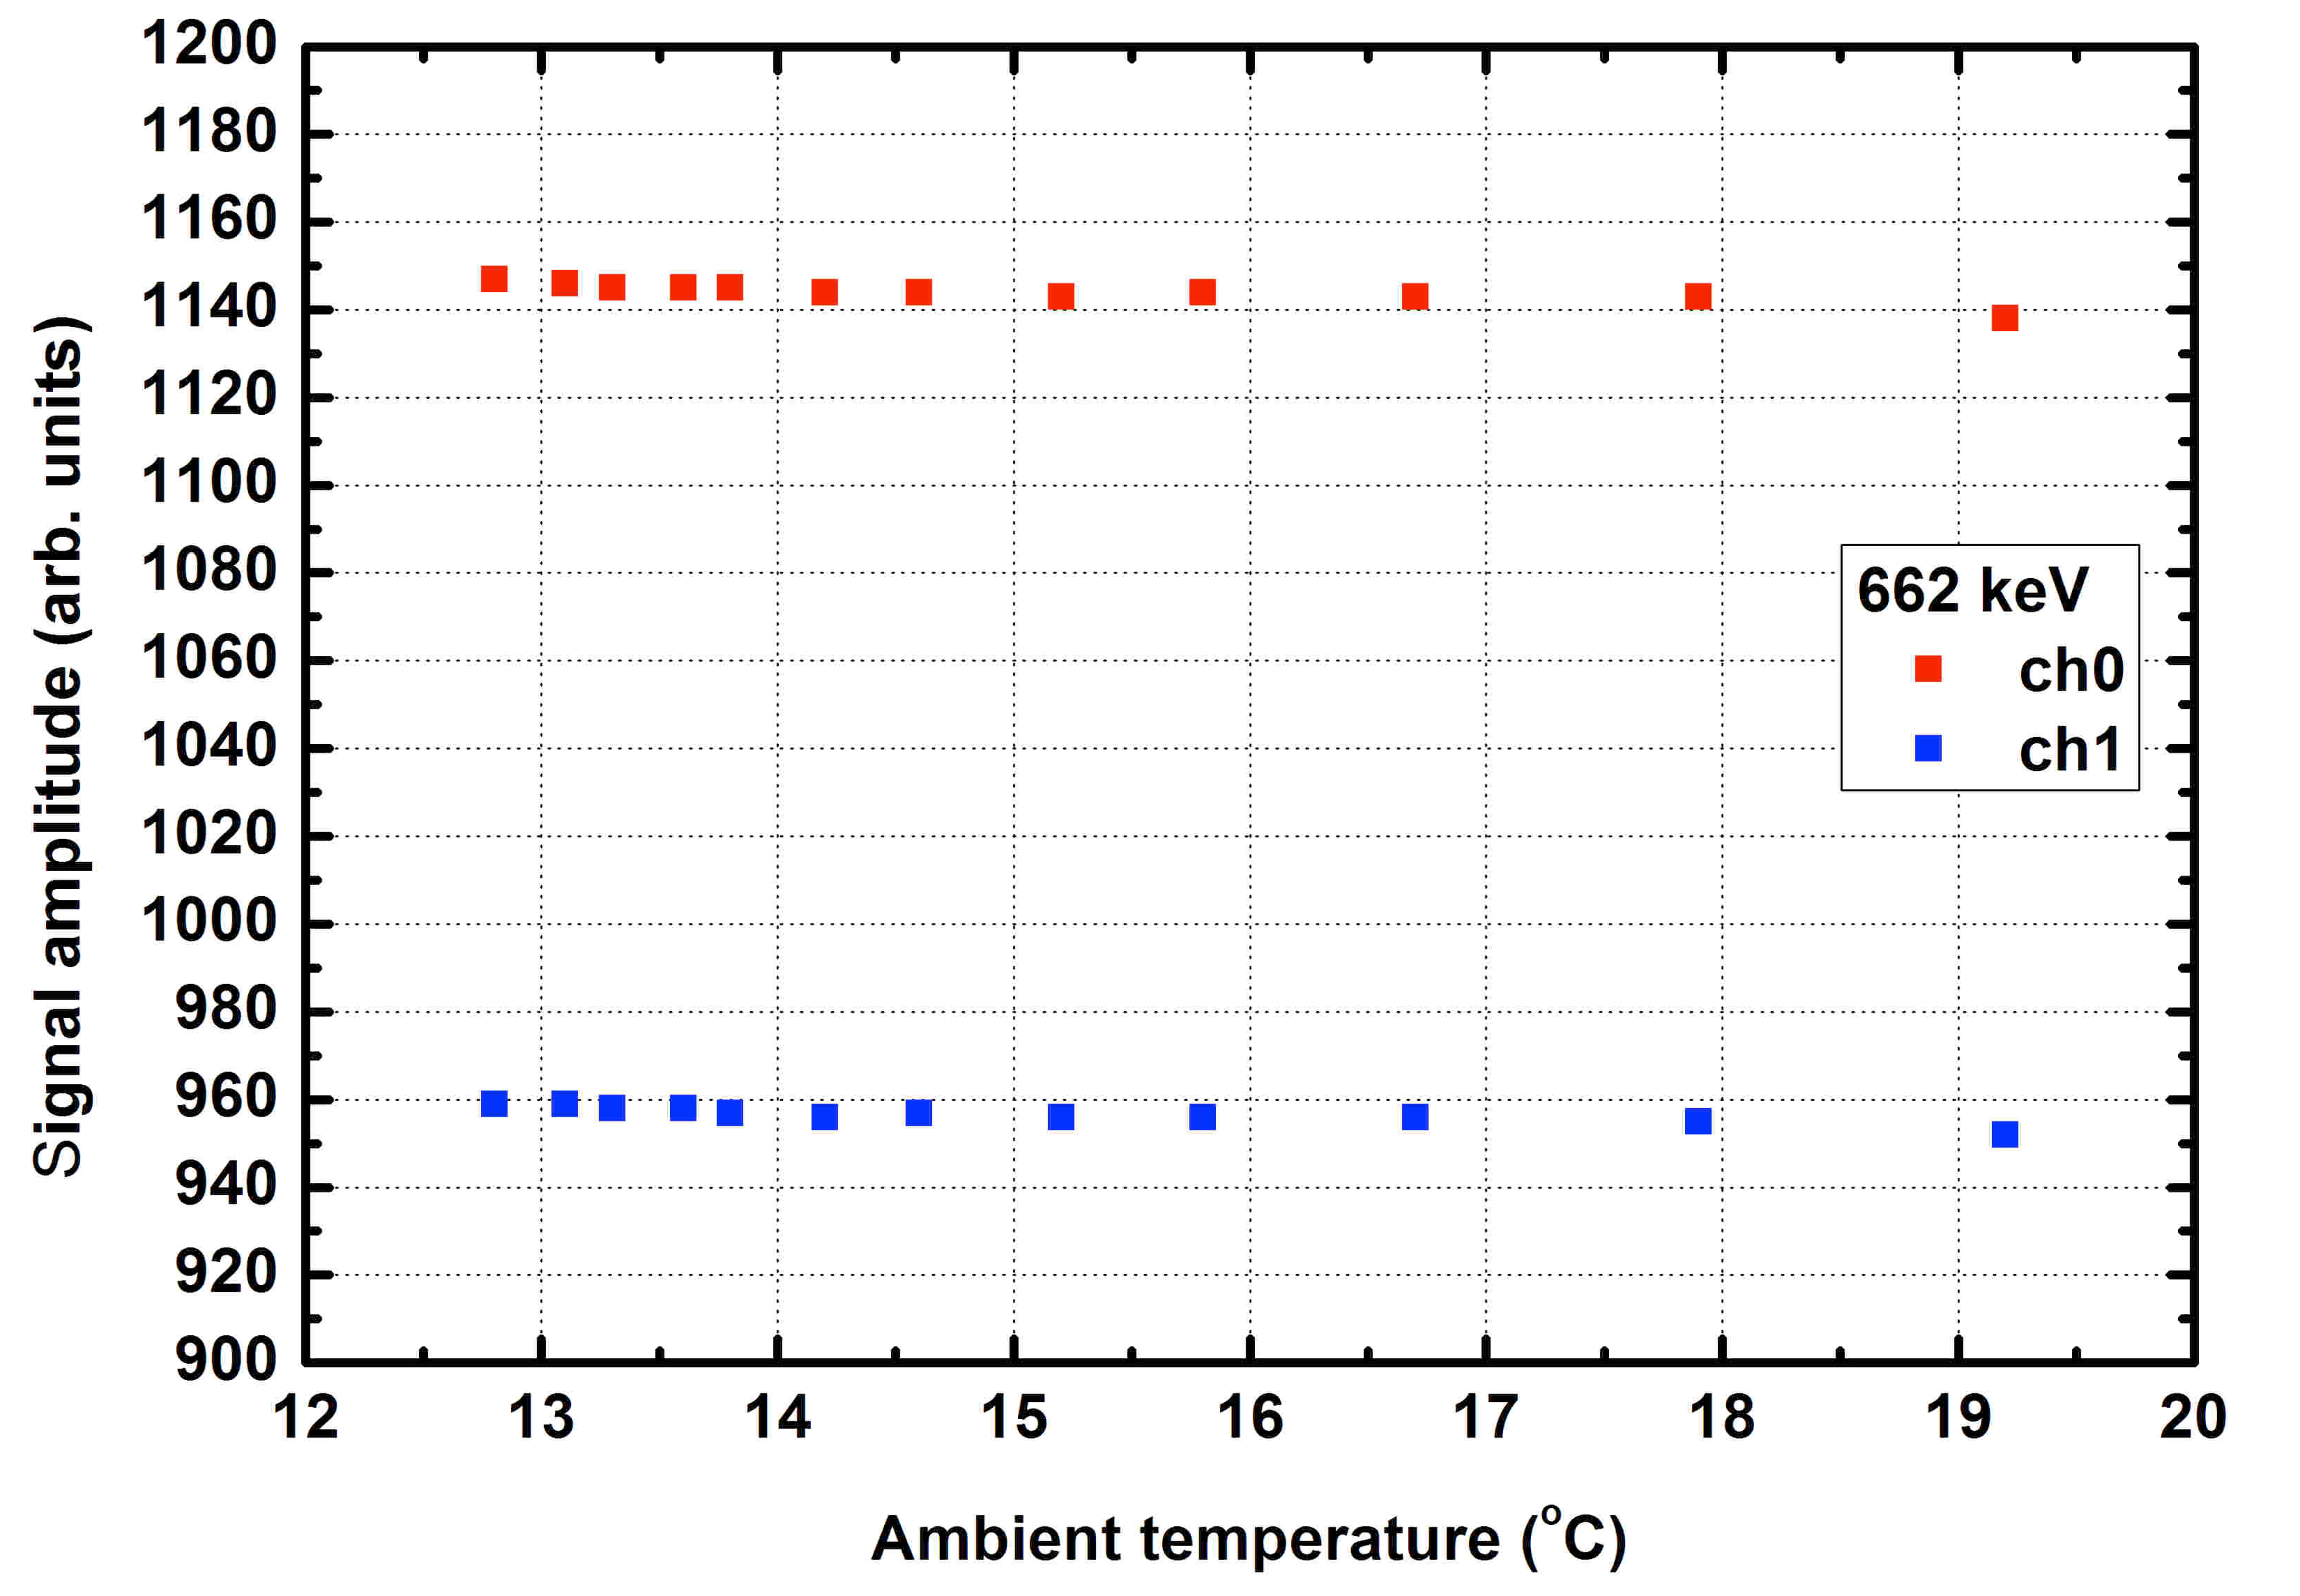
\includegraphics[width=76mm]{Chapter8/figures/Cs-137_XenonTempResponse.pdf}
\caption{The stability (left) and temperature dependance (right) and of the signal amplitude measured for a $^{137}$Cs source for both PMTs of the xenon detector. Plot taken from \cite{modesInternal}.}
\label{fig:modesCs137Stability}
\end{center}
\end{figure}

\subsubsection{Detection Rates}
To fulfil the prototype requirements controlled tests on the xenon detector were performed to determine the probability of detection and FAR for the three sources: $^{241}$Am, $^{137}$Cs and $^{60}$Co. The setup in figure \ref{fig:modesXenonSetup} shows the xenon detector placed at a variable distance away from the source fixed securely to a stand. The experiment was conducted in a large experimental hall to reduce the influence from wall interactions and the distance was varied to compensate for the variable strengths of the sources. The room temperature was measured between 20.3$^{\circ}$C and 21.6$^{\circ}$C with $\sim$35\% humidity and pressure $\sim$100 kPa. The gamma radiation background was measured at $\sim$0.11$\mu$Sv/h.

\begin{figure}[htbp]
\begin{center}
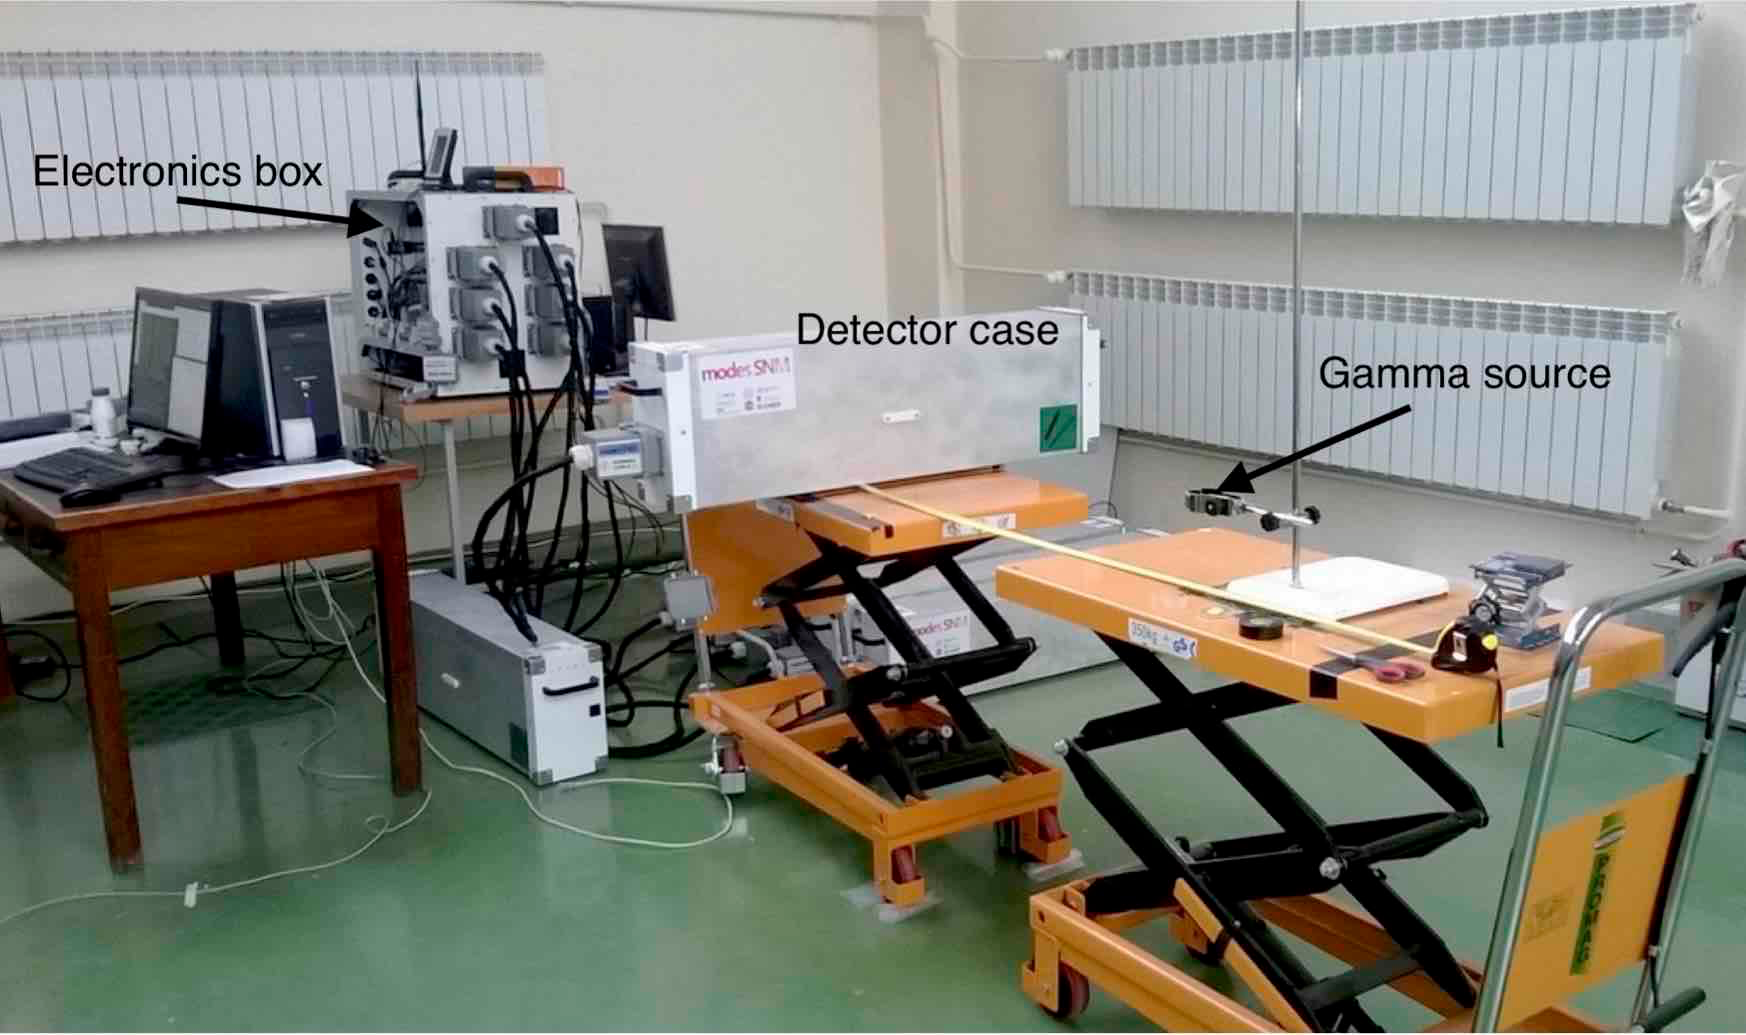
\includegraphics[width=120mm]{Chapter8/figures/XenonRatesTestSetup.pdf}
\caption{The experimental setup for detection rate tests on the xenon detector. The source is fixed to the clamp stand facing the detector box. Plot taken from \cite{modesInternal}.}
\label{fig:modesXenonSetup}
\end{center}
\end{figure}

A total of 450 consecutive tests were conducted for each of the three sources, each with an exposure time of 2 seconds. All the tests yielded a 100\% success rate, measuring a 97.6\% probability of detection at 95\% C.L \cite{modesInternal}. The FAR did not exceed 1 per hour.

For source identification 9 sources were used: $^{137}$Cs (662 keV), $^{60}$Co (1.17 \& 1.33 MeV),$^{22}$Na (511 keV \& 1.28 MeV), $^{152}$Eu (122, 245, 344, 779 keV \& 1.41 MeV), $^{51}$Cr (320 keV), $^{133}$Ba (81, 276/303 \& 356/384 keV), $^{57}$Co (122 keV), $^{241}$Am (59.6 keV) and $^{109}$Cd (22 \& 88 keV). The exposure times were increased to 60 second per identification and sources were adjusted by distance to provide 50 nSv/h dose rates at the detector. The experimental environment and apparatus was otherwise not altered. For sources with peak energies below 1 MeV, 60 s was an adequate exposure time with the system able to identify the source correctly in this time frame. However for energies above this threshold the detector efficiencies were too low to provide a successful identification for $^{60}$Co, with nether peak shown in the spectra, shown in figure \ref{fig:modesXenonSourceTests}.

\begin{figure}[htbp]
\begin{center}
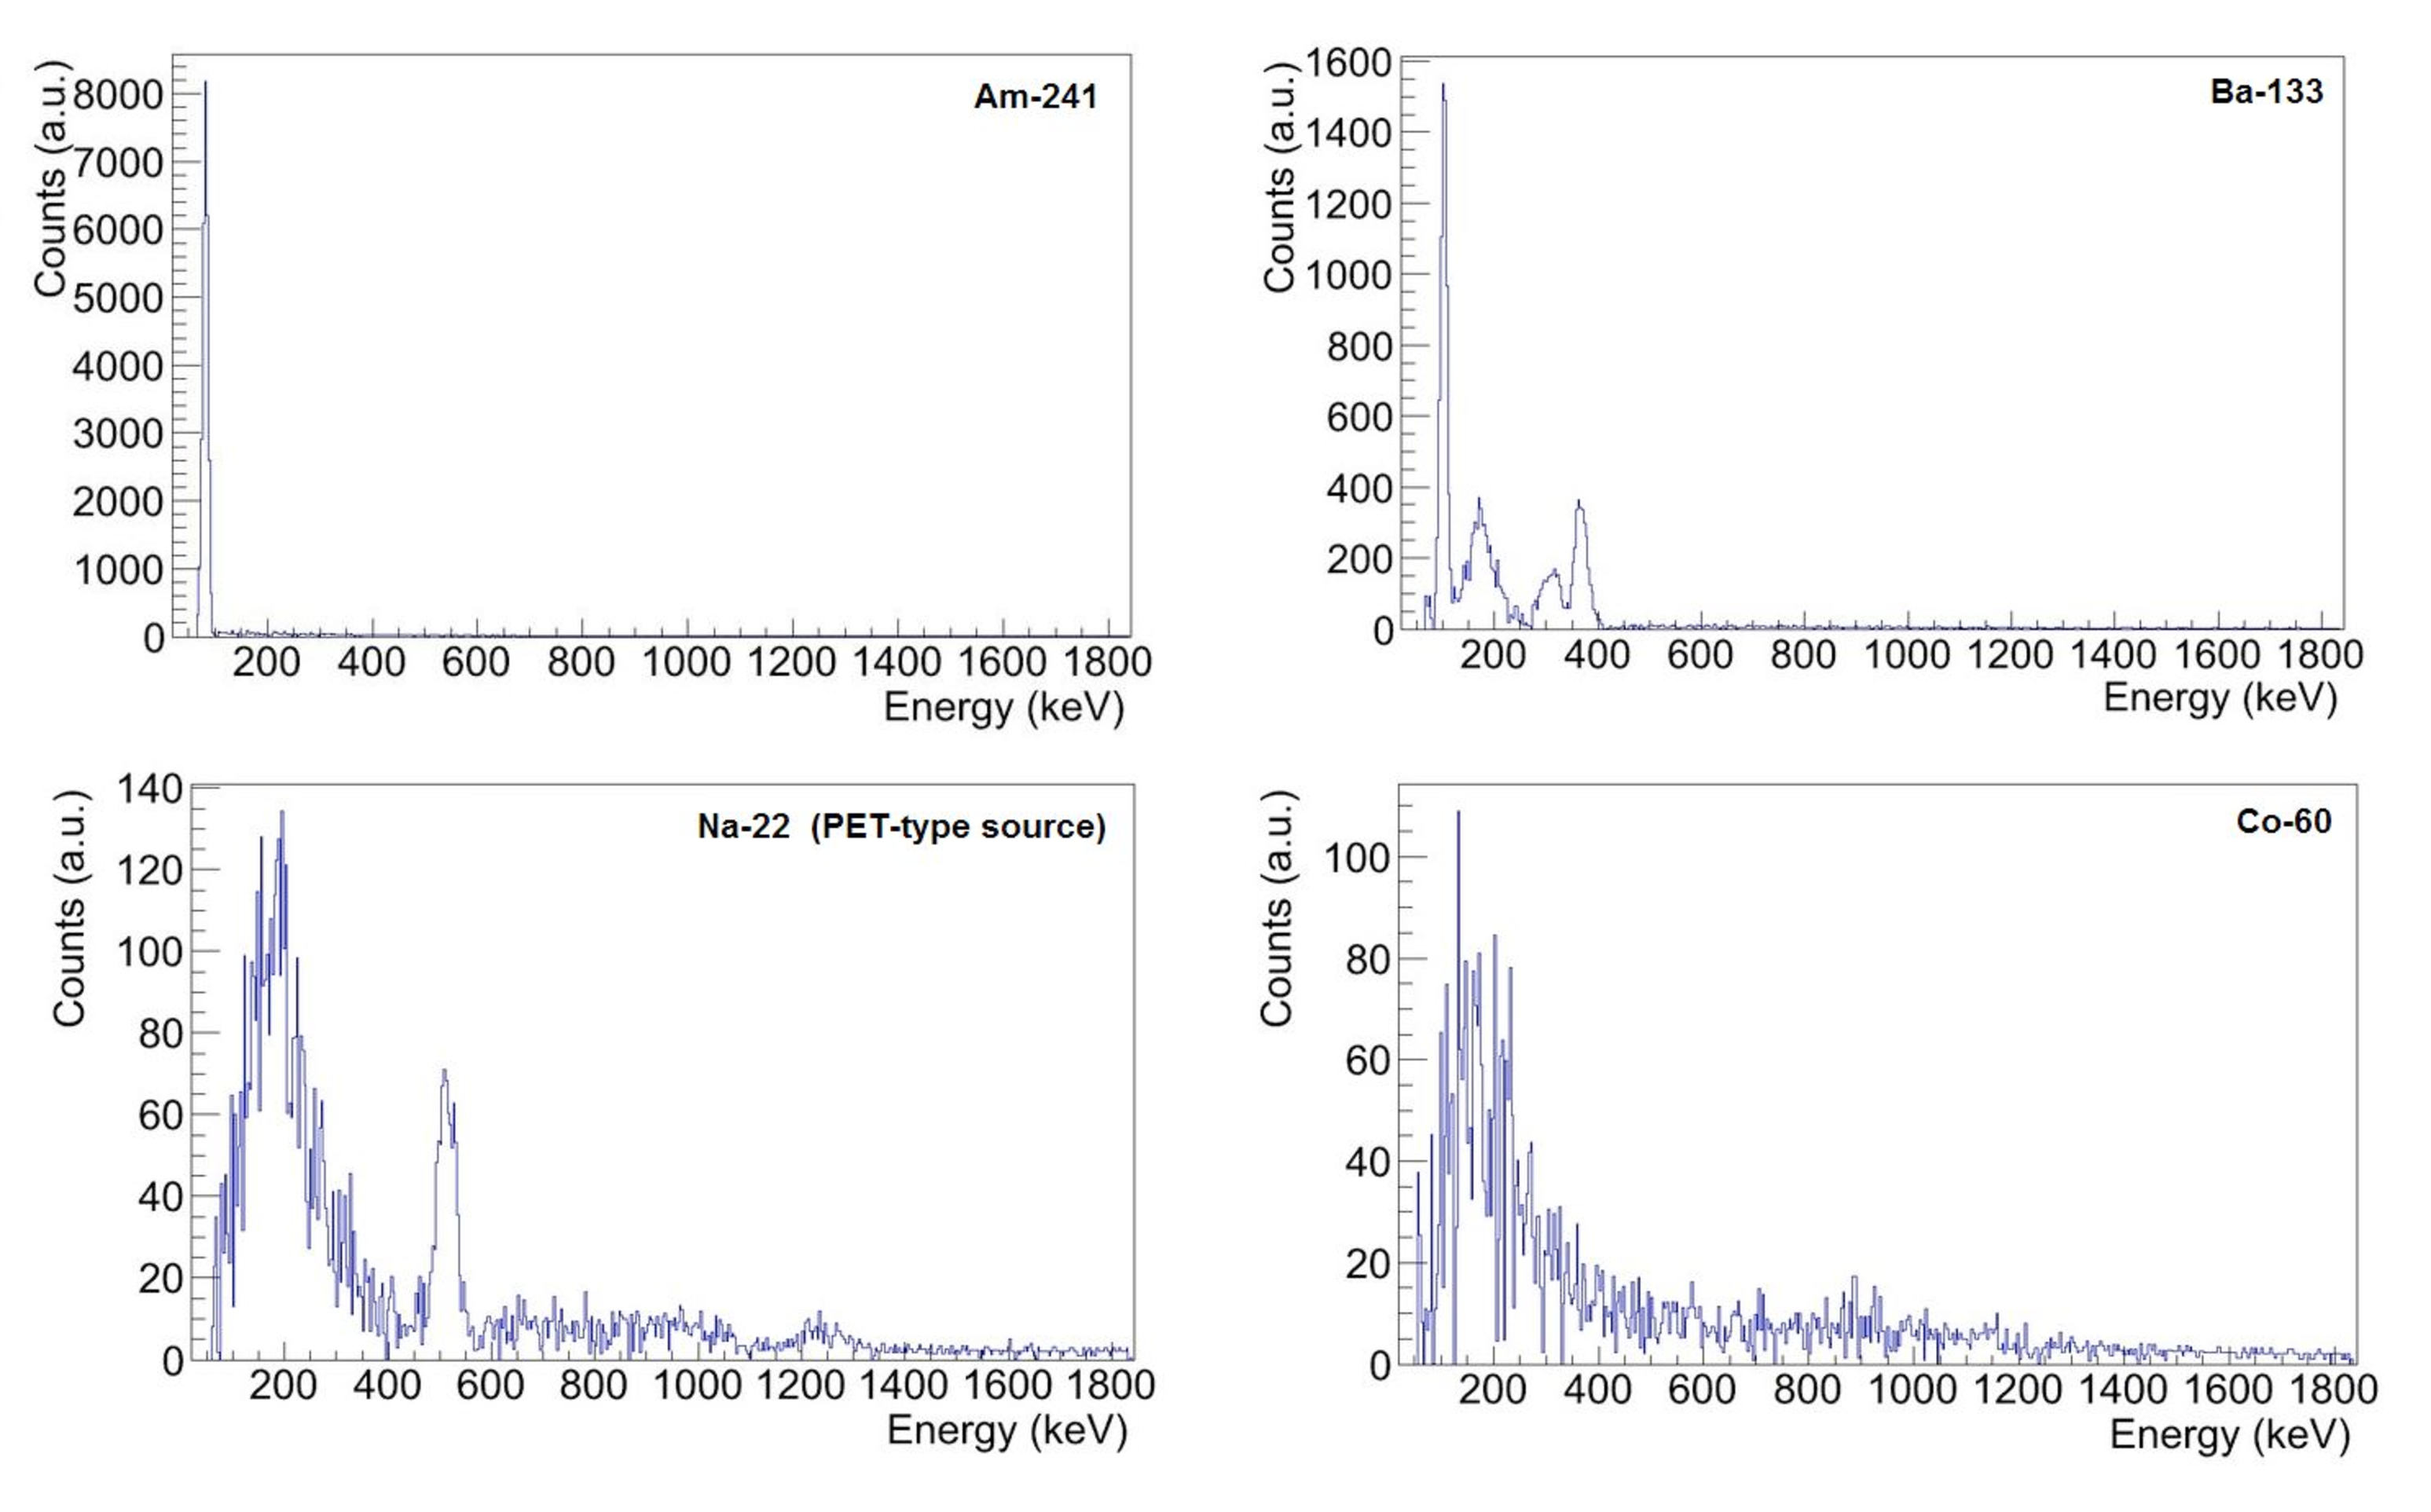
\includegraphics[width=110mm]{Chapter8/figures/XenonSourceIdentification.pdf}
\caption{The energy spectra measured with the channel 0 of the xenon detector for sources: $^{241}$Am (upper left), $^{133}$Ba (upper right), $^{22}$Na (lower left) and $^{60}$Co (lower right). The peaks can be noticed for all sources except the 1.28 MeV on $^{22}$Na and both for $^{60}$Co. Plot taken from \cite{modesInternal}.}
\label{fig:modesXenonSourceTests}
\end{center}
\end{figure}

\subsection{Fast Neutron Detector Response}
Good gamma rejection is an important property for the neutron detectors as this can be a cause for an increased false alarm rate. The neutron gamma discrimination is performed by use of the PSD value, equation \ref{eq:modesPsdValue}, by comparing the difference between the long and short gate integrations with the pulse height, which is proportional to the long gate integration. Figure \ref{fig:neutronPsdCut} shows the PSD value binned as a function of pulse height for a fast neutron detector exposed to a neutron/gamma source. Two clear groups of events can be noticed, showing neutrons occupying the higher PSD region at a fairly constant value of 0.8, compared to the gammas with a more variable lower PSD value. The difference can be attributed to neutrons causing recoil of the $^{4}$He nucleus and therefore very localised energy deposition compared to the electron recoil for gamma interactions which deposits less energy (tens of keV/cm). Studies have shown \cite{helium4Detectors} that while the short gate integration (fast component) for both interactions is $\sim$120 mV for a typical event in $^{4}$He, the slow scintillation component is $\sim$3-4 times larger for neutrons.

\begin{figure}[htbp]
\begin{center}
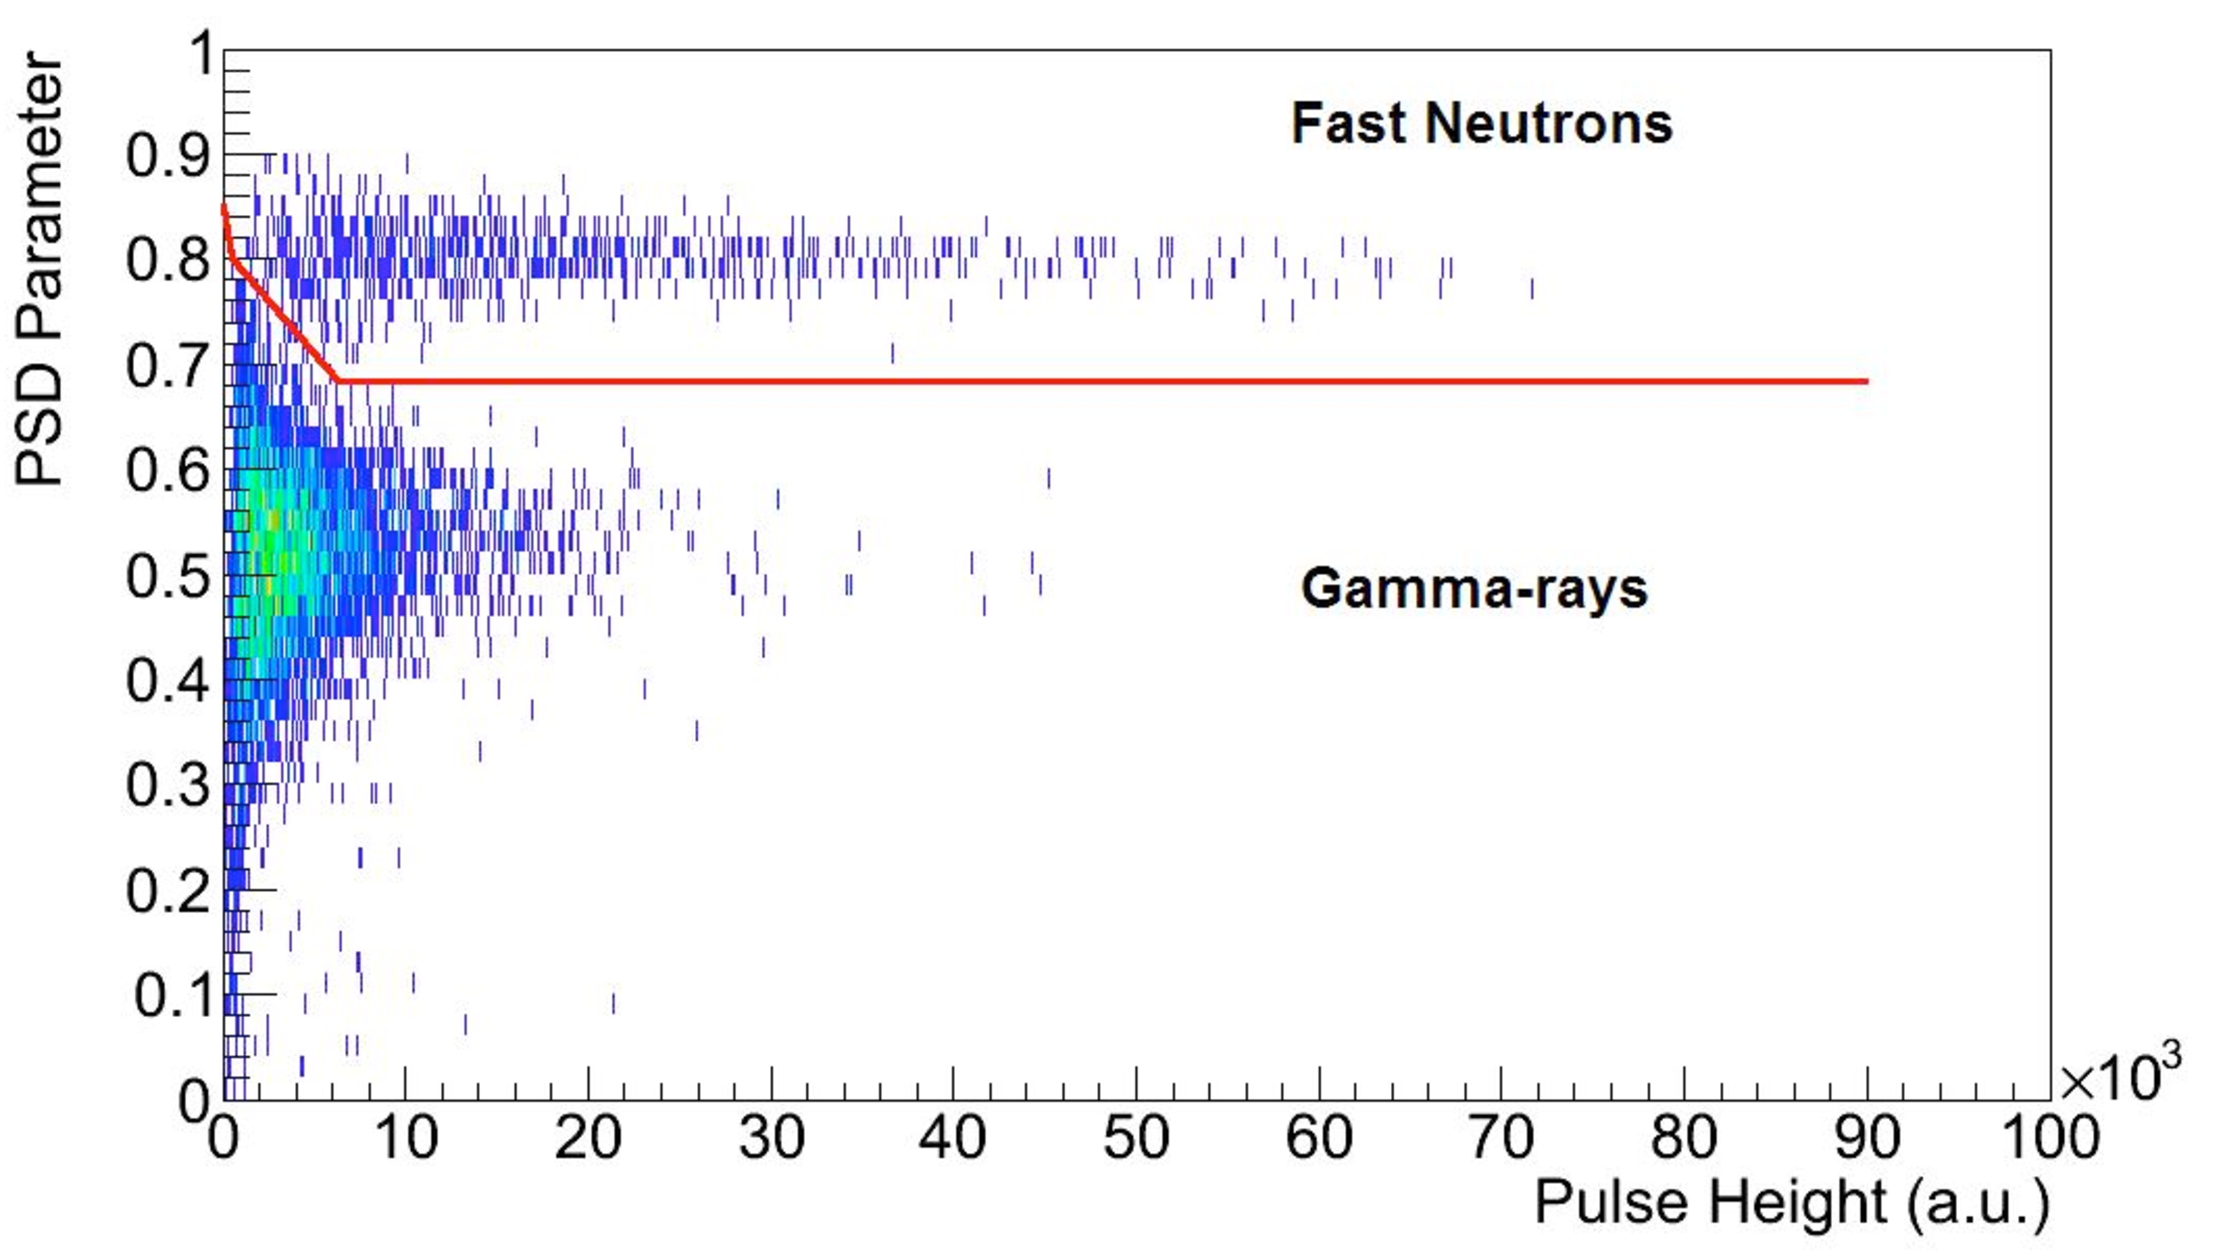
\includegraphics[width=90mm]{Chapter8/figures/psdCut.pdf}
\caption{The PSD value binned as a function of the pulse height (proportional to the total integrated charge) an event by event basis from events in the fast neutron detector from a neutron/gamma source. Both channels on the neutron detector are used. Plot taken from \cite{modesInternal}.}
\label{fig:neutronPsdCut}
\end{center}
\end{figure}

\subsubsection{Detection Rates}
To measure the probability of detection for the fast neutron detectors, each detector case (2 in each) was exposed to a $^{252}$Cf source following the same method and setup as the xenon detector. The $^{252}$Cf source of 570 kBq activity was placed at 2.28 m from the detector case to provide a 0.1 ns$^{-1}$cm$^{-2}$ at the detectors. Again 2 second exposures were used to keep the FAR below 1 per hour and 449 trials were conducted \cite{modesInternal}. By summing the neutron events from each of the eight detectors the probability of detection reached 97.4\% at 95\% C.L, with 448/449 trials successful. It can be noted that with only half the detectors included a probability of detection of almost the required level (90\% at 95\% C.L) was reached with a probability of detection of 89.4\% at 95\% C.L \cite{modesInternal}

\subsection{Thermal Neutron Detector Response}
Determination of thermal neutrons is performed by comparison of the fast and slow components of the scintillation light. These values are equivalent to the Q$_{short}$ and Q$_{long}$ - Q$_{short}$ values respectively, which are determined from the integration gates. Figure \ref{fig:thermalFastNeutronCut} shows the 2-dimensional scatter plot binned by short and long scintillation components for events in the thermal neutron detector. The cuts shown are used within the MODES-SNM software to discriminate between fast neutrons, thermal neutrons and gammas within the thermal neutron detector. Optimisation studies within the collaboration have been performed to set these thresholds via exposure to intense neutron and gamma sources \cite{modesInternal}. The separation between fast and thermal neutrons is set at 1100 a.u on the fast component and the separation between thermals and gammas is set 600 a.u on the slow component. 

\begin{figure}[htbp]
\begin{center}
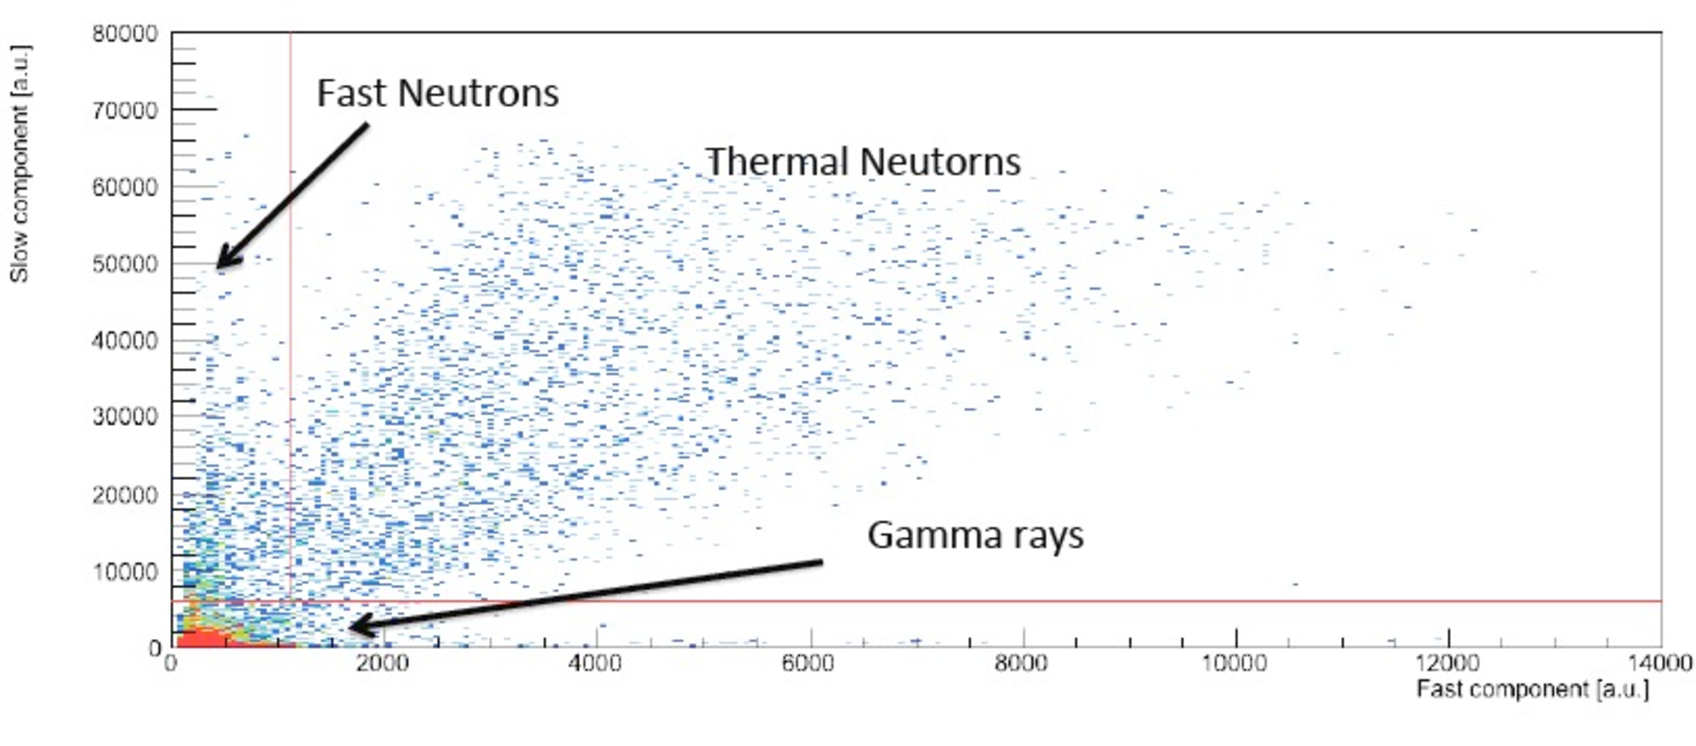
\includegraphics[width=140mm]{Chapter8/figures/thermalToFastNeutronCut.pdf}
\caption{A 2-dimensional plot for events in the thermal neutron detector binned according to each fast and slow component (Q$_{short}$ and Q$_{long}$ - Q$_{short}$ respectively) of the scintillation light. Two thresholds are set, shown as red lines, in order to discriminate between fast and thermal neutrons (1100 a.u on the fast component) and between gammas and thermal neutrons (600 a.u on the slow component). Plot taken from \cite{modesInternal}.}
\label{fig:thermalFastNeutronCut}
\end{center}
\end{figure}

Thermal neutrons are used within the MODES-SNM system to detect the presence of a  hydrogen rich shield around the source. Fast neutrons will interact with polyethylene such that it is possible for 100\% kinetic energy transfer per scatter, this can thermalise neutrons and increase their detection rate while reducing the fast neutron rate. A significant difference in fast/thermal neutron ratios can suggest a shielded source. 

For the purpose of an experiment, polyethylene was used as a shield to surround the $^{252}$Cf source. Blocks of the material were used to completely cover the source such that each face had 10 cm thick of polyethylene, except for the side facing the detector with only 5 cm thick polyethylene, as seen in figure \ref{fig:thermalNeutronCf252Shielded}. 

Measurements of the fast and thermal neutron rates were made in 60 second exposures for with and without the shielding present. The distance between the front of the detector case and the centre of the source was kept at 40 cm for both the shielded and unshielded source. 

\begin{figure}[htbp]
\begin{center}
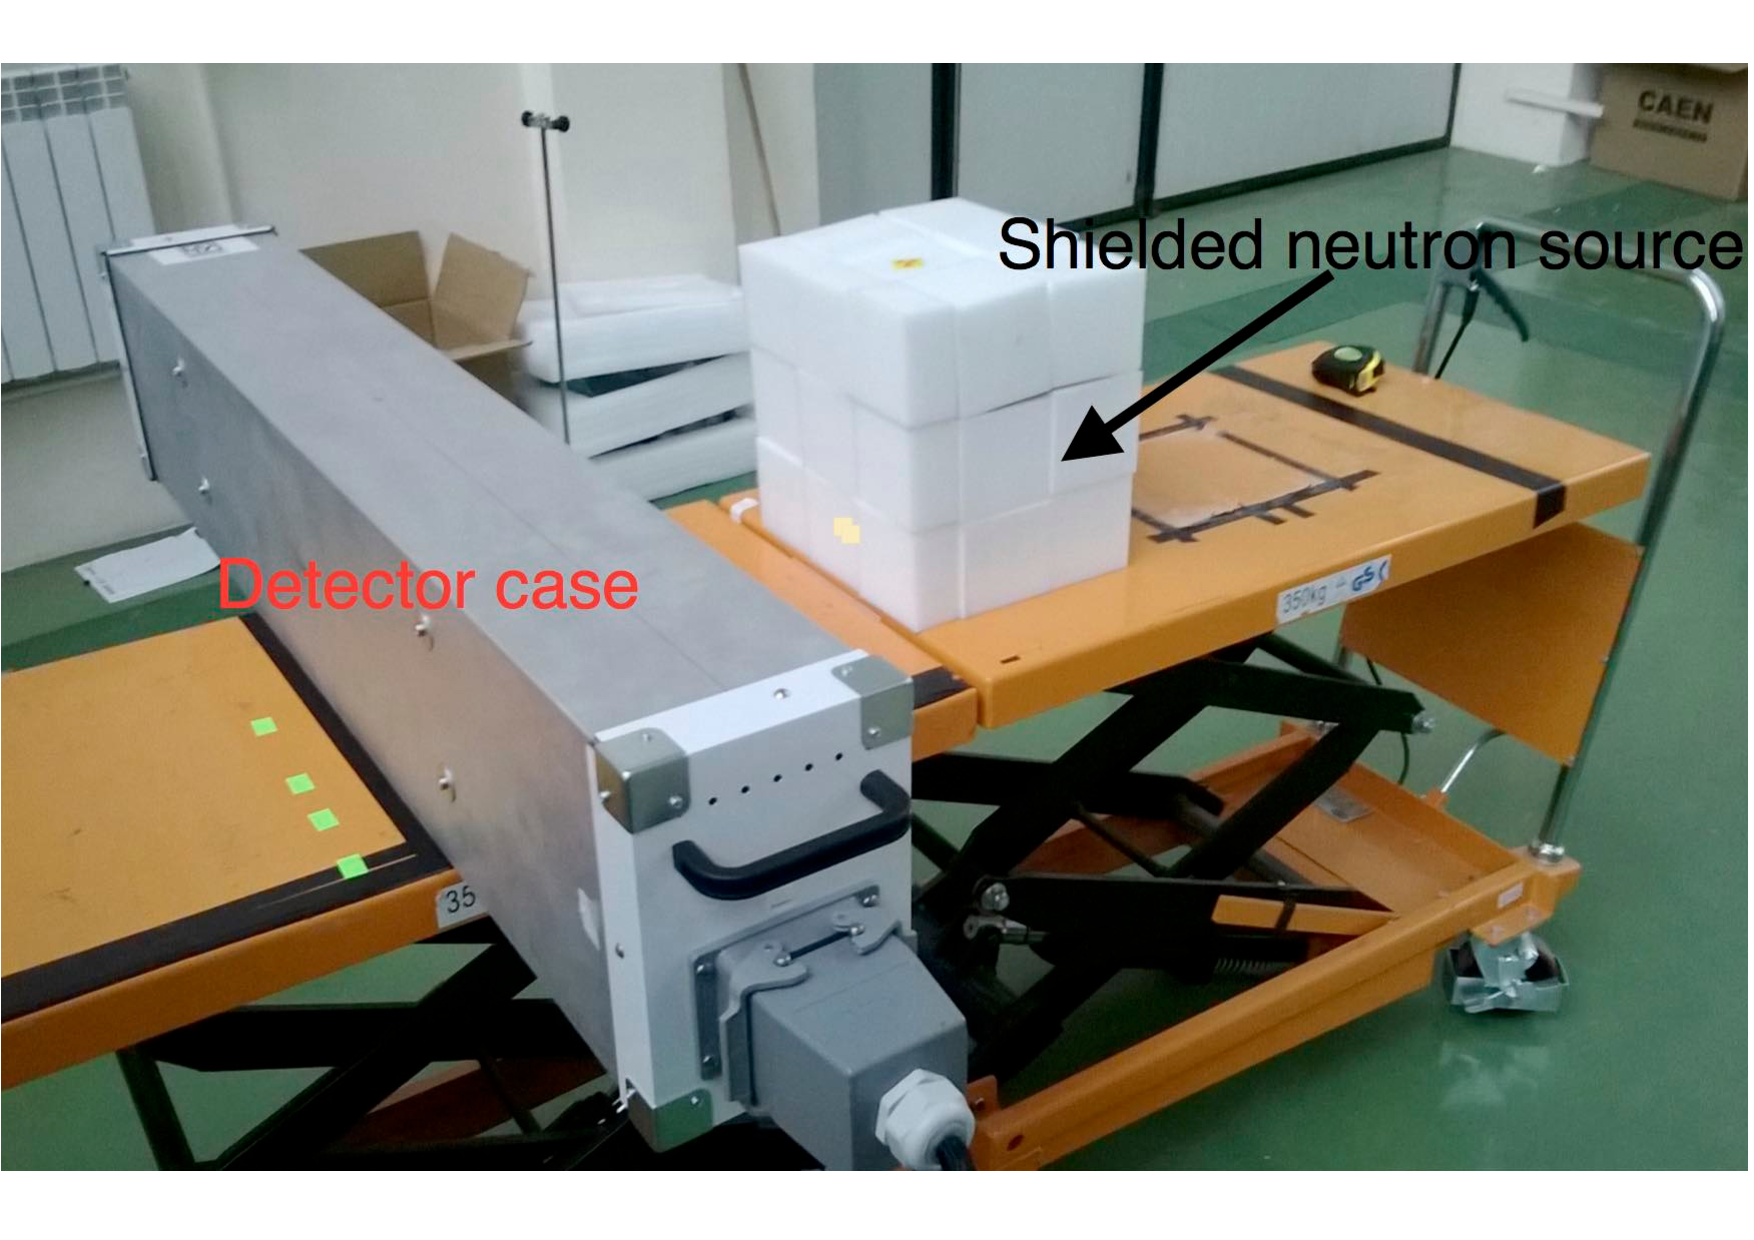
\includegraphics[width=90mm]{Chapter8/figures/cf252ShieldedSource.pdf}
\caption{The shielded $^{252}$Cf source placed inside a polyethylene casing. Plot taken from \cite{modesInternal}.}
\label{fig:thermalNeutronCf252Shielded}
\end{center}
\end{figure}

It was observed that the thermal neutron area in the 2D slow-fast component plot was already quite heavily populated for the unshielded scenario. This heavy background can be attributed to neutron interactions with the detector casing and other apparatus. Taking the ratio of the counts in the populated areas, defined in figure \ref{fig:thermalFastNeutronCut}, for fast and thermal neutrons as $N_{f}$ and $N_{t}$ respectively, we define the quantity $\alpha$ = $N_{t}$/$N_{f}$. This value was determined as $\alpha_{unshielded}$ = (0.20 $\pm$ 0.27) \% for the unshielded case and $\alpha_{shielded}$ = (3.26 $\pm$ 0.18) \% for the shielded case. Using this quantity as the benchmark for whether a source is shielded a reasonable value of $\alpha$ > 0.5 is used to establish this as true \cite{modesInternal}.

\section{Initial System Review}
The MODES-SNM system performed well in the initial tests by surpassing the requirements and showing good stability and reliability in a laboratory environment. However it was obvious that the xenon detector efficiencies at higher energies would need to be improved as this would significantly impair on the system performance and source identification for spectra above 1 MeV. To resolve this issue an additional detector of different technology, a NaI detector, was used to replace the second xenon detector. This has been studied and characterised previously \cite{modesInternal}. The dimensions of this detector are 12.5 $\times$ 12.5 $\times$ 25.0 cm$^{3}$. 

\section{Neutron Gamma Discrimination}
The rest of this chapter focuses on the data collected from the fast neutron detectors only and presents an analysis for neutron-gamma (n-$\gamma$) discrimination, proposed and implemented independently from the MODES-SNM collaboration. Due to this, the following analysis is not implemented in the MODES-SNM prototype system and forms a separate analysis to depict an alternative solution to the problem. It came to light that in the field tests the false alarm rate was quite high and although increasing the threshold is a possible solution, it would decrease sensitivity to radioactive material. The existing discrimination techniques only apply per channel and as a result a fluctuation in one isolated channel will trigger a false alarm whereas a further improvement would be to examine all channels when performing the discrimination. The analysis presented here uses a similar technique to that implemented in the prototype, using a Pulse Shape Discrimination (PSD) technique, but is employed in such a way to make use of all channel data when discriminating between neutrons and gammas. This then aims to improve the n-$\gamma$ discrimination and reduce the false alarm rate that was observed in the field tests.

It is important to discriminate between neutron and gamma events to maximise neutron detection efficiency and reduce the false alarm rate. In this chapter we examine how to discriminate between the two particles using both the fast and slow components of the scintillation light. We have shown that the neutron detectors meet the requirements when a strong neutron source, such as $^{252}$Cf is used, but when gamma sources are used these can trigger a neutron alarm. To combat this issue we use known sources of PuBe, $^{137}$Cs and $^{60}$Co to show the discrimination potential of the fast neutron detectors following various selection procedures. The latter two sources being gamma emitters and PuBe being a strong neutron source.

To motivate the need for particle discrimination a single channel on one neutron detector is used, ignoring the 7 other detectors. Data was collected in a laboratory environment, as previously described earlier in the chapter. However the detectors operating parameters can vary over time, including pressure, temperature and voltages across the PMTs. Both temperature and pressure have an effect on the density of the gas and hence the cross section, which would yield inconsistent event rates. To overcome this dependancy the collected data is normalised to the total number of events collected. Furthermore this also makes the data independent of the source activities. The voltages across the PMTs though do have direct impact on both $Q_{long}$ and $Q_{short}$ values, as it directly affects the charge amplification and charge readout. However the results made available from the tests in Poland were limited and resulted in a severely restricted data set which could be used for the analysis. With limited information on all operating parameters, including voltages, it was not possible to investigate the effect of the voltages on the discrimination power. To overcome this restriction, the processes and algorithms used in this discrimination analysis are designed such that any conclusions and results drawn are to be independent of the operating parameters.
%It is important to identify this effect as if not properly understood, it could potentially reduce the detection capacity of the system as many detectors in practical situations could have differing voltages.

\subsection{Energy Spectra} 
Comparing the energy spectra of the sources measured on the fast neutron detector shows little discrimination between the gamma sources but PuBe is notably different from the gamma sources. Figure \ref{fig:modesSourcesSpectraComparision} shows the $Q_{long}$ value recorded in the fast neutron detector, normalised to the number of events measured in a given time interval. The data collection period of 300 s is chosen to accumulate enough events to reduce statistical errors, at least (1 $\times$ 10$^{6}$ events) for each source. The notable difference between the neutron and gamma sources is clear but shows a large overlap in the spectra at the low energy region, at $\sim$1000 ADC counts. To increase the separation we examine the PSD value of each event.
%However the $^{60}$Co source follows a similar shape to the two neutron sources, thus the $Q_{long}$ value alone cannot discriminate between neutron and gamma sources.

\begin{figure}[htbp]
\begin{center}
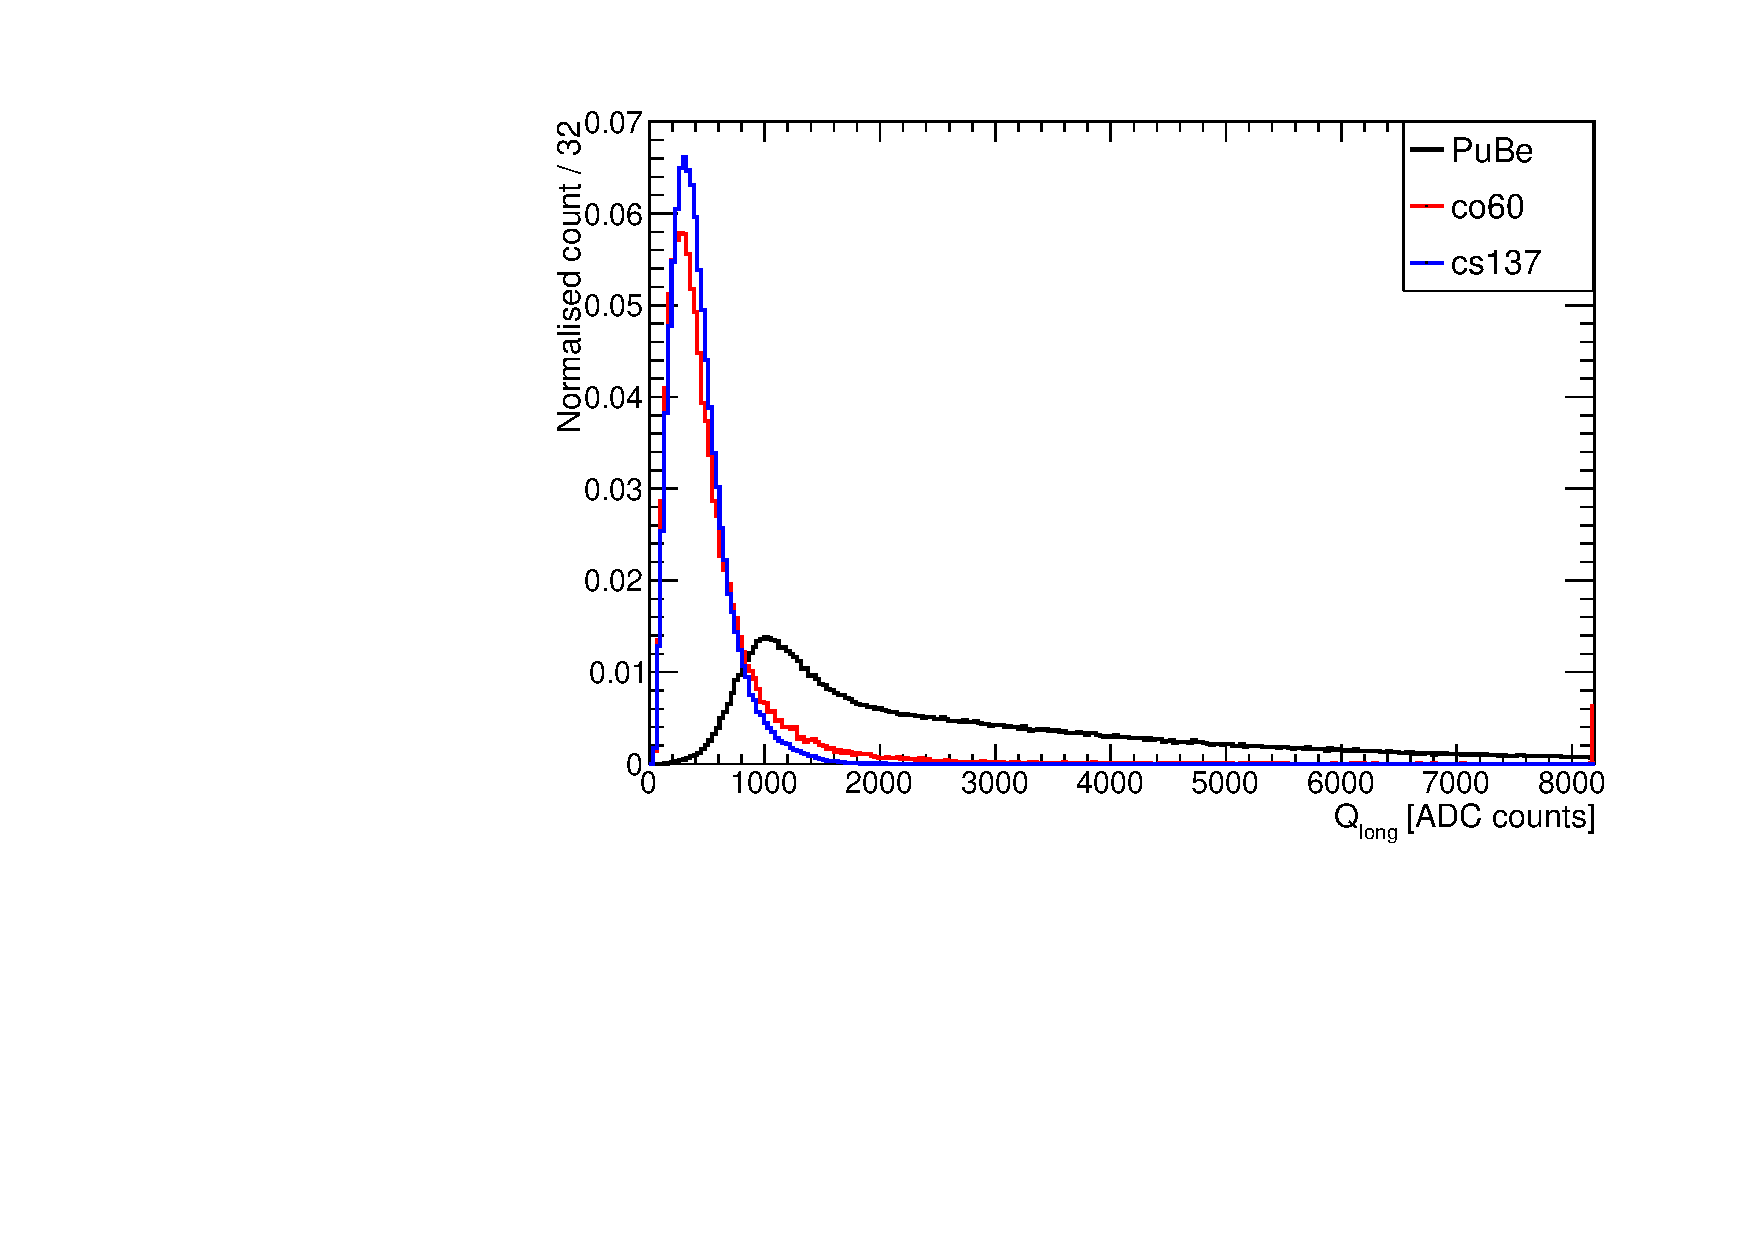
\includegraphics[width=90mm]{Chapter8/figures/spectra_allSources_noCf252_linear.pdf}
\caption{The total integrated charge measured, $Q_{long}$, on channel 0 of one of the fast neutron detectors. Each source is normalised to the number of events recorded - 124148 PuBe events, 589223 $^{60}$Co events and 239418 $^{137}$Cs events. The data used is that corresponding to one channel on one of the fast neutron detectors.}
\label{fig:modesSourcesSpectraComparision}
\end{center}
\end{figure}

\subsection{Pulse Shape Discrimination}
Pulse Shape Discrimination (PSD) methods are an established technique employed by scintillation fast neutron detectors when needing to discriminate against $\gamma$-ray backgrounds. With that very much the case in MODES-SNM it is used as the main method of discrimination between fast neutrons and gammas. If we examine the signal signature of both a neutron and gamma event read by each PMT we can notice clear differences between them, as shown in figure \ref{fig:modesNeutronGammaEventSignals}. For a neutron event the energy deposition occurring from the recoiling nucleus within the gas is spread over a larger time period ($\sim$1.4-2.0$\mu$s) with narrow peaks of charge collection (spikes). Contrary to this the gamma event is typically shorter in its energy deposition ($\sim$0.2-0.4$\mu$s). Thus the PSD value, governed by the difference in the charge collected between the short and long gates, is notably different for each particle.

\begin{figure}[htbp]
\begin{center}
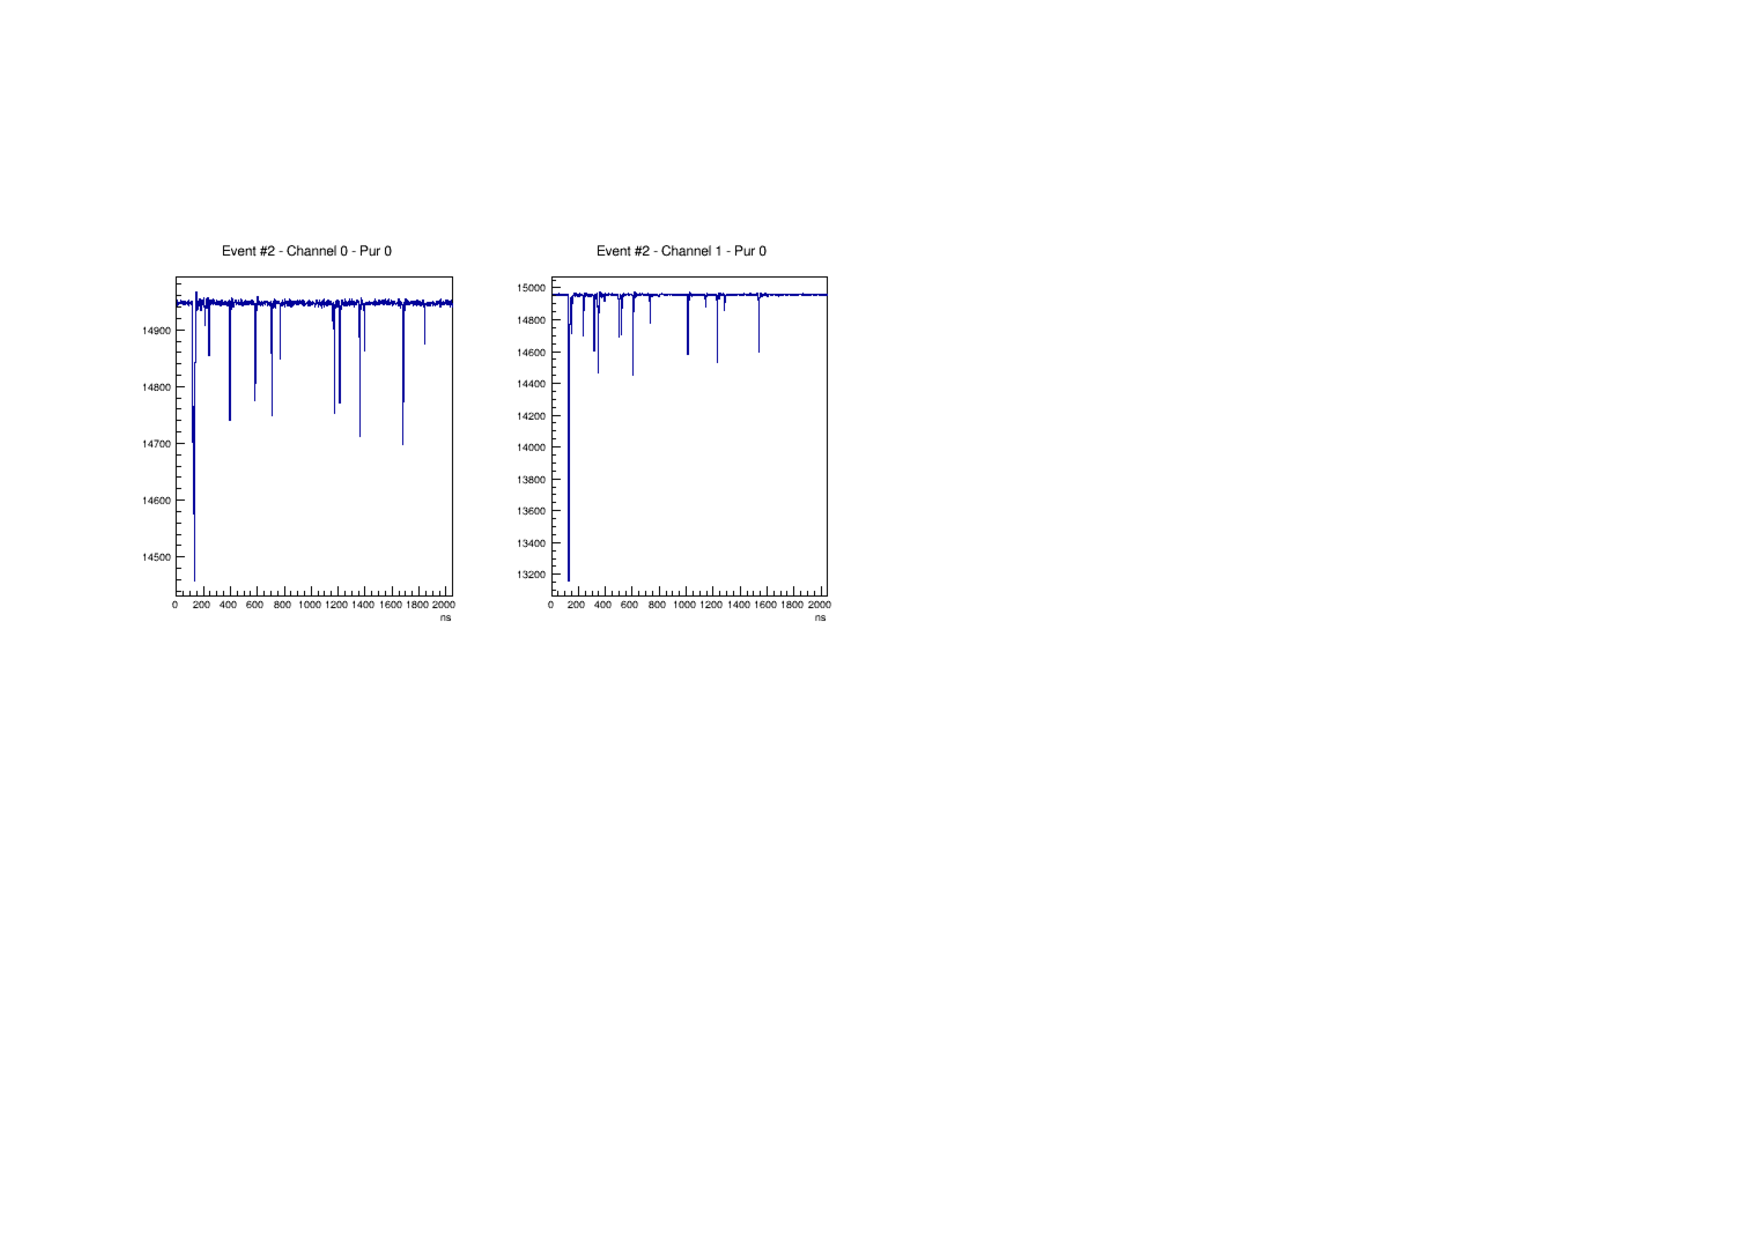
\includegraphics[width=140mm]{Chapter8/figures/fastNeutronEventSignal.pdf} \\
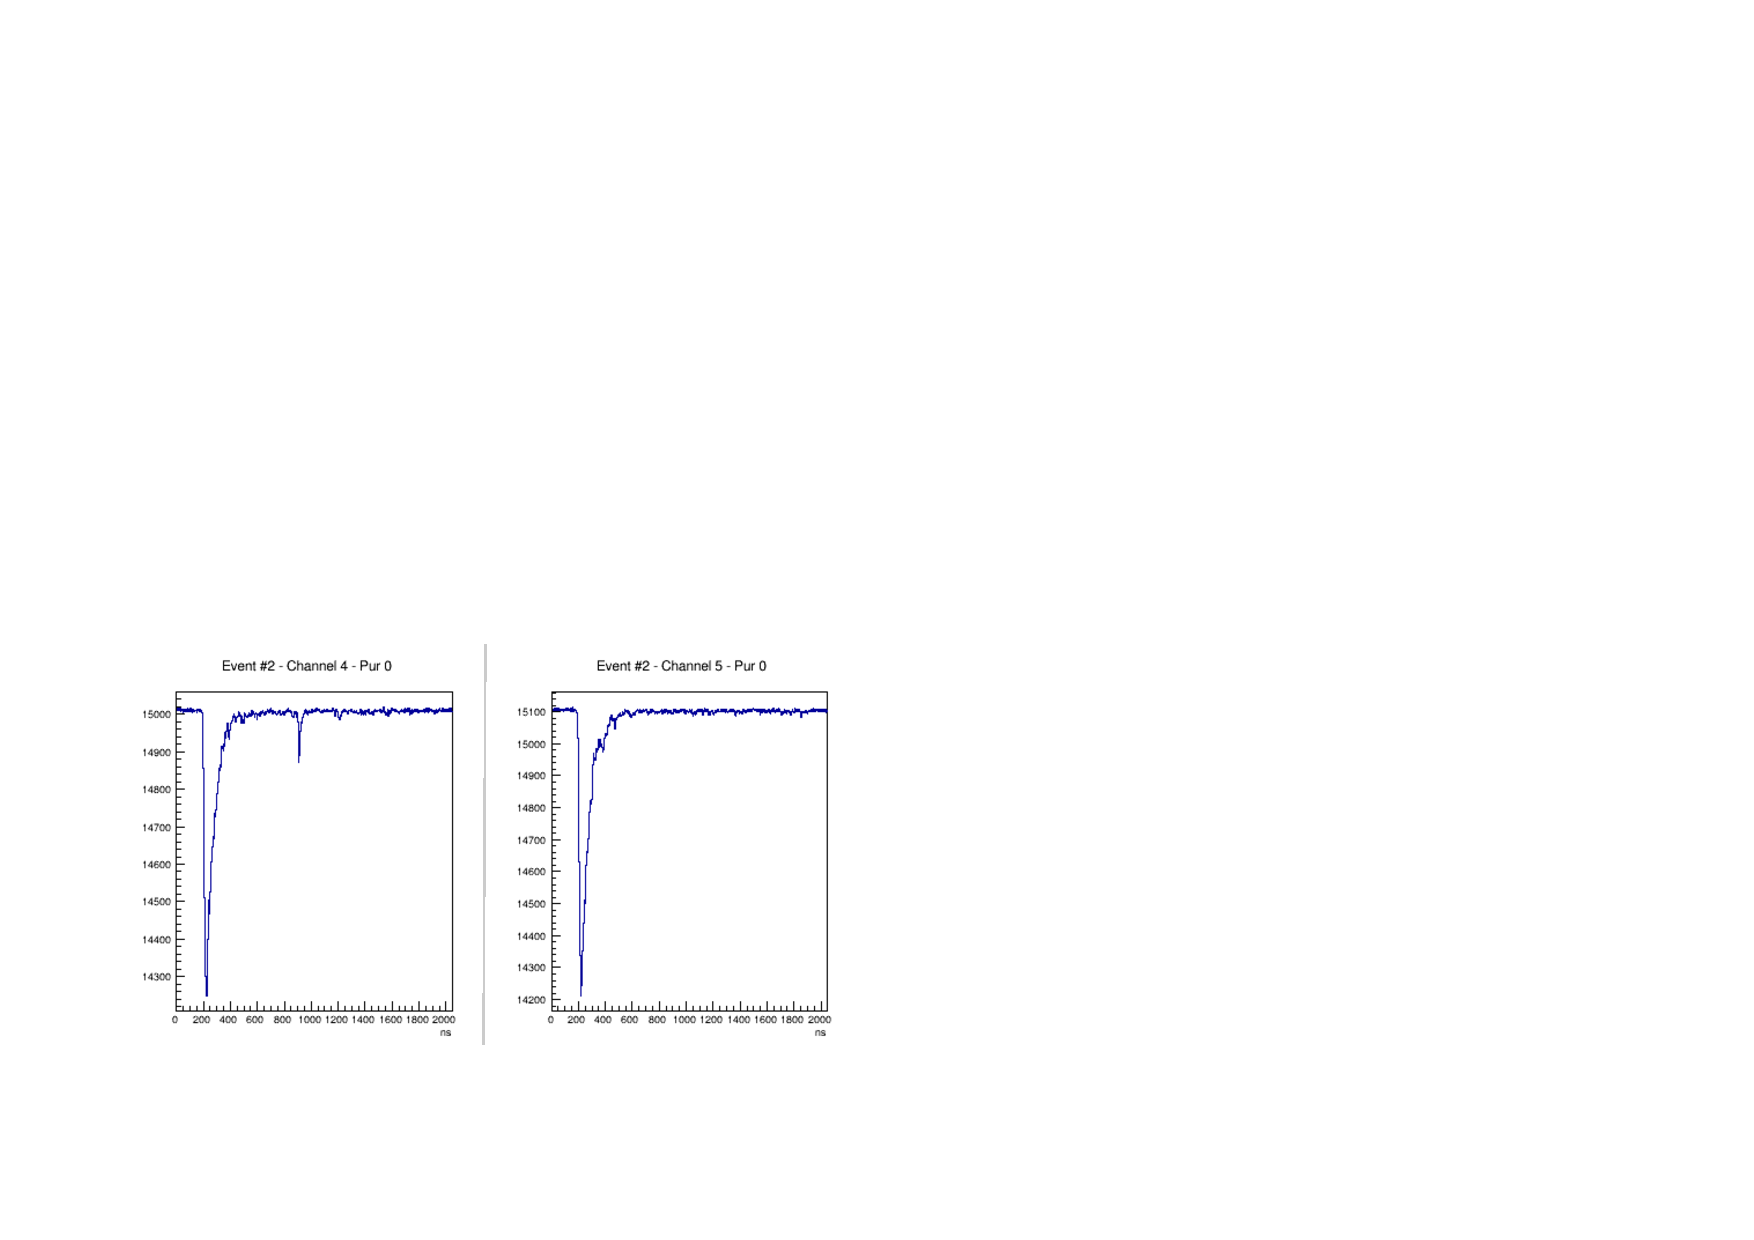
\includegraphics[width=140mm]{Chapter8/figures/gammaEventSignal.pdf} 
\caption{Top: A neutron event recorded by one detector showing the charge as a function of time collected by both detector channels. Bottom: A gamma event recorded by one detector showing the charge as a function of time collected by both detector channels. Figure taken from \cite{modesInternal}.}
\label{fig:modesNeutronGammaEventSignals}
\end{center}
\end{figure}

Using the PSD value the separation between neutron and gamma sources becomes much more apparent than just comparing their spectra, as seen in figure \ref{fig:modesSourcesPSDComparision}. The neutron source has a narrow distribution centred around a high PSD value, at $\sim$0.76, whereas the gamma sources have a broader distribution centred at a lower PSD value of $\sim$0.55. Again each distribution has been normalised to the number of total entries within the data collection period of 300 s. Although the n-$\gamma$ separation is clearer using the PSD value compared to their spectra, there still remains a large area of overlap. To quantify this we introduce the efficiencies, purities and figure of merits to optimise a selection criteria for discriminating between the two particles.

\begin{figure}[htbp]
\begin{center}
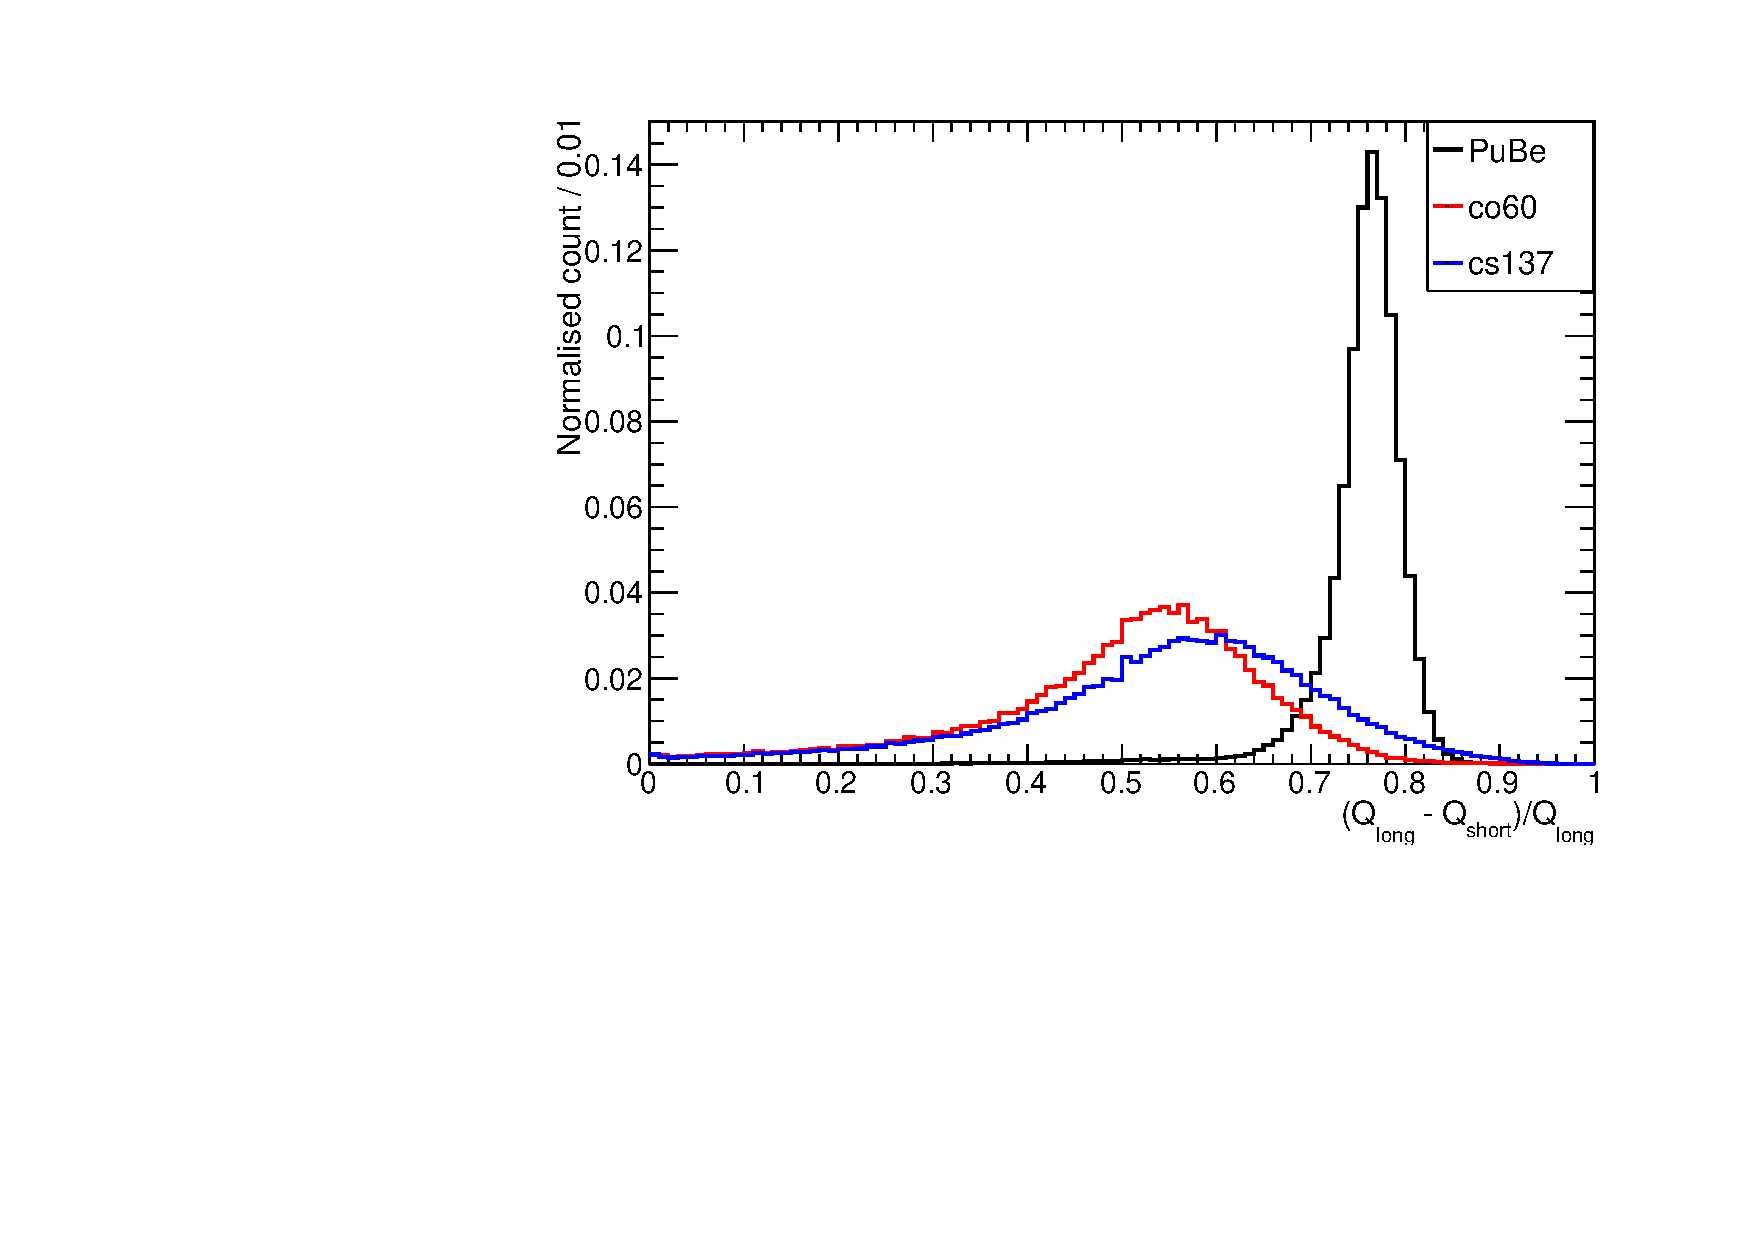
\includegraphics[width=90mm]{Chapter8/figures/psd_allSources_noCf252_linear.pdf}
\caption{The PSD value measured on one channel of one of the fast neutron detectors. Each source is normalised to the number of events recorded - 124148 PuBe events, 589223 $^{60}$Co events and 239418 $^{137}$Cs events. The data used is that corresponding to one channel on one of the fast neutron detectors.}
\label{fig:modesSourcesPSDComparision}
\end{center}
\end{figure}

\subsubsection{Discrimination Optimisation}
Defining the neutron detection efficiency, $\epsilon$, as equation \ref{eq:neutronGammaEff} we impose a selection on the collected events based on the PSD value to optimise the discrimination. Here $n_{i}$ corresponds to the number of entries in the $i^{th}$ bin. A bin width of 0.01 is taken as this provides good granularity while assuring at least one event per bin. Labelling the first bin as 0 includes all binned entries, indicating an efficiency equal to unity, and the final bin as 99 represents the last bin. In this manner the efficiency of the $j^{th}$ bin is determined as a function of the selection, such that $j$=0,1,2,..$N$=99. 

\begin{equation}
\epsilon_{j} = \frac{n_{j}}{n_{0}} = \frac{\sum^{N}_{i=j}{n_{i}}}{\sum^{N}_{i=0}{n_{i}}}
\label{eq:neutronGammaEff}
\end{equation}
The uncertainty associated with $\epsilon_{j}$ is determined using standard binomial treatment of which the uncertainty of the $j^{th}$ bin is given by equation \ref{eq:neutronGammaEffError}.

\begin{equation}
\Delta\epsilon_{j} = \sqrt{\frac{\epsilon_{j}(1 - \epsilon_{j})}{n_{0}}}
\label{eq:neutronGammaEffError}
\end{equation}

In a similar fashion we define the purity, $\eta$, by comparing a signal distribution to a background distribution, in this case a neutron source against a gamma source. The purity of the $j^{th}$ bin is then defined by equation \ref{eq:neutronGammaPurity}, with $n_{i}$ representing the number of signal entries in the $i^{th}$ bin and $l_{i}$ representing the number of background entries in the $i^{th}$ bin. This analysis aims to provide discrimination between neutron and gammas based solely on distribution shape and no information on the source is used other than if it is a neutron or gamma source. Scale factors of $\alpha_{s}$ and $\alpha_{b}$ represent the inverse of the total number of events in the detector due to signal (PuBe) and background ($^{137}$Cs or $^{60}$Co) events. From this definition we can define the purity in terms of their efficiencies, $\epsilon^{s}$ and $\epsilon^{b}$, for signal and background respectively.
%As the number of gammas and neutrons produced per disintegration can vary between sources a 1:1 ratio is assumed between neutrons and gammas.  It should also be noted that in many occasions the particle ratio would not be known.

\begin{equation}
\eta_{j} = \frac{\alpha_{s}\sum^{N}_{i=j}{n_{i}}}{\big(\alpha_{s}\sum^{N}_{i=j}{n_{i}} + \alpha_{b}\sum^{N}_{i=j}{l_{i}} \big)} = 
\frac{\epsilon^{s}_{j}}{\big(\epsilon^{s}_{j} + \epsilon^{b}_{j} \big)}
\label{eq:neutronGammaPurity}
\end{equation}

The uncertainty associated with $\eta_{j}$ follows from the combination of binomial errors from the signal and background efficiencies, given by equation \ref{eq:neutronGammaPurityError}. In limiting cases this can lead to an incorrect treatment of the uncertainties and can provide non physical results. Due to this we impose 0 $< \Delta\eta_{j} <$ 1 and that $\epsilon^{s}_{j} >$ 0.

\begin{equation}
\Delta\eta_{j} = \frac{\eta^{2}_{j}}{\epsilon^{s}_{j}}\sqrt{ \Big( \frac{\epsilon^{b}_{j}}{\epsilon^{s}_{j}} \Big)^{2} (\Delta\epsilon^{s}_{j})^{2} + (\Delta\epsilon^{b}_{j})^{2}  }
\label{eq:neutronGammaPurityError}
\end{equation}

The product of these two parameters, $\lambda = \eta\epsilon$, is then a good indication of the optimal selection criteria and is used as the figure of merit. Figure \ref{fig:modesPSDEffAndPur} shows the comparison of the efficiencies and purities for the neutron source compared with a background gamma source of either $^{137}$Cs or $^{60}$Co. Their figure of merit is also overlaid onto the same plots.

\begin{figure}[htbp]
\begin{center}
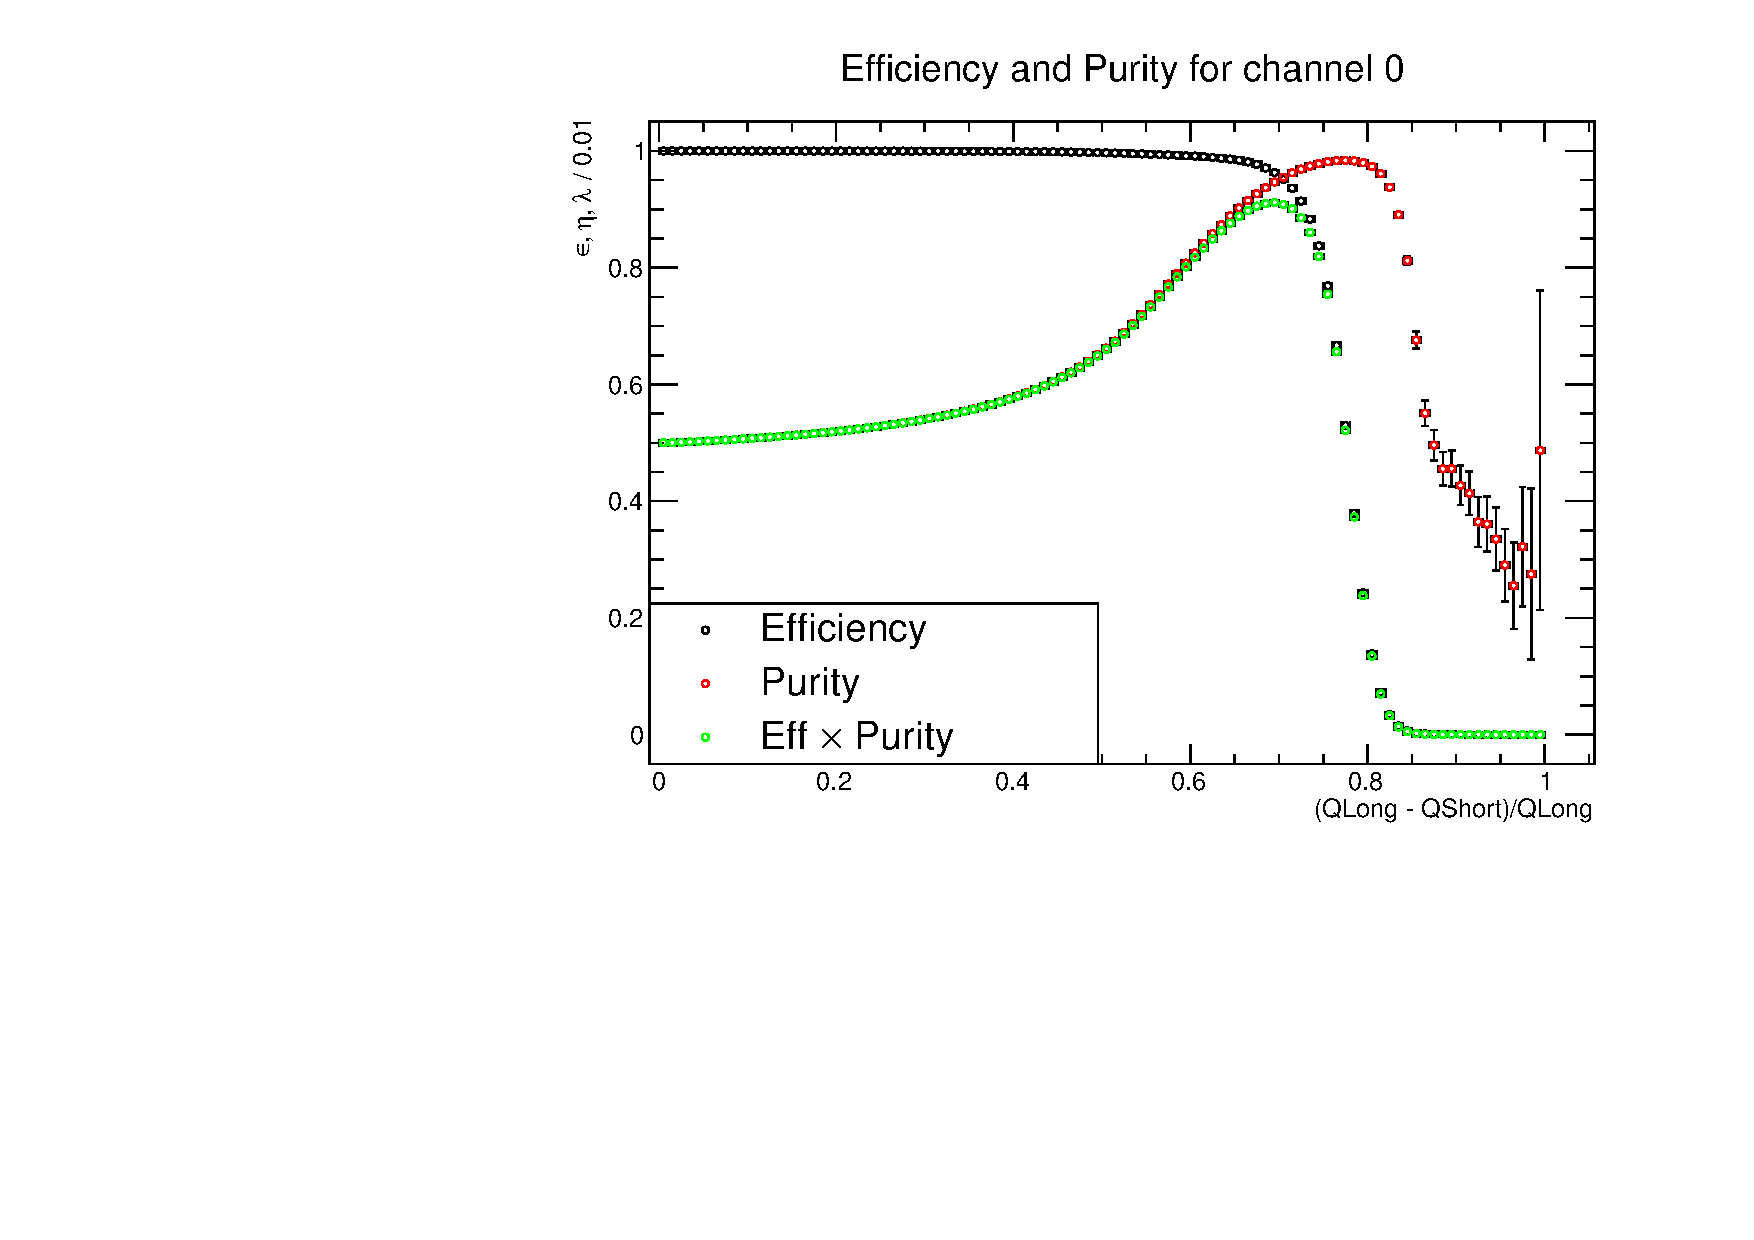
\includegraphics[width=74mm]{Chapter8/figures/eff_pur_pube_co60_errors.pdf}
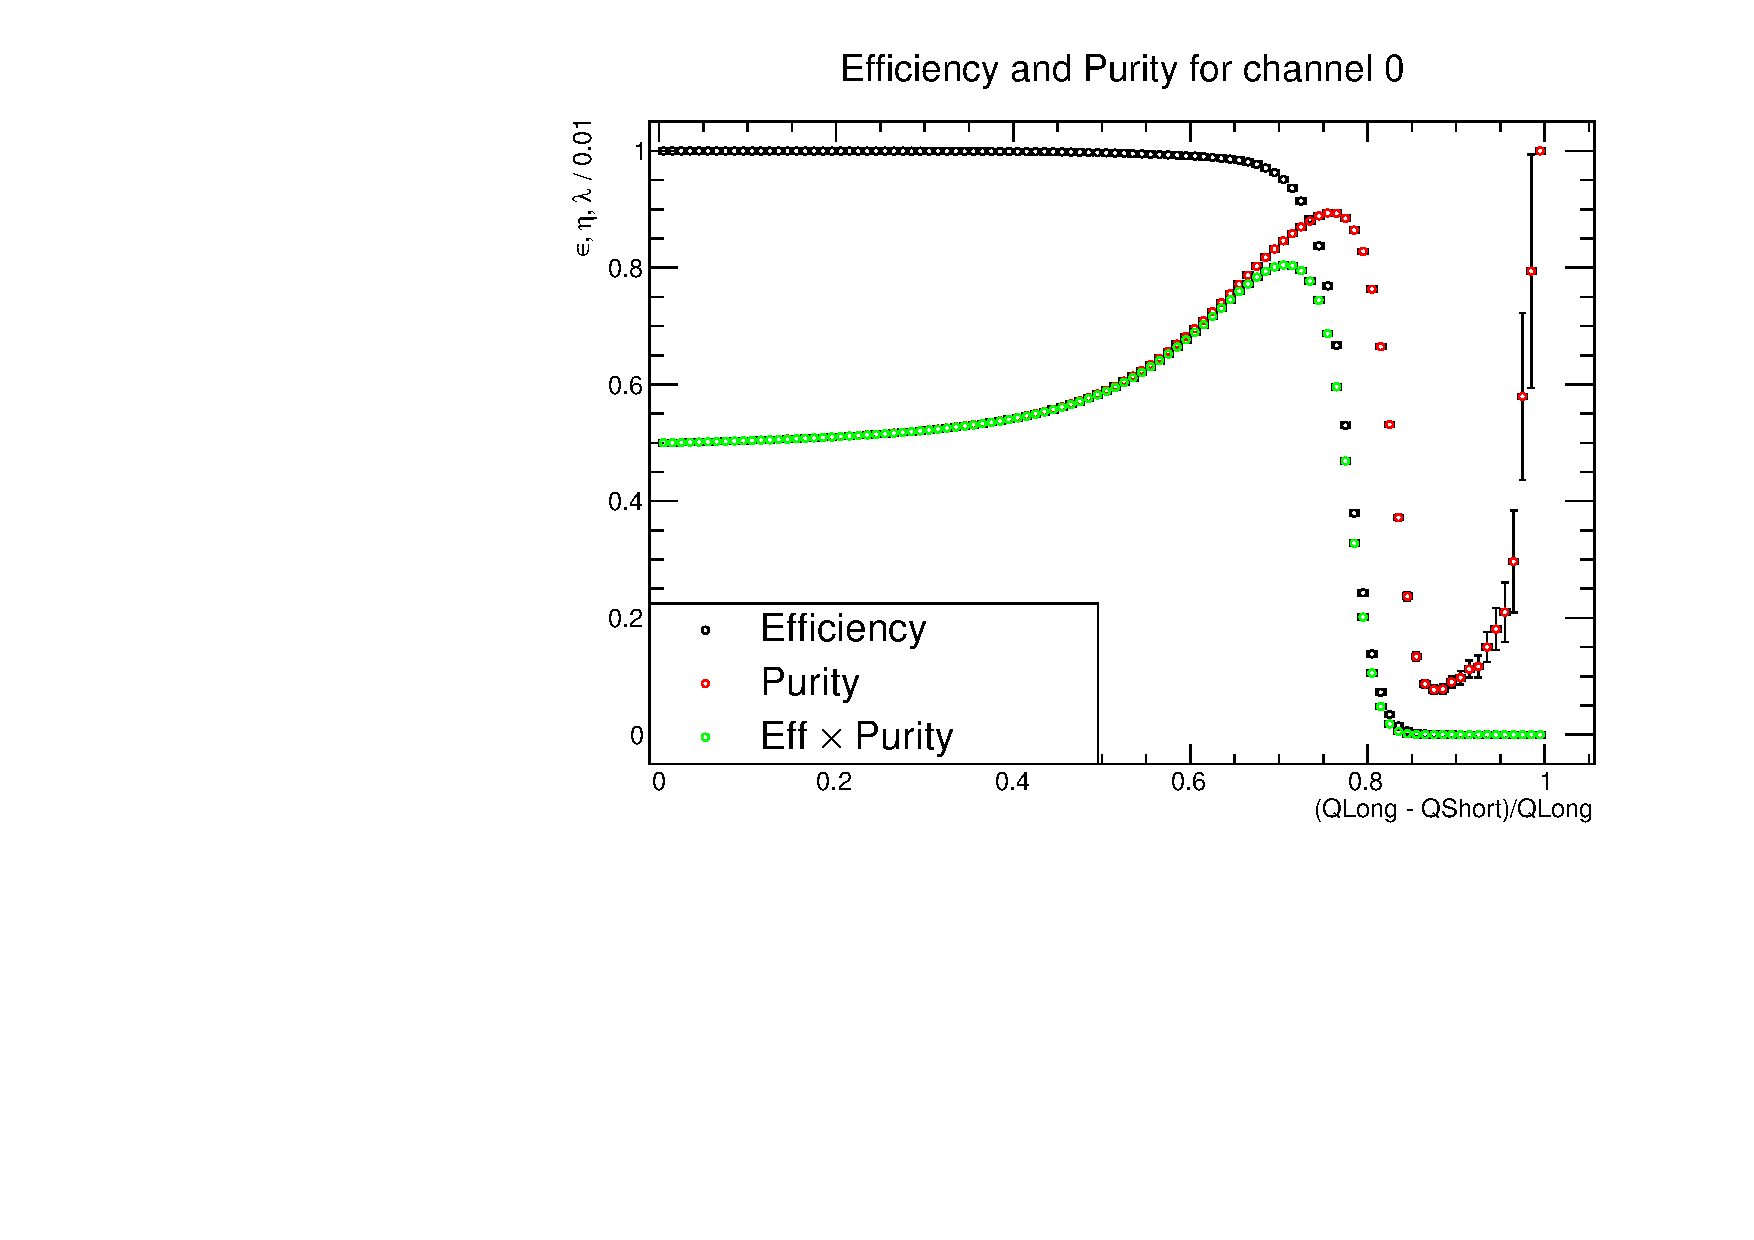
\includegraphics[width=74mm]{Chapter8/figures/eff_pur_pube_cs137_errors.pdf} 
\caption{The efficiencies, purities and figure of merits comparing the neutron source with the gamma sources, PuBe-$^{60}$Co (left) and PuBe-$^{137}$Cs (right). The data used is that corresponding to channel 0 on one of the fast neutron detectors.}
\label{fig:modesPSDEffAndPur}
\end{center}
\end{figure}

The highest figure of merit values for each of the two plots can be seen in table \ref{tab:modesPSDBestCuts}. Both comparisons showed fairly consistent values for the optimal selection value, at 0.695 $\pm$ 0.005 and 0.705 $\pm$ 0.005. However the figure of merit values are relatively different with PuBe/$^{60}$Co at $\lambda_{max}$ = 0.9118 $\pm$ 0.0006 and PuBe/$^{60}$Co at $\lambda_{max}$ = 0.8046 $\pm$ 0.0007. This is due to the larger tail in the $^{137}$Cs distribution which could be due to the lower energy photons having a smaller slow scintillation component. For the MODES system to be able to discriminate between neutrons and gammas at a level to match the system requirements, these values need to be vastly improved.
\begin{table}[h]
\centering
	\begin{tabular}{lcccc}
	\hline
	\textbf{Source} & \textbf{Background} &{$\mathbf{\lambda_{max}}$} & \textbf{Best PSD cut value} \\
	\hline
	PuBe & $^{60}$Co & 0.9118 $\pm$ 0.0006 & 0.695 $\pm$ 0.005\\ 
	PuBe & $^{137}$Cs& 0.8046 $\pm$ 0.0007 & 0.705 $\pm$ 0.005\\ 
	\hline
\end{tabular}
\caption{A table showing the best cut on the PSD value to yield the highest figure of merit, $\lambda_{max}$, for PuBe against each of the two gamma sources. }
\label{tab:modesPSDBestCuts}
\end{table}

\subsubsection{Multiple Channels}
Up until now we have examined only a single channel on one of the fast neutron detectors, using a long data capture time window of 300 seconds. However in reality such a time window would be unachievable and far lower times are to be expected, $\sim$2 seconds. Therefore it is beneficial to combine data collected from multiple detectors to increase statistics while also achieving a larger coverage area. This can be useful if the source is partially shielded or directed differently. 

For the MODES-SNM system prototype 8 fast neutron detectors are to be used, however at the time of testing only 4 detectors were available for data collection, totalling to 8 channels. If we examine the raw data collected for the PuBe and $^{60}$Co sources it can be noticed that there is a large variation between each channel in both amount of events collected and distribution shape. Figures \ref{fig:modesQLongAllChannelsRaw} and \ref{fig:modesQShortAllChannelsRaw} show the long and short components of the integrated charge collected at each channel with the neutron source in black and the gamma source in red. Again the distributions have been normalised to the number of events collected. No restrictions or selections are imposed on the collected events with the figures showing only raw data. Each two consecutive channels (0\&1, 2\&3, 4\&5,  6\&7) represent one detector. 

\begin{figure}[htbp]
\begin{center}
%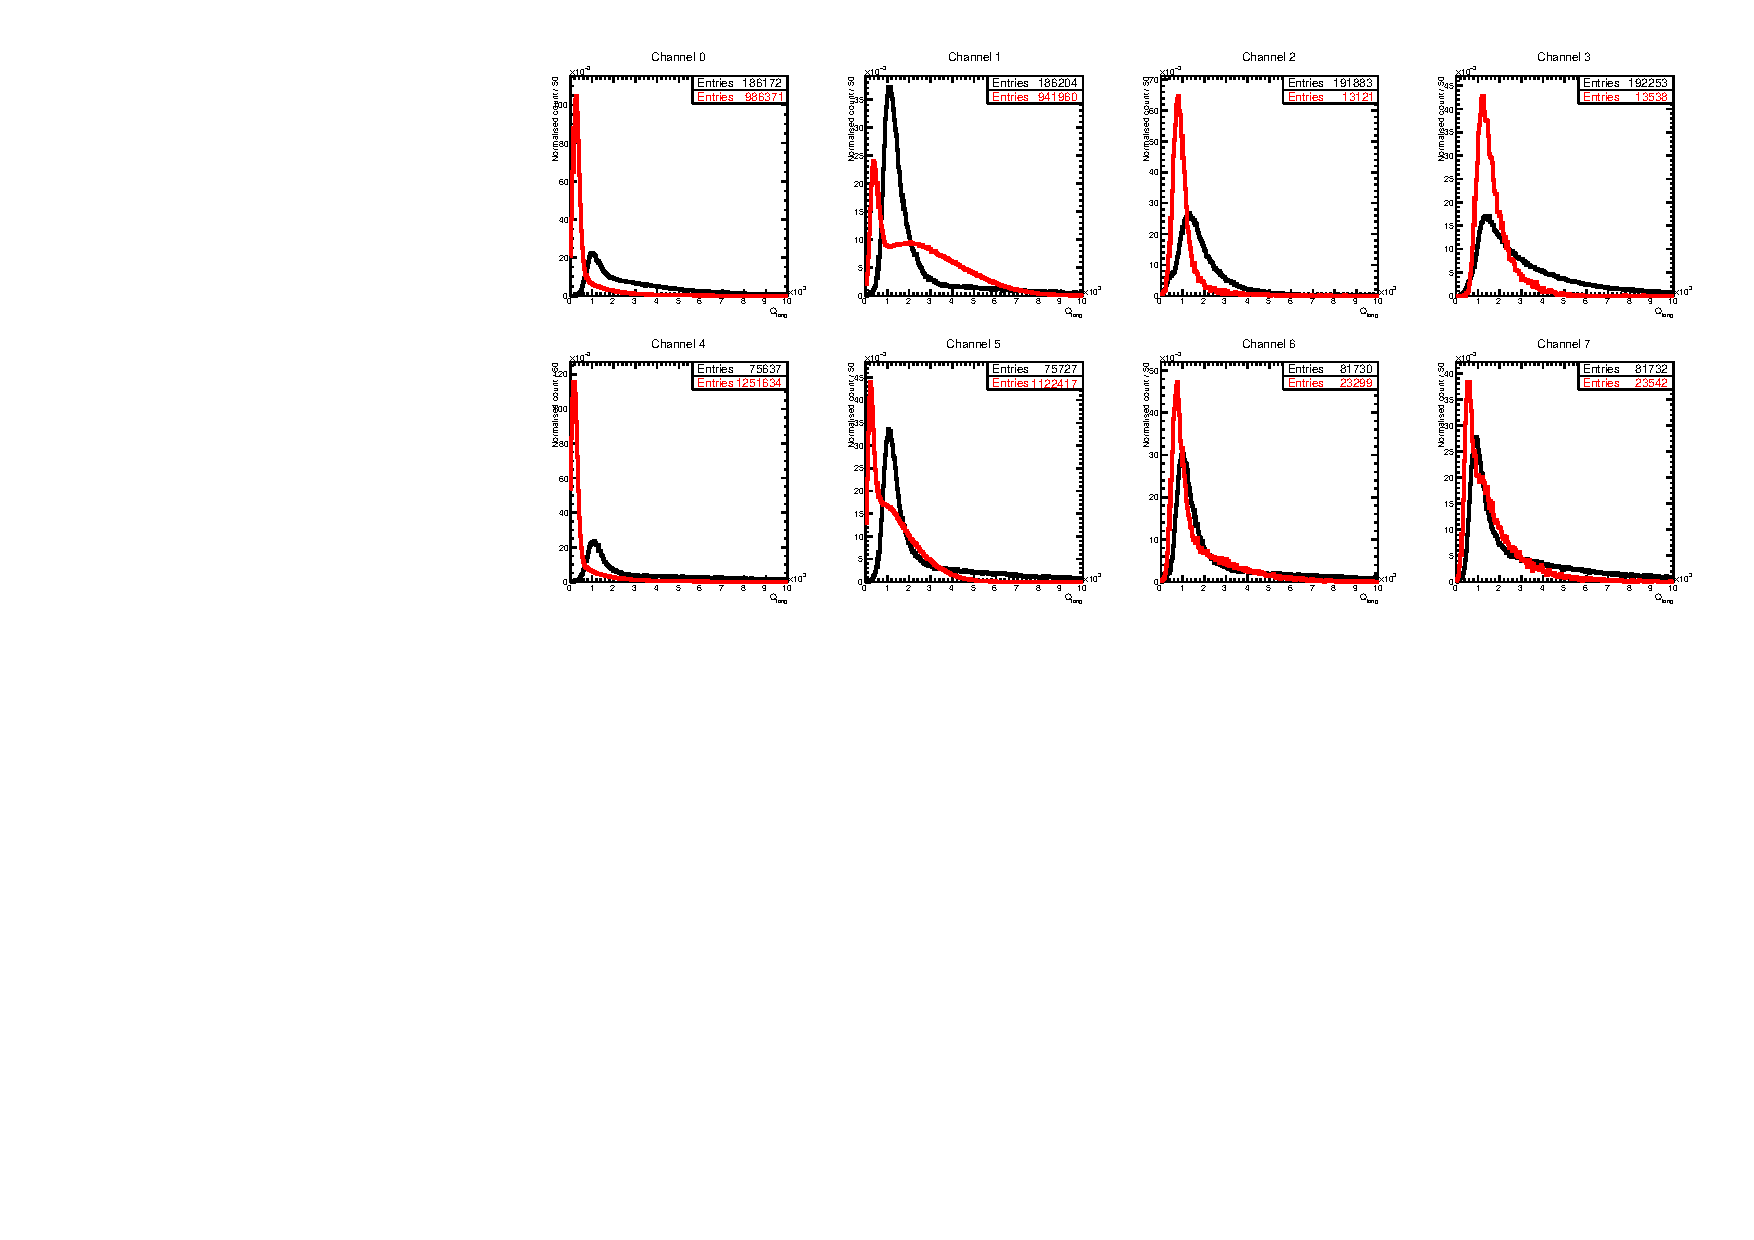
\includegraphics[width=160mm]{Chapter8/figures/QLong_allChannels_pube_co60_noPeaks_rawData.pdf}
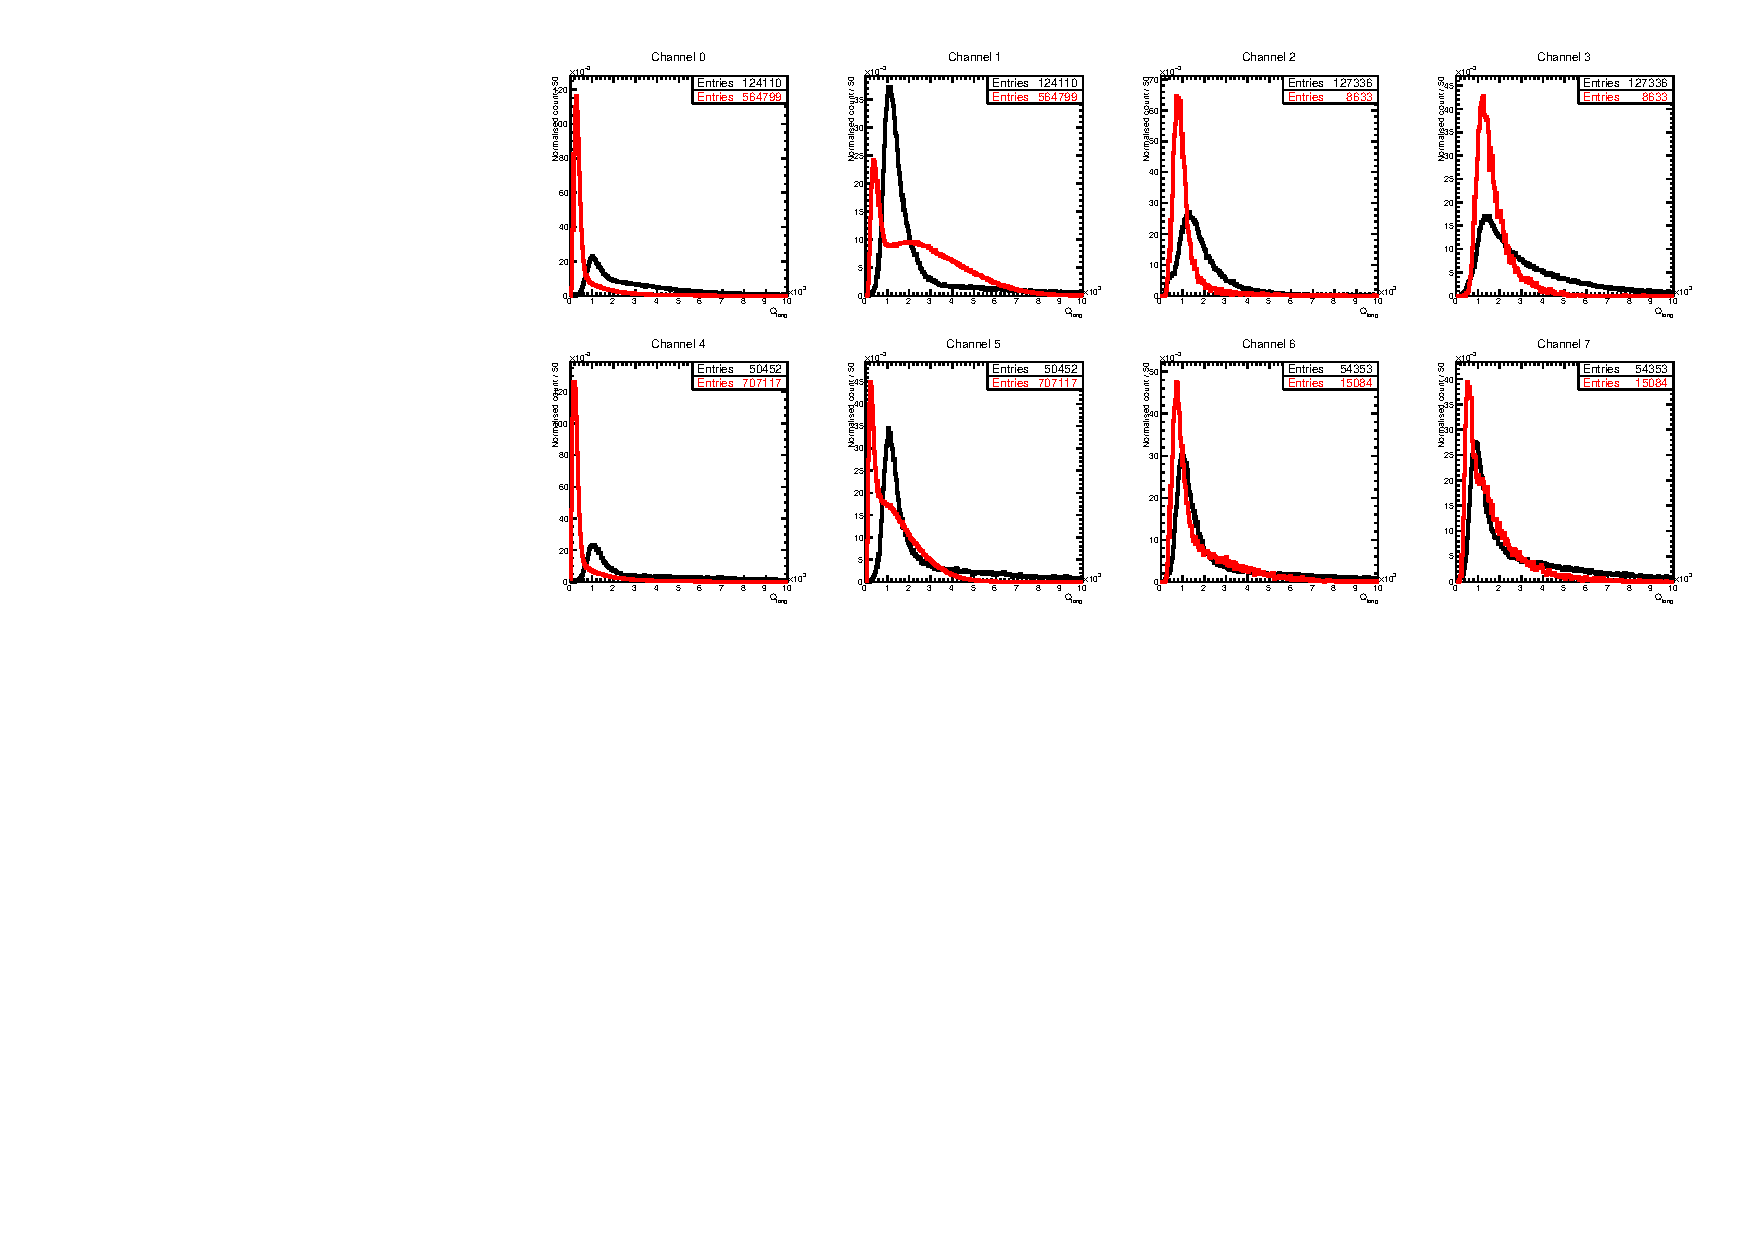
\includegraphics[width=160mm]{Chapter8/figures/QLong_allChannels_pube_co60.pdf}
\caption{The total integrated charge measured, $Q_{long}$, on 4 fast neutron detectors (8 channels) for a PuBe neutron source (black line) and a $^{60}$Co gamma source (red line). Each source is normalised to the number of events recorded in that channel and no restrictions or selections are imposed on the collected events. }
\label{fig:modesQLongAllChannelsRaw}
\end{center}
\end{figure}

\begin{figure}[htbp]
\begin{center}
%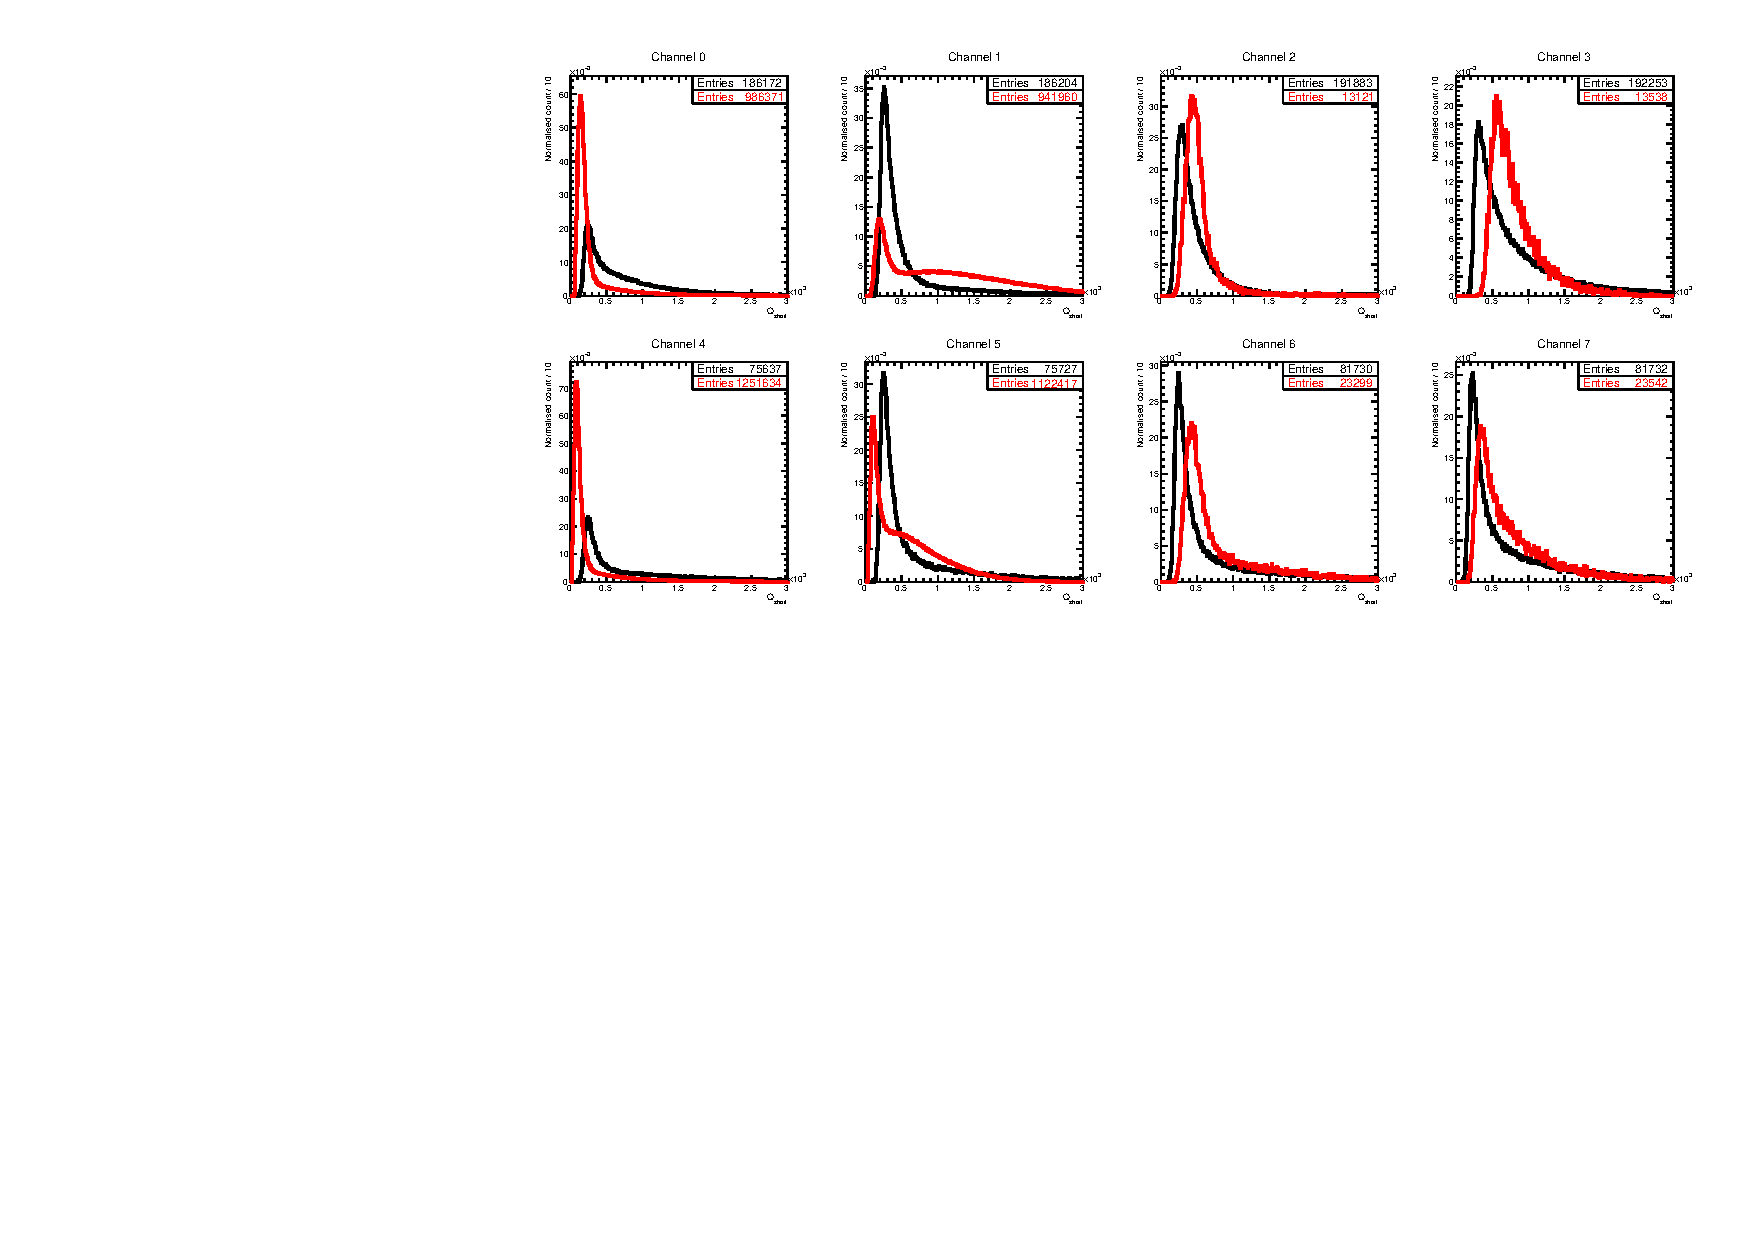
\includegraphics[width=160mm]{Chapter8/figures/QShort_allChannels_pube_co60_noPeaks_rawData.pdf}
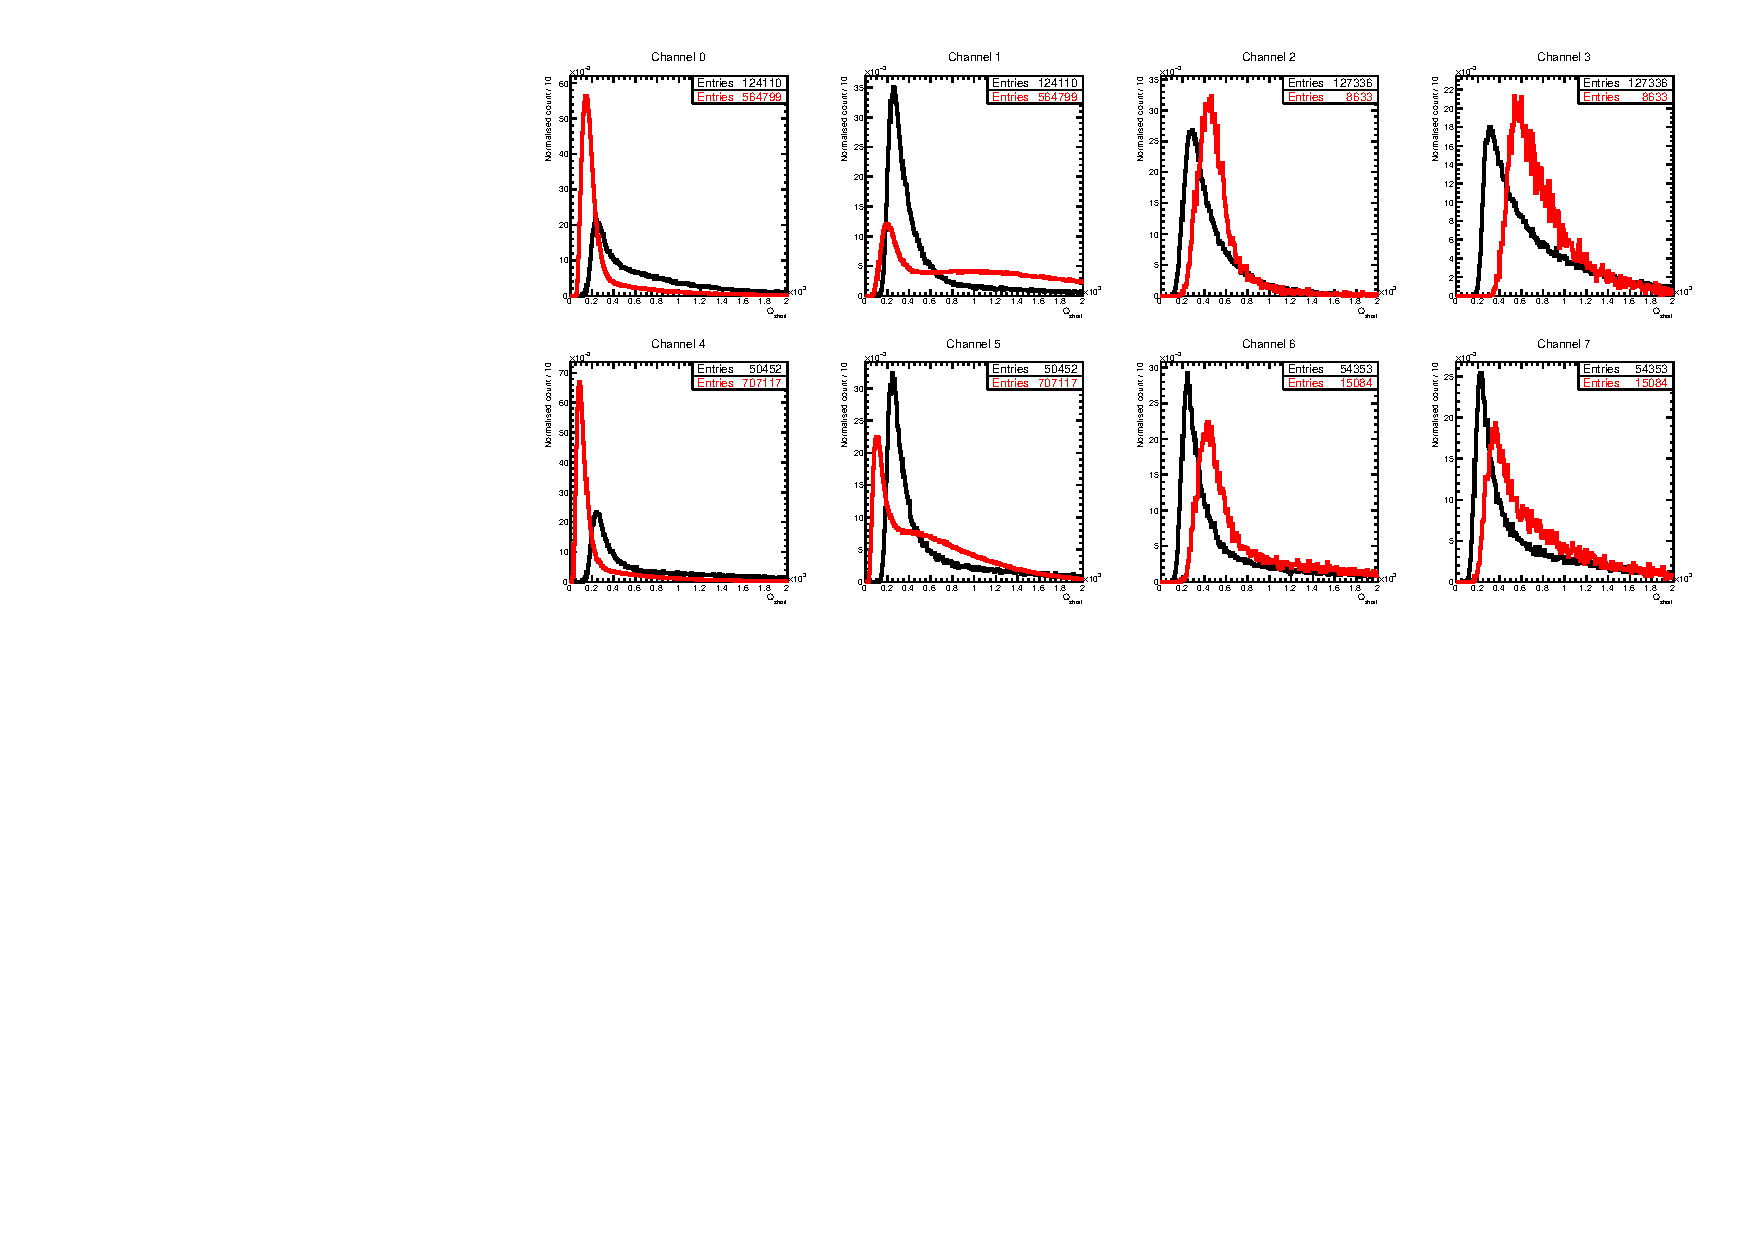
\includegraphics[width=160mm]{Chapter8/figures/QShort_allChannels_pube_co60.pdf}
\caption{The integrated charge measured in the short gate, $Q_{short}$, on 4 fast neutron detectors (8 channels) for a PuBe neutron source (black line) and a $^{60}$Co gamma source (red line). Each source is normalised to the number of events recorded in that channel and no restrictions or selections are imposed on the collected events.}
\label{fig:modesQShortAllChannelsRaw}
\end{center}
\end{figure}

The largest difference in events can be seen between detectors 1 and 3, channels 0\&1 and 4\&5 respectively, for the neutron source with the latter recording $\sim$2.5 times less events. For the gamma source the difference is much larger but detectors 1 and 3 having considerable more events than detectors 2 and 4, a factor of $\sim$85 between detectors 2 and 3. In both cases this is most likely due to the placement of the source with respect to the arrangement of the detector arrays. As detectors 1 and 2 are housed in the same box (box 1), as are detectors 3 and 4 (box 2), when the data was collected for the neutron source, box 1 was most likely placed closer to the neutron source with box 2 directly behind box 1. This would then explain why the events are similar across detectors 1 and 2 and detectors 3 and 4. However the setup for the gamma data collection is likely to have differed such that the boxes were placed together with the source placed on top of both boxes. This would then shield the lower detectors and heavily reduce the gamma events incident on the lower detectors. The arrangement of the detector boxes in the prototype system would need to optimise the positions such that large coverage can be achieved while maintaining high statistics for both neutrons and gammas. For the purpose of this analysis, the difference in the number of events across detectors is not an issue as each channel is normalised to the number of events per channel. However imposing the same number of events per detector should be included to reduce detector noise.

The variation in the distributions across the channels is most noticeable between channels 0 and 1, for both long and short components. Both of these channels represent the same detector yet channel 1 has a large amount of noise, showing a second peak at higher charge. 
%Why does this occur? -This originates from the short component of the charge collection due to......

Examining the PSD values removes the noise and shows a stronger correlation between the distributions, as can be seen in figure \ref{fig:modesPSDAllChannelsRaw}. Each distribution follows a similar shape for both neutrons and gammas and a Gaussian peak is fitted to each channel PSD distribution. By fitting a Gaussian function to within 70\% of the peak value using a $\chi^{2}$ /$n.d.f$ best fit allows each channel to be quantified. The fit parameters are shown in the figure and are summarised in table \ref{tab:modesPSDAllChannelsRawValues}. The requirement of having the same number of events in a single detector tube, is also enforced in the PSD distributions.
 
\begin{figure}[htbp]
\begin{center}
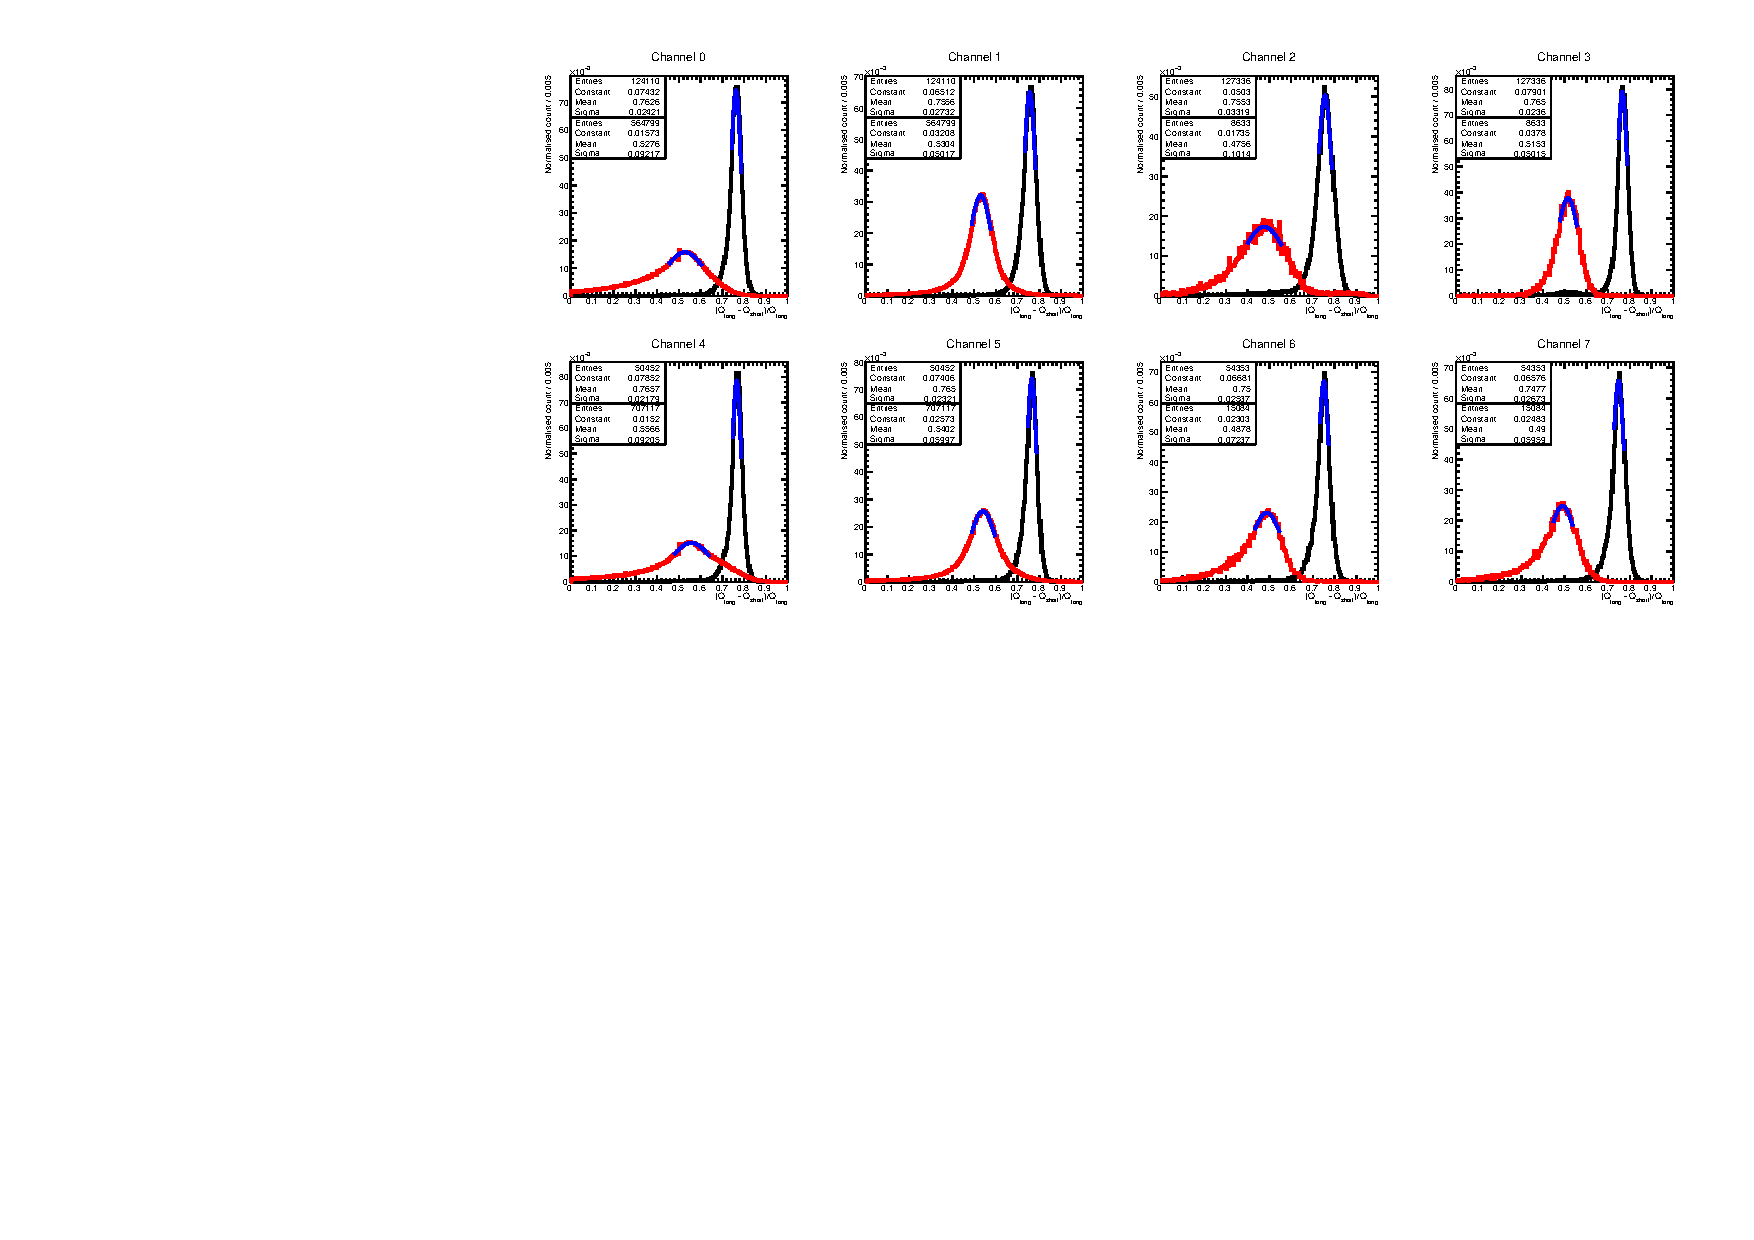
\includegraphics[width=160mm]{Chapter8/figures/psd_allChannels_pube_co60_withPeaksAndCutsAndNoShift.pdf}
\caption{The PSD distributions measured on 4 fast neutron detectors (8 channels) for a PuBe neutron source (black) and a $^{60}$Co gamma source (red). Each source is normalised to the number of events recorded in that channel and is fitted with a Gaussian distribution on the PSD peak value.}
\label{fig:modesPSDAllChannelsRaw}
\end{center}
\end{figure}

\begin{table}[h]
\centering
	\begin{tabular}{ccccc}
	\hline
	& \multicolumn{2}{c}{\textbf{Mean value} ($\mathbf{\bar{x}}$)} & \multicolumn{2}{c}{\textbf{Sigma value} ($\mathbf{\sigma}$)} \\
	\textbf{Channel} & \textbf{PuBe} & \textbf{$^{60}$Co} & \textbf{PuBe} & \textbf{$^{60}$Co} \\
	\hline
	0  & 0.7626 $\pm$ 0.0002 & 0.5276 $\pm$ 0.0004 & 0.0228 $\pm$ 0.0003 & 0.0915 $\pm$ 0.0008\\ 
	1  & 0.7556 $\pm$ 0.0002 & 0.5304 $\pm$ 0.0002 & 0.0258 $\pm$ 0.0003 & 0.0492 $\pm$ 0.0003\\ 
	2  & 0.7553 $\pm$ 0.0002 & 0.4760 $\pm$ 0.0030 & 0.0320 $\pm$ 0.0004 & 0.1000 $\pm$ 0.0080\\ 
	3  & 0.7650 $\pm$ 0.0001 & 0.5150 $\pm$ 0.0020 & 0.0220 $\pm$ 0.0003 & 0.0490 $\pm$ 0.0030\\ 
	4  & 0.7657 $\pm$ 0.0002 & 0.5566 $\pm$ 0.0003 & 0.0202 $\pm$ 0.0003 & 0.0921 $\pm$ 0.0007\\ 
	5  & 0.7650 $\pm$ 0.0002 & 0.5402 $\pm$ 0.0002 & 0.0216 $\pm$ 0.0004 & 0.0593 $\pm$ 0.0004\\ 
	6  & 0.7500 $\pm$ 0.0003 & 0.4880 $\pm$ 0.0020 & 0.0236 $\pm$ 0.0006 & 0.0710 $\pm$ 0.0040\\ 
	7  & 0.7477 $\pm$ 0.0003 & 0.4900 $\pm$ 0.0020 & 0.0250 $\pm$ 0.0005 & 0.0590 $\pm$ 0.0040\\ 
	\hline
\end{tabular}
\caption{A table showing the parameters and their uncertainties of the Gaussian function fitted to the peak value on the PSD distribution for PuBe and $^{60}$Co sources.}
\label{tab:modesPSDAllChannelsRawValues}
\end{table}

From examination of the mean values presented in table \ref{tab:modesPSDAllChannelsRawValues} it is apparent that the values are not consistent with each other when using the fit errors. The mean values across the channels are 0.758 and 0.51 for PuBe and $^{60}$Co respectively. By taking the variance of this mean value, $\bar{x_{0}}$, across the 8 channels yields a considerable difference between the two sources, 0.007 and 0.03 for PuBe and $^{60}$Co respectively. When examining the channels within the same detector the mean PSD values differ less, suggesting that the differences occur due to the detector properties (pressure differences of the gas), playing a larger factor than variance in PMT properties, such as voltage. The uncertainties associated with the fit values represent that of the fit alone and their low values highlight how well the fit represent the peaks. If the standard deviation, $\sigma$, values from the Gaussian fits are used to represent the uncertainty of the means then it is clear the results are fairly consistent, as shown in figure \ref{fig:modesPSDMeanForChannels}.

\begin{figure}[htbp]
\begin{center}
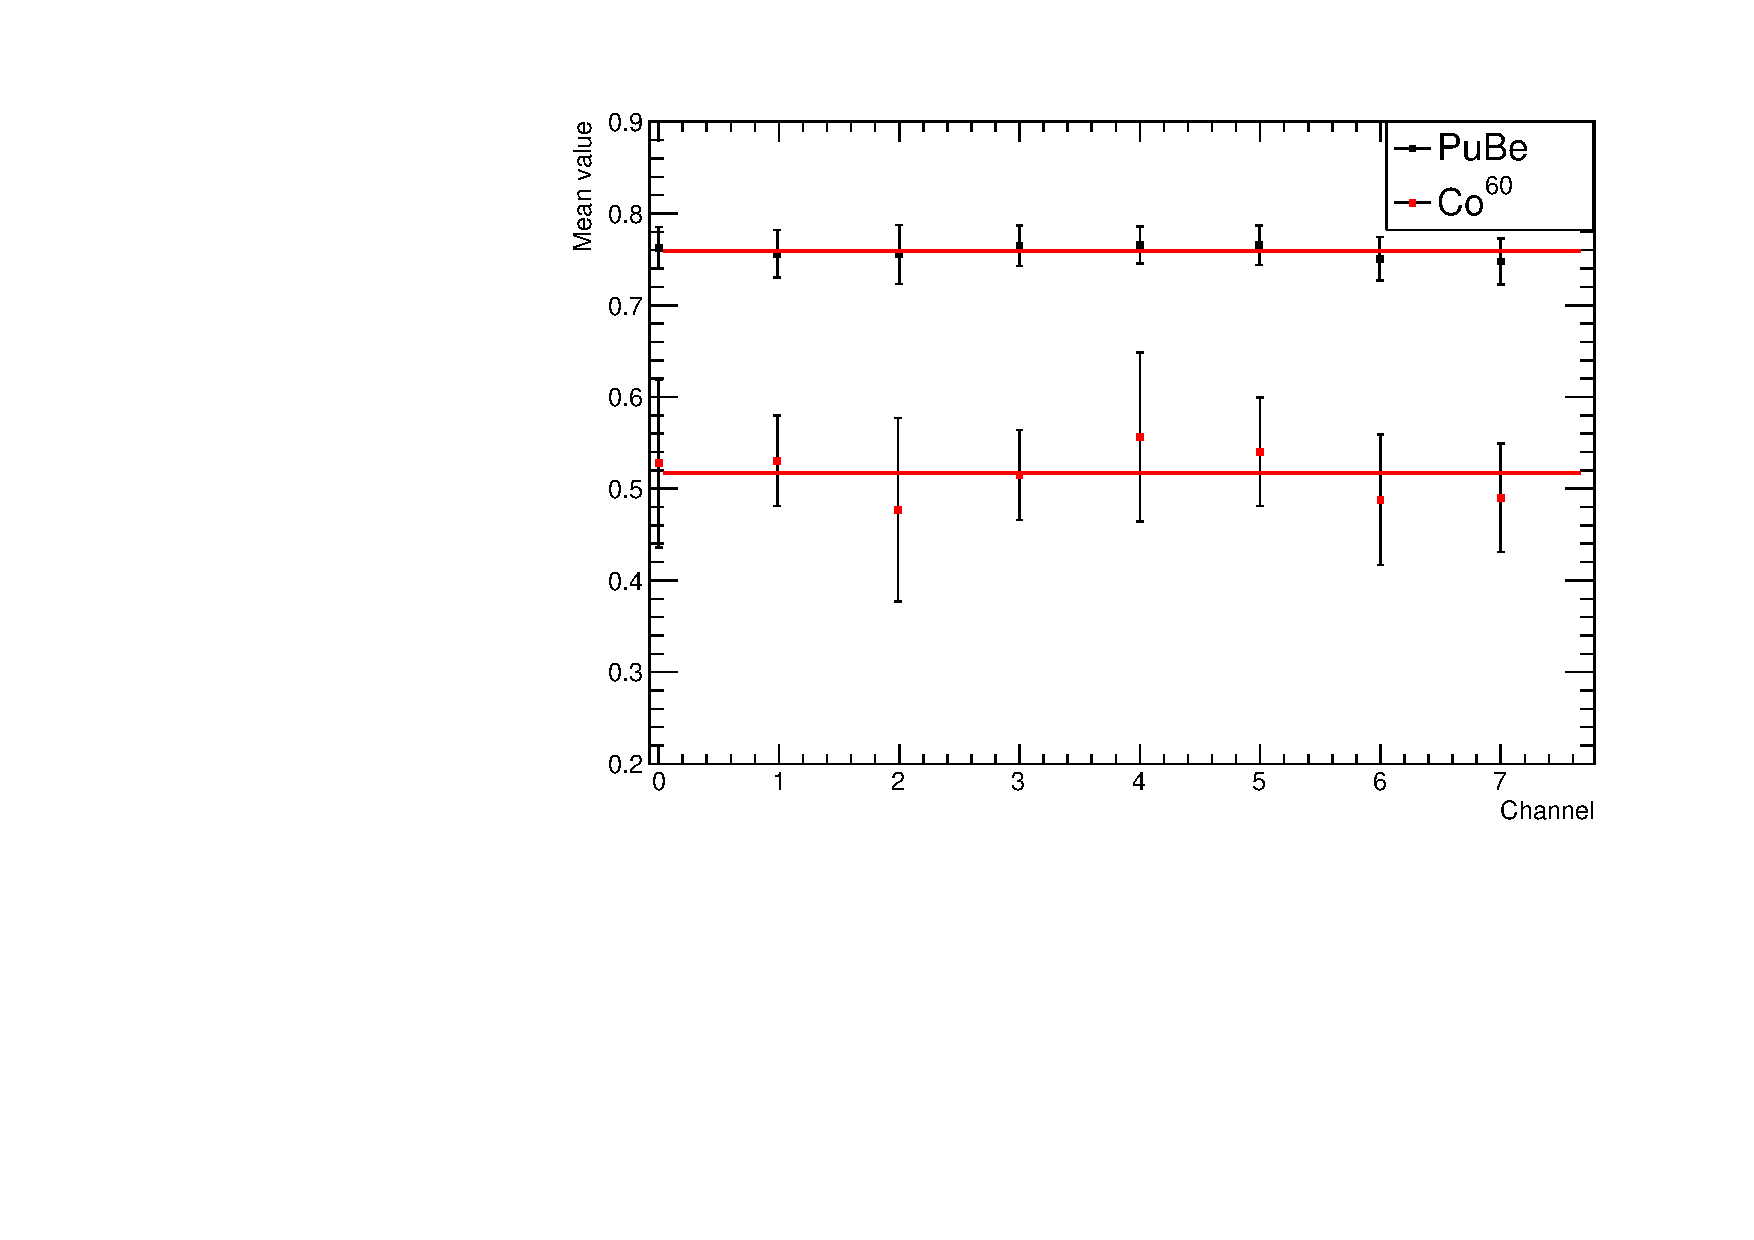
\includegraphics[width=120mm]{Chapter8/figures/pdsMeanValuesPerChannel_SigmaErrors_withFit.pdf}
\caption{The mean values obtained from the Gaussian fit to the peak of the PSD distributions for each channel. The error bars represent $\pm$ 1$\sigma$ values from the fit. The red lines indicate the best fit value over all channels, 0.759 $\pm$ 0.008 and 0.52 $\pm$ 0.02 for PuBe and $^{60}$Co respectively. }
\label{fig:modesPSDMeanForChannels}
\end{center}
\end{figure}

To achieve an analysis that uses data collected from all/multiple channels, it is best to treat each channel/detector independently when optimising the selection for n-$\gamma$ discrimination. This can be seen in figure \ref{fig:modesEffAndPurAllChannels} which shows the efficiencies, purities and figure of merits varying for each channel also. Establishing a n-$\gamma$ selection on a channel by channel basis we can then identify the particle and combination of the rates can occur after selection. Due to non-linear effects it is not possible to calibrate each channel by shifting channel peaks to a common value without greater understanding and information on the detector conditions, the data acquired is insufficient. The best figure of merits values are shown in table \ref{tab:modesPSDAllChannelsBestFOMValues} along with their associated PSD selection values.

\begin{figure}[htbp]
\begin{center}
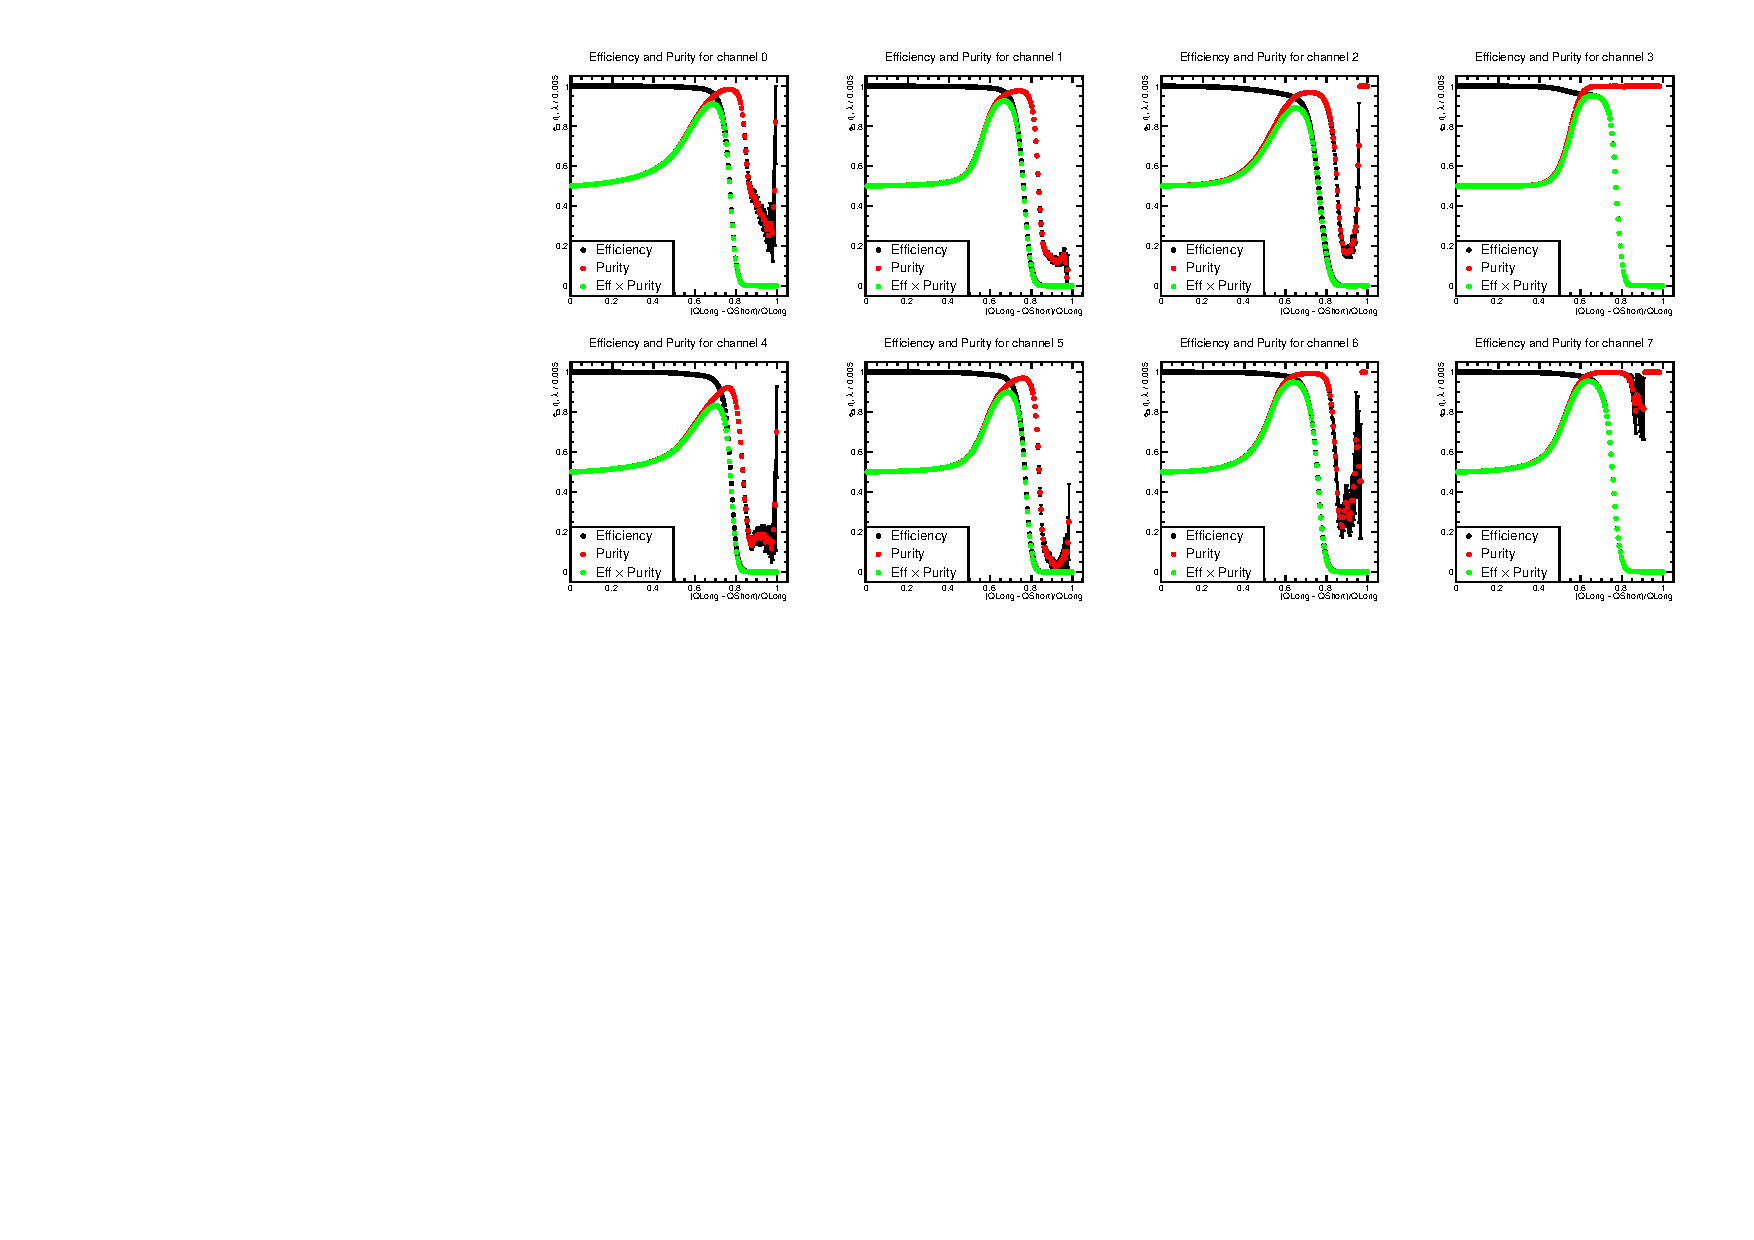
\includegraphics[width=160mm]{Chapter8/figures/eff_pur_allChannels_pube_co60_matchedEvents.pdf}
\caption{The efficiencies, purities and figure of merits comparing a neutron source, PuBe, with gamma source $^{60}$Co, for 8 channels across 4 fast neutron detectors. }
\label{fig:modesEffAndPurAllChannels}
\end{center}
\end{figure}

% Why is the neutron source narrower??? - Has much smaller short component of scintillation light? - Is Qshort the charge from the short gate or from the slow component???

\begin{table}[h]
\centering
	\begin{tabular}{ccc}
	\hline
	\textbf{Channel} & \textbf{Highest figure of merit value} ($\mathbf{\lambda_{max}}$)&  \textbf{PSD Selection value}\\
	\hline
	0  & 0.9117 $\pm$ 0.0006 & 0.695 $\pm$ 0.005 \\ 
	1  & 0.9260 $\pm$ 0.0006 & 0.675 $\pm$ 0.005 \\ 
	2  & 0.8910 $\pm$ 0.0020 & 0.655 $\pm$ 0.005 \\ 
	3  & 0.9514 $\pm$ 0.0009 & 0.655 $\pm$ 0.005 \\ 
	4  & 0.8327 $\pm$ 0.0009 & 0.705 $\pm$ 0.005 \\ 
	5  & 0.8999 $\pm$ 0.0009 & 0.695 $\pm$ 0.005 \\ 
	6  & 0.9500 $\pm$ 0.0010 & 0.645 $\pm$ 0.005 \\ 
	7  & 0.9550 $\pm$ 0.0010 & 0.645 $\pm$ 0.005 \\ 
	\hline
\end{tabular}
\caption{A table showing the highest achieved figure of merit values, $\lambda_{max}$, when optimising the PSD selection on a channel basis. }
\label{tab:modesPSDAllChannelsBestFOMValues}
\end{table}

\subsubsection{Improving the Selection}
Examining the maximum figure of merit values, $\lambda_{max}$, from table \ref{tab:modesPSDAllChannelsBestFOMValues} there is large variation between the channels with the lowest value at 0.8327 $\pm$ 0.0009 and the highest value reaching 0.9550 $\pm$ 0.0010. With the figure of merit a strong indicator of detection efficiency and purity, even at this highest value the efficiencies would be far below the limit imposed on the detector requirements. We propose to improve the figure of merit and hence the efficiencies for each channel via a method of sampling the collected data and measuring the PSD mean within the sample. Using the mean PSD value should then provide a more accurate PSD distribution for both neutrons and gamma sources which can then be used to establish a higher figure of merit. The algorithm can be summarised as the following:
\begin{enumerate}
	\item Select an appropriate average sample size - $\bar{n}$
	\item Get the number of events from the channel with the lowest number - $m_{min}$
	\item Establish the total number of experiments such that all channels have the same number of experiments - $N_{exp}$ = $m_{min}/\bar{n}$
	\item Establish a value for the sample size for each experiment based on the mean value from a Poisson distribution - $n$
	\item From the full data set of the channel take $n$ random events 
	\item Require the same sample size for both channels in the detector tube
	\item Calculate the mean of the PSD values for the channel
	\item Fill the mean PSD value in the appropriate bin in the histogram
	\item Increase the number of experiments performed
	\item Take a new sample - go to step 4
	\item Repeat until $N_{exp}$ is reached per channel
	\item Optimise n-$\gamma$ PSD selection based on maximising the figure of merit value	
\end{enumerate}


Taking an initial sample size of 100 events, results in a total of 80 experiments given the data samples for all channels and sources. Performing the analysis steps discussed above results in figure of merits of unity for all channels, with the PSD distributions shown in figure \ref{fig:modesPSDMean100EventsAllChannels} and the efficiencies, purities and figure of merits shown in figure \ref{fig:modesEffAndPurMean100EventsAllChannels}. However such a sample size would be unrealistic in real life deployment where much lower statistics are expected. To study the effect of the sample size on the PSD distributions and hence the figure of merit values, samples were reduced to sizes of 10, 8, 6, 4 and 2 events. The choice of these sizes were taken as $\lambda_{max}$ only began to drop below unity when the mean sample size dropped below 12 events  The best figure of merit values can be seen in figure \ref{fig:modesBestFOMDiffEventSamplesAllChannels} for each channel and for each of the different sample sizes.

\begin{figure}[htbp]
\begin{center}
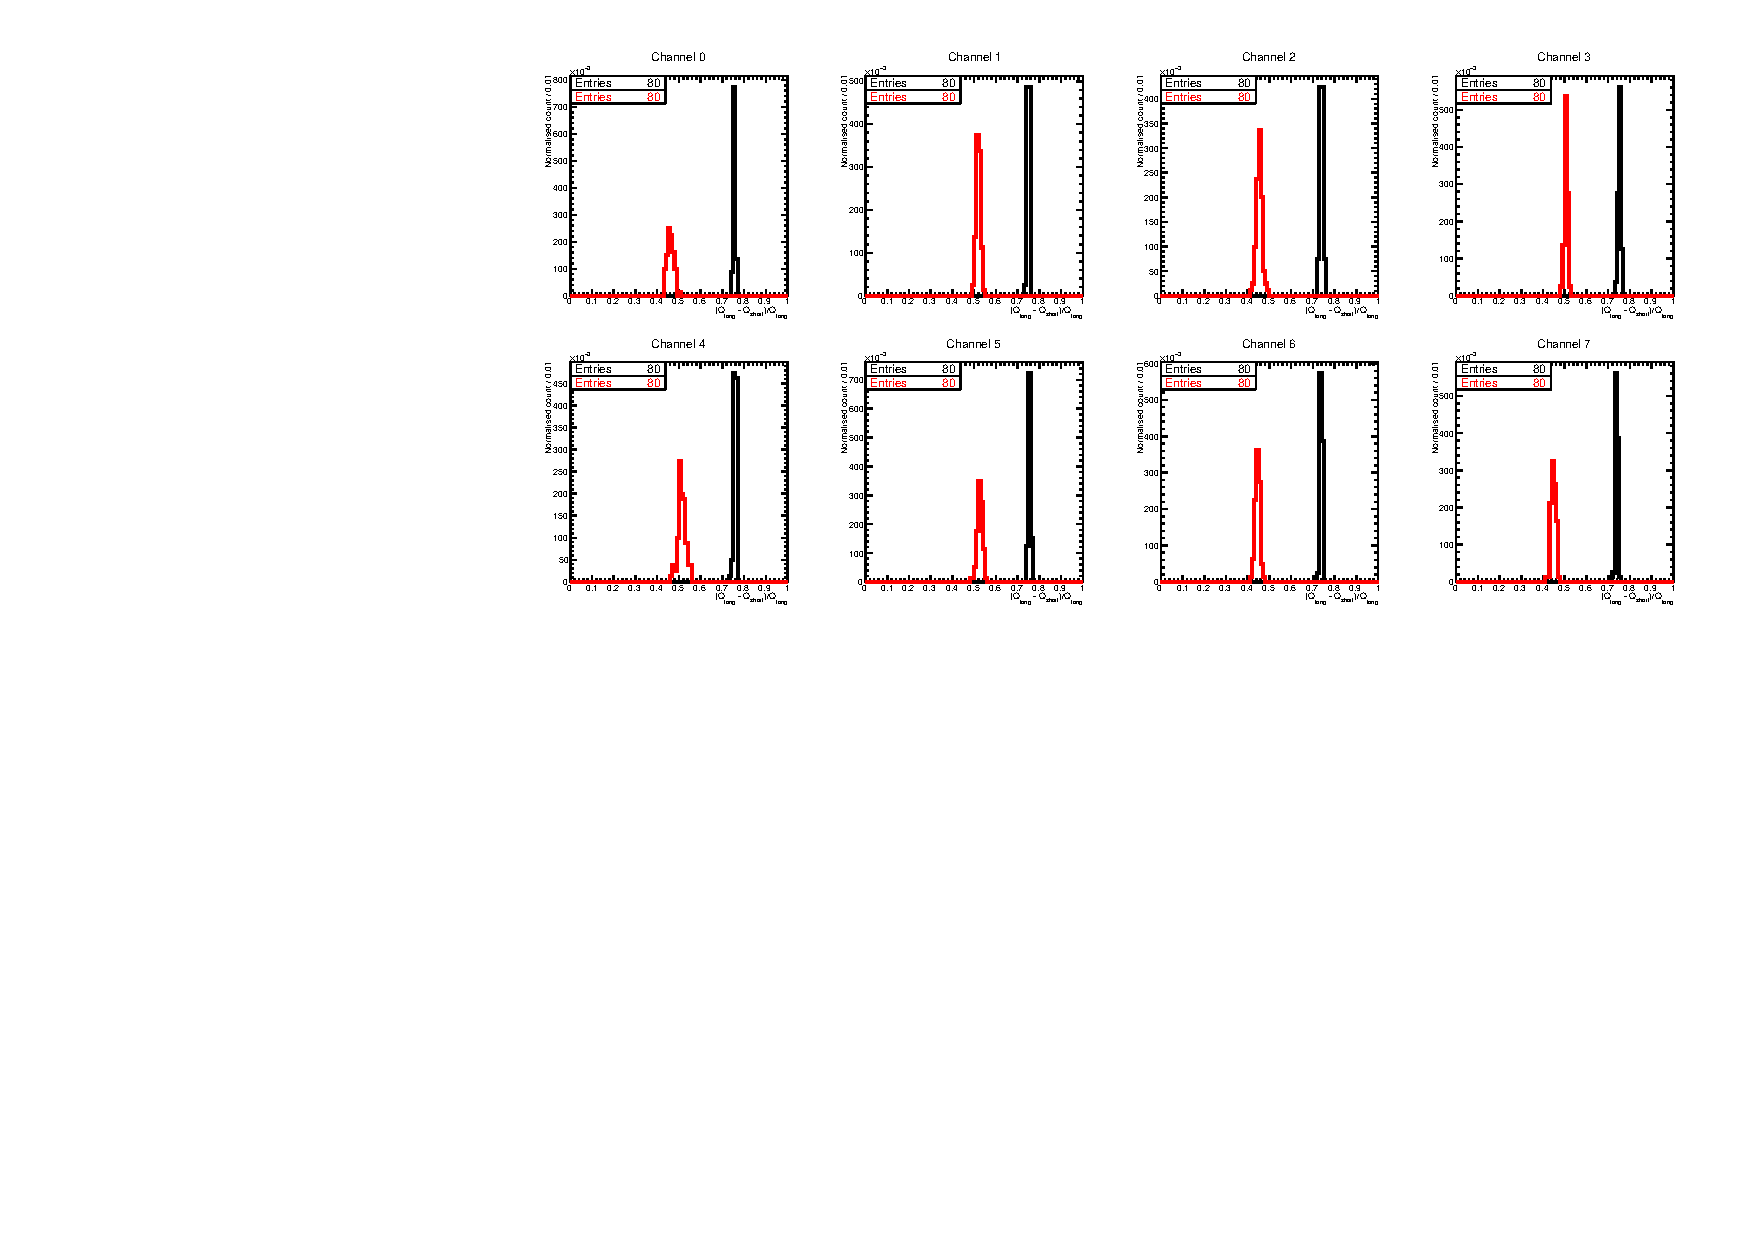
\includegraphics[width=160mm]{Chapter8/figures/psd_allChannels_pube_co60_mean100Events_80Experiments.pdf}
\caption{The mean PSD values binned in a histogram for a neutron source, PuBe (black), and a gamma source $^{60}$Co (red), for 8 channels across 4 fast neutron detectors. A sample size of 100 events were used with a total of 80 experiments performed over the data set.}
\label{fig:modesPSDMean100EventsAllChannels}
\end{center}
\end{figure}

\begin{figure}[htbp]
\begin{center}
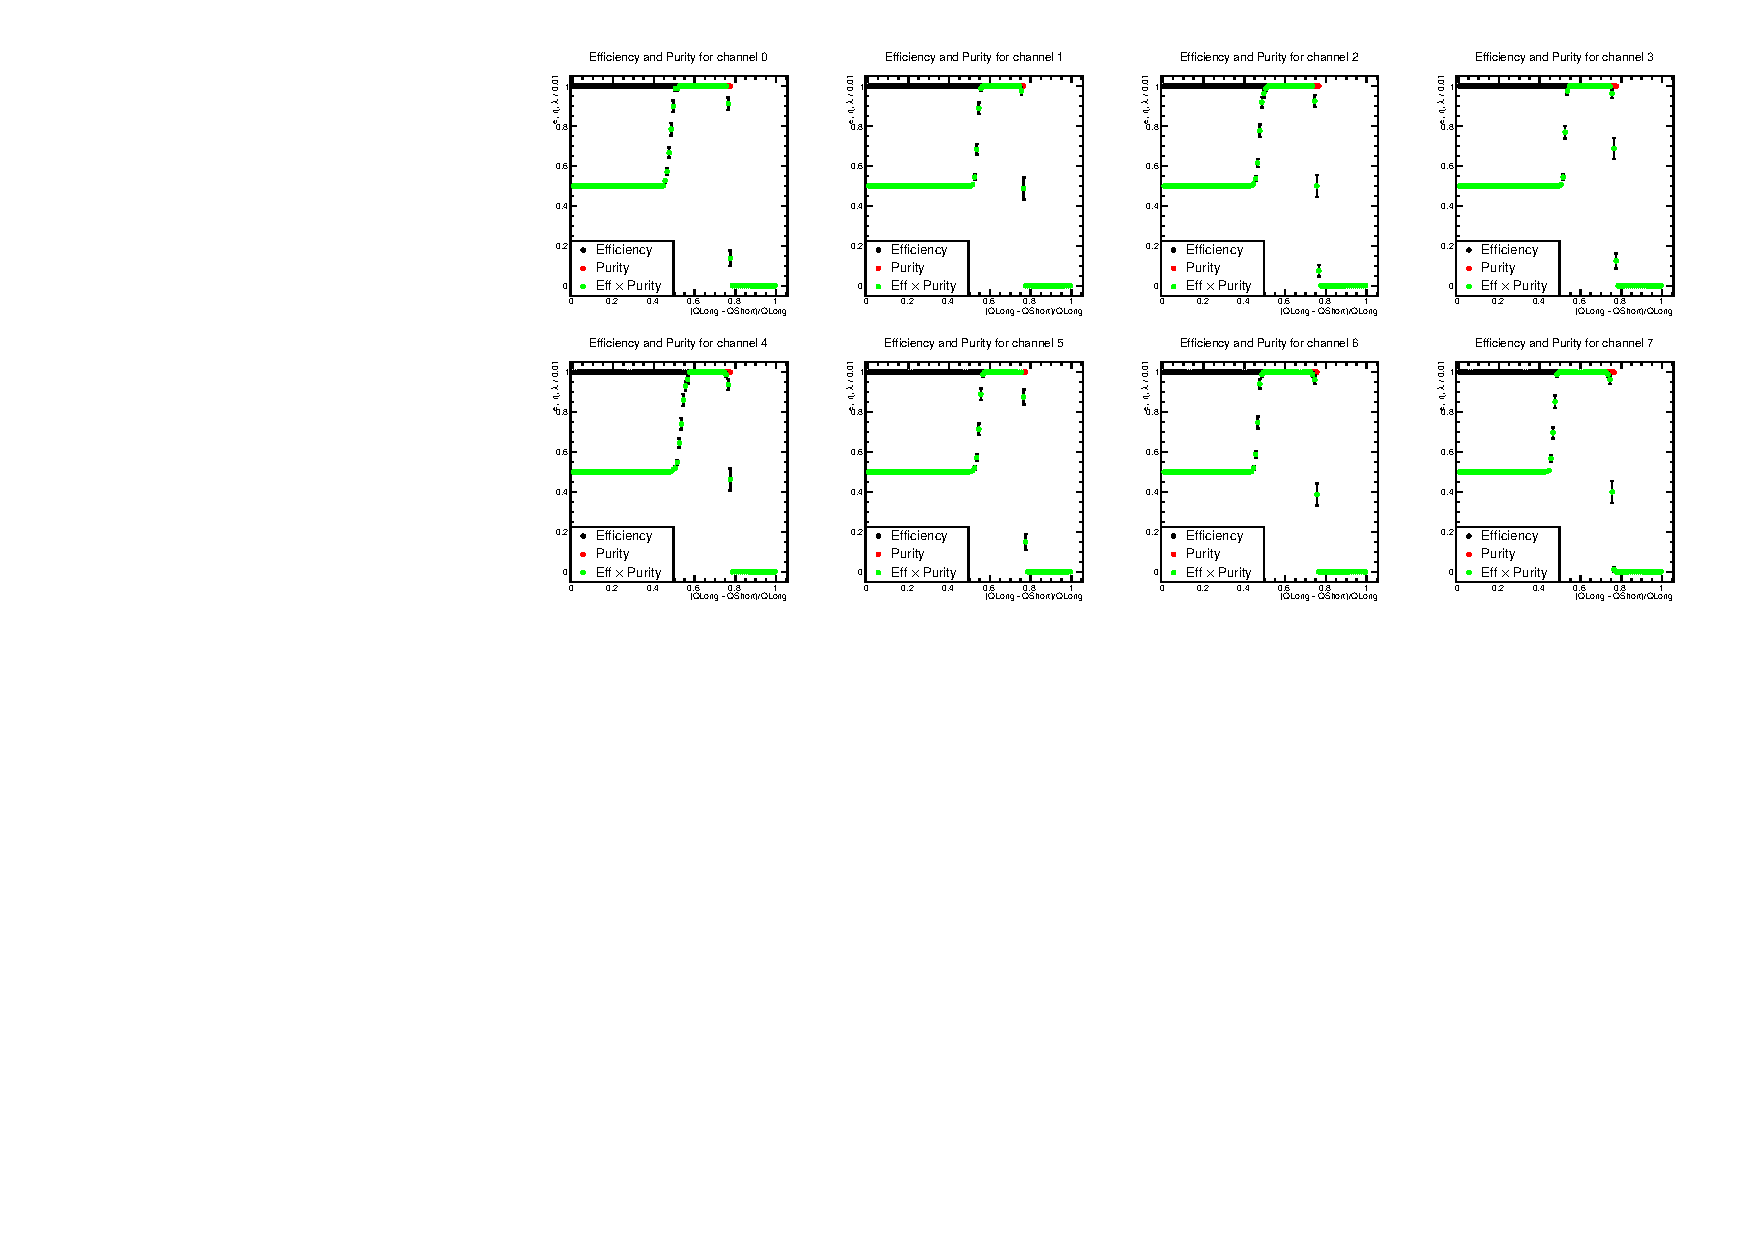
\includegraphics[width=160mm]{Chapter8/figures/eff_pur_allChannels_pube_co60_mean100Events_80Experiments.pdf}
\caption{The efficiencies, purities and figure of merits based on the mean PSD values for a sample size of 100 events with 80 experiments performed. The comparison is between a neutron source, PuBe, and a gamma source $^{60}$Co, for 8 channels across 4 fast neutron detectors.}
\label{fig:modesEffAndPurMean100EventsAllChannels}
\end{center}
\end{figure}

% This table represents the data used in the graph below.
%\begin{table}[h]
%\centering
%	\begin{tabular}{c|ccccc}
%	\hline
%	                           & \multicolumn{5}{c}{\textbf{Highest figure of merit value} ($\mathbf{\lambda_{max}}$)} \\
%				  & \textbf{10 events} & \textbf{8 events} & \textbf{6 events} & \textbf{4 events}& \textbf{2 events}\\
%         \textbf{Channel} & \textbf{857 exp} & \textbf{1099 exp} & \textbf{1431 exp} & \textbf{2113 exp}& \textbf{3734 exp}\\
%	\hline
%	0  & 1.000 $\pm$ 0.000 & 0.999 $\pm$ 0.001 & 0.992 $\pm$ 0.002 & 0.981 $\pm$ 0.003 & 0.959 $\pm$ 0.003\\ 
%	1  & 0.998 $\pm$ 0.002 & 0.998 $\pm$ 0.001 & 0.988 $\pm$ 0.003 & 0.983 $\pm$ 0.003 & 0.964 $\pm$ 0.003\\ 
%	2  & 0.996 $\pm$ 0.002 & 0.994 $\pm$ 0.002 & 0.981 $\pm$ 0.003 & 0.957 $\pm$ 0.004 & 0.925 $\pm$ 0.004\\ 
%	3  & 1.000 $\pm$ 0.000 & 1.000 $\pm$ 0.000 & 0.997 $\pm$ 0.002 & 0.991 $\pm$ 0.002 & 0.970 $\pm$ 0.003\\ 
%	4  & 0.999 $\pm$ 0.001 & 0.994 $\pm$ 0.002 & 0.981 $\pm$ 0.004 & 0.957 $\pm$ 0.004 & 0.906 $\pm$ 0.005\\ 
%	5  & 1.000 $\pm$ 0.000 & 0.997 $\pm$ 0.002 & 0.995 $\pm$ 0.002 & 0.976 $\pm$ 0.003 & 0.942 $\pm$ 0.004\\ 
%	6  & 1.000 $\pm$ 0.000 & 0.999 $\pm$ 0.001 & 0.997 $\pm$ 0.002 & 0.989 $\pm$ 0.002 & 0.965 $\pm$ 0.003\\ 
%	7  & 1.000 $\pm$ 0.000 & 1.000 $\pm$ 0.000 & 0.997 $\pm$ 0.002 & 0.988 $\pm$ 0.002 & 0.977 $\pm$ 0.002\\ 
%	\hline
%\end{tabular}
%\caption{A table showing the highest achieved figure of merit values, $\lambda_{max}$, when optimising the PSD selection on a channel basis. The figure of merit values are shown for sample sizes of 10, 8, 6, 4 and 2 events, along with their corresponding number of experiments.}
%\label{tab:modesPSDAllChannelsBestFOMValuesEventSamples}
%\end{table}

\begin{figure}[htbp]
\begin{center}
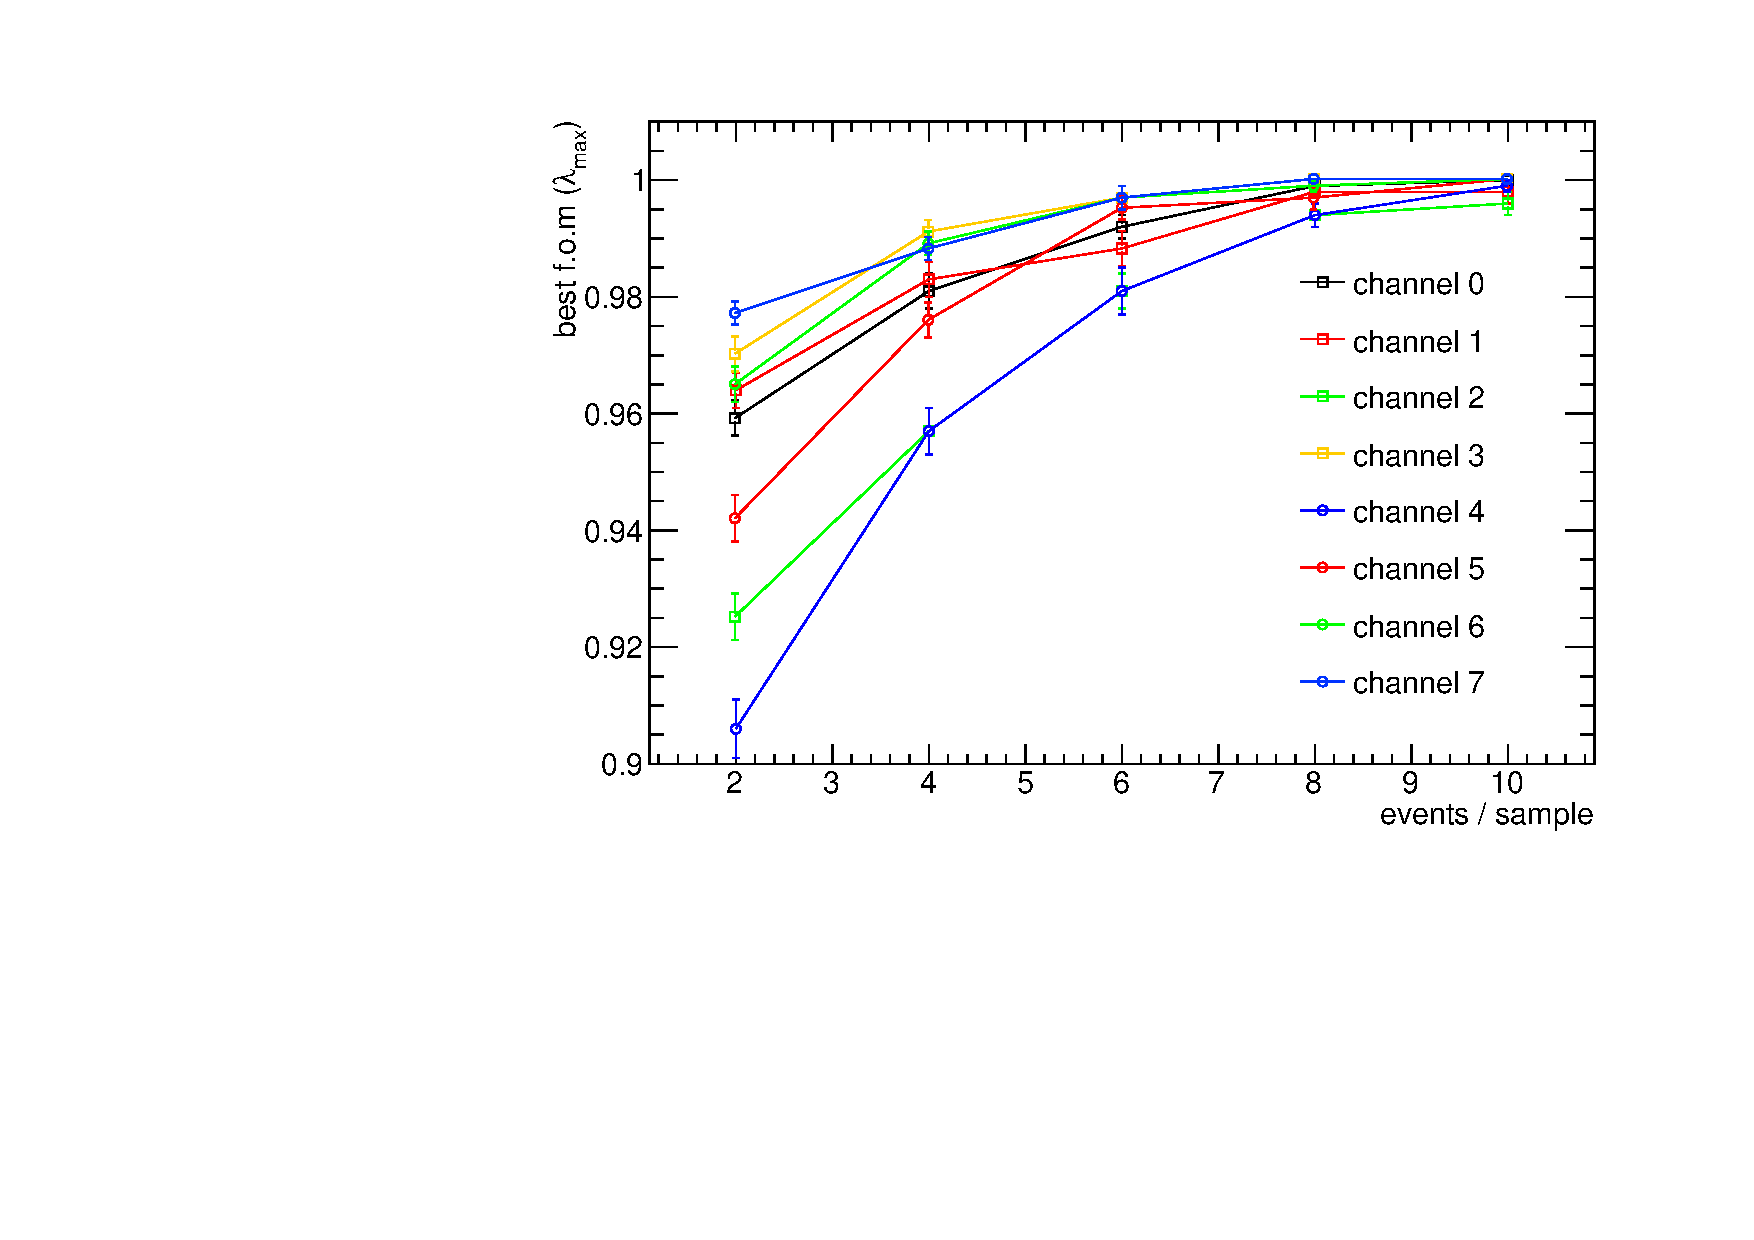
\includegraphics[width=160mm]{Chapter8/figures/allChannels_bestFOM_diffEventSamples.pdf}
\caption{The highest figure of merit values achieved, $\lambda_{max}$, when optimising the PSD selection on a channel basis. The values are shown for mean sample sizes of 10, 8, 6, 4 and 2 events, for all 8 channels. The number of experiments varied for each event sample size, with 3734, 2113, 1431, 1075 and 857 experiments for mean sample sizes of 2, 4, 6, 8 and 10 respectively.}
\label{fig:modesBestFOMDiffEventSamplesAllChannels}
\end{center}
\end{figure}

There is considerable variation between the figure of merit values over the channels at lower sample sizes with channel 4 reaching the lowest value at 0.906 $\pm$ 0.005. At this low sample size no channels figure of merit exceeded 0.98 but at the larger sample sizes of 8 and 10 the figure of merit is much improved with values exceeding 0.994 and with many channels at  $\lambda_{max}$ = 1. Although the figure of merit  takes both the efficiency and purity into account, such that the optimal PSD selection can be determined, the efficiency is the important parameter for particle discrimination. Taking the efficiencies at the optimal PSD selection, $\epsilon^{optimal}$, for each channel can then be used to define the total n-$\gamma$ discrimination efficiency for the 4 fast neutrons detectors combined. This will provide an insight to the expected efficiency of the full MODES-SNM system and hence we can determine if the false alarm rate is below the acceptable level. Simply, the n-$\gamma$ discrimination efficiency, $\epsilon_{tot}$, can be described by equation \ref{eq:modesTotSystemEff}. This then describes the number of neutrons that pass the cut, i.e. the number of neutrons that are detected as neutrons, for all channels combined. Since the number of experiments are used, denoted by $N_{i}$, is fixed for all channels and only varies depending on the sample size, $\epsilon_{tot}$ is simply equal to the average value across the channels. These values are shown for each mean sample size in table \ref{tab:modesPSDAllChannelsBestEffValuesEventSamplesNeutrons}.

\begin{equation}
\epsilon_{tot} = \frac{\sum^{ch=7}_{i=0}{N_{i}\epsilon^{optimal}_{i}}}{\sum^{ch=7}_{i=0}{N_{i}}} =\frac{1}{8}\sum^{ch=7}_{i=0}\epsilon^{optimal}_{i}
\label{eq:modesTotSystemEff}
\end{equation}

\begin{table}[h]
\centering
	\begin{tabular}{ccccc}
	\hline
	\hline
	\multicolumn{5}{c}{\textbf{Combined channel neutron detection efficiency}} \\
	\small{\textbf{10 events}} & \small{\textbf{8 events}} & \small{\textbf{6 events}} & \small{\textbf{4 events}}& \small{\textbf{2 events}}\\
        \small{\textbf{857 exp}} & \small{\textbf{1099 exp}} & \small{\textbf{1431 exp}} & \small{\textbf{2113 exp}}& \small{\textbf{3734 exp}}\\
	\hline
	 \small{0.9996 $\pm$ 0.0017} & \small{0.9980 $\pm$ 0.0036} & \small{0.9961 $\pm$ 0.0049} & \small{0.9891 $\pm$ 0.0064} & \small{0.9737 $\pm$ 0.0076}\\ 
	\hline
	\hline
\end{tabular}
\caption{A table showing the neutron detection efficiencies for 4 fast neutron detectors, combining all 8 channels. The efficiency values are shown for mean sample sizes of 10, 8, 6, 4 and 2 events, along with their corresponding number of experiments.}
\label{tab:modesPSDAllChannelsBestEffValuesEventSamplesNeutrons}
\end{table}

For all event sample sizes, we exceed the requirement of 96/100 neutron detection efficiency, with 10 mean events/sample reaching an efficiency of 0.9996 $\pm$ 0.0017 and 0.9737 $\pm$ 0.0076 for just 2 mean events/sample.

Similarly for misidentification alarms, we examine the number of $\gamma$'s that pass that selection, that is photons that are detected as neutrons. This is again determined in a similar fashion using equation \ref{eq:modesTotSystemEff} but now the efficiencies relate to $\gamma$'s that have a psd larger than the optimal selection, where 0 efficiency represents a 0 misidentification rate. Table \ref{tab:modesPSDAllChannelsBestEffValuesEventSamplesGammas} shows these rates. These values do not translate directly to false alarms, as a false alarm by definition is an alarm raised without explanation, that is when no source is present and the detectors are in a stable background. To translate these numbers to produce a estimate of the fast neutron detector false alarm rate we must first estimate an upper bound for the gamma background.

\begin{table}[h]
\centering
	\begin{tabular}{ccccc}
	\hline
	\hline
	\multicolumn{5}{c}{\textbf{Combined channel gamma misidentification efficiency}} \\
	\small{\textbf{10 events}} & \small{\textbf{8 events}} & \small{\textbf{6 events}} & \small{\textbf{4 events}}& \small{\textbf{2 events}}\\
        \small{\textbf{857 exp}} & \small{\textbf{1099 exp}} & \small{\textbf{1431 exp}} & \small{\textbf{2113 exp}}& \small{\textbf{3734 exp}}\\
	\hline
	 \small{0.0013 $\pm$ 0.0025} & \small{0.0022 $\pm$ 0.0034} & \small{0.0044 $\pm$ 0.0053} & \small{0.0120 $\pm$ 0.0110} & \small{0.0240 $\pm$ 0.0099}\\ 
	\hline
	\hline
\end{tabular}
\caption{A table showing the gamma misidentification detection efficiencies for 4 fast neutron detectors, combining all 8 channels. The efficiency values are shown for mean sample sizes of 10, 8, 6, 4 and 2 events, along with their corresponding number of experiments.}
\label{tab:modesPSDAllChannelsBestEffValuesEventSamplesGammas}
\end{table}

Due to the requirements set on the gamma detectors, a $^{60}$Co source of activity of $C$ = 160 kBq should be placed at a distance of $r$ = 1 m. Using this activity as the upper limit for an expected gamma background it can then be translated to an expected number of events across all 8 fast neutron detectors. In a $T$ = 2 second window, using equation \ref{eq:modesNrOfEventsGivenActivityRate} and detector parameters from table \ref{tab:neutronCfNumbers}, yields $\sim$87 gamma events. Note that a factor of two is used as $^{60}$Co produces 2 outgoing photons per disintegration (>99\% of the time) and the cross section on He$^{4}$, $\sigma_{\gamma \rightarrow He}$, is taken as a constant value of 0.01 m$^{2}$kg$^{-1}$, which is roughly valid between 0.1 to 1 MeV.

\begin{equation}
	N_{events} = \frac{8C\sigma_{\gamma \rightarrow He} \rho V_{0}T}{4\pi r^{2}}
	\label{eq:modesNrOfEventsGivenActivityRate}
\end{equation}

At this level of statistics, an average sample size of $\bar{n}$ = 100 would be unfeasible but $\bar{n}$ = 10 would, in this time frame to provide a enough experiments to perform the discrimination. However this would lead to a total of $\sim$20 false alarms per hour on average, much higher than permitted by the requirements. Given that $\lambda_{max}$ for mean sample sizes of $\sim$12 and above yield maximal efficiency and zero misidentification alarms for $^{60}$Co against PuBe, would provide remove all false alarms. To achieve mean samples sizes of 12, then we require at least 96 events across the 8 fast neutron detectors, which can be achieved in 3 s exposure.

%The misidentification rates were determined per channel not per detector, if done per detector/tube then can achieve higher value based on selecting the best figure of merit value. How in practice can we determine if it was a neutron or a gamma????
\subsubsection{Using the $^{137}$Cs Gamma Source}
Following the same procedure using a $^{137}$Cs gamma source requires larger mean sample sizes, $\bar{n}$ $\ge$ 50, to reach optimal $\lambda_{max}$ values across all channels. However the requirements for a $^{137}$Cs demand a larger activity of 660 kBq, 4.125 times larger than $^{60}$Co. At this activity this number of events can be achieved within a 3 s exposure at 1 m distance.

\subsubsection{Contamination Levels}
%To better understand how this analysis would perform in the presence of gamma
To emulate a real neutron source in the presence of a gamma background it is necessary to understand the effect of signal contamination on the efficiencies and purities. Signal contamination is the process of supplementing the neutron source (PuBe) with different levels of gamma ($^{60}$Co) events. 

Due to the requirements imposed on the system we can estimate the gamma background rate at the detectors. The minimum gamma dose rate for detection at 1 m distance is 0.05 $\mu$Sv/h, which is equivalent to a source of $\sim$160 kBq activity. This translates to a gamma flux at of $\phi_{\gamma}$ = 25.4 $\times$ 10$^{3}$ $\gamma$m$^{-2}$s$^{-1}$ at 1 m from the source, which is independent of whether the system is in stationary or mobile detection mode. If we define this value as the upper limit for the background rate then we can define the contamination rate relative to the neutron flux. 

The minimum neutron flux required for detection is defined as $\phi^{s}_{n}$ = 0.4 $\times$ 10$^{3}$ neutrons m$^{-2}$s$^{-1}$ and $\phi^{m}_{n}$ = 0.94 $\times$ 10$^{3}$ neutrons m$^{-2}$s$^{-1}$ for stationary and motion detection modes at 1 m from the source respectively. Considering the neutron and gamma peak emission is around 1 MeV we take a constant cross section for neutrons at 1 MeV of $\sigma_{n \rightarrow He}$ $\sim$0.2 m$^{2}$ kg$^{-1}$ and $\sigma_{\gamma \rightarrow He}$ $\sim$0.01 m$^{2}$ kg$^{-1}$ for $\gamma$'s at the same energy, as a rough estimate. Thus the ratio of cross sections is $\sigma_{n \rightarrow He}$/$\sigma_{\gamma \rightarrow He}$ $\sim$20. The $\gamma$ contamination level is then given by $\delta$ = $N_{\gamma}/(N_{n} + N_{\gamma})$ = $\phi_{n}\sigma_{n \rightarrow He} / (\phi_{n}\sigma_{n \rightarrow He} + \phi_{\gamma}\sigma_{\gamma \rightarrow He})$. For mobile neutron detection this corresponds to a level $\delta^{m}$ = 57.5\% gamma contamination with it increasing to $\delta^{s}$ = 76.0\% for stationary neutron detection. 

Through choice of an average sample size, $\bar{n}$, we establish the number of neutron events per experiment as $N_{n}= n - N_{\gamma}$, where both $n$ and $N_{\gamma}$ are taken from a Poisson distribution with mean values of $\bar{n}$ and $\bar{n}\delta$ respectively. Both $n$ and $N_{\gamma}$ are also determined per experiment, where the former represents the total number of contaminated events and the latter representing the number of gamma events for a signal experiment. Conversely the background experiments contain only gamma events, hence assuming a zero neutron contamination level. 

Taking $N_{n}$ events from the PuBe data set and $N_{\gamma}$ events from the $^{60}$Co data set per experiment, for 1 $\times$ 10$^{5}$ experiments, we then estimate the neutron detection efficiency and the gamma misidentification efficiencies as a function of the average number of contaminated events, $\bar{n}$. Both $N_{\gamma}$ and $N_{n}$ are determined on a tube basis, as the same number of neutrons and gammas interact within one tube, but PSD values are taken on a channel basis to avoid differences in channel parameters such as PMT voltage. Again all 8 channels are combined using equation \ref{eq:modesTotSystemEff}. The left of figure \ref{fig:modesContaminationEffVsEvents} shows the neutron detection efficiency as a function of $\bar{n}$ and with the right of figure \ref{fig:modesContaminationEffVsEvents} showing the misidentification efficiencies also a function of $\bar{n}$.

\begin{figure}[htbp]
\begin{center}
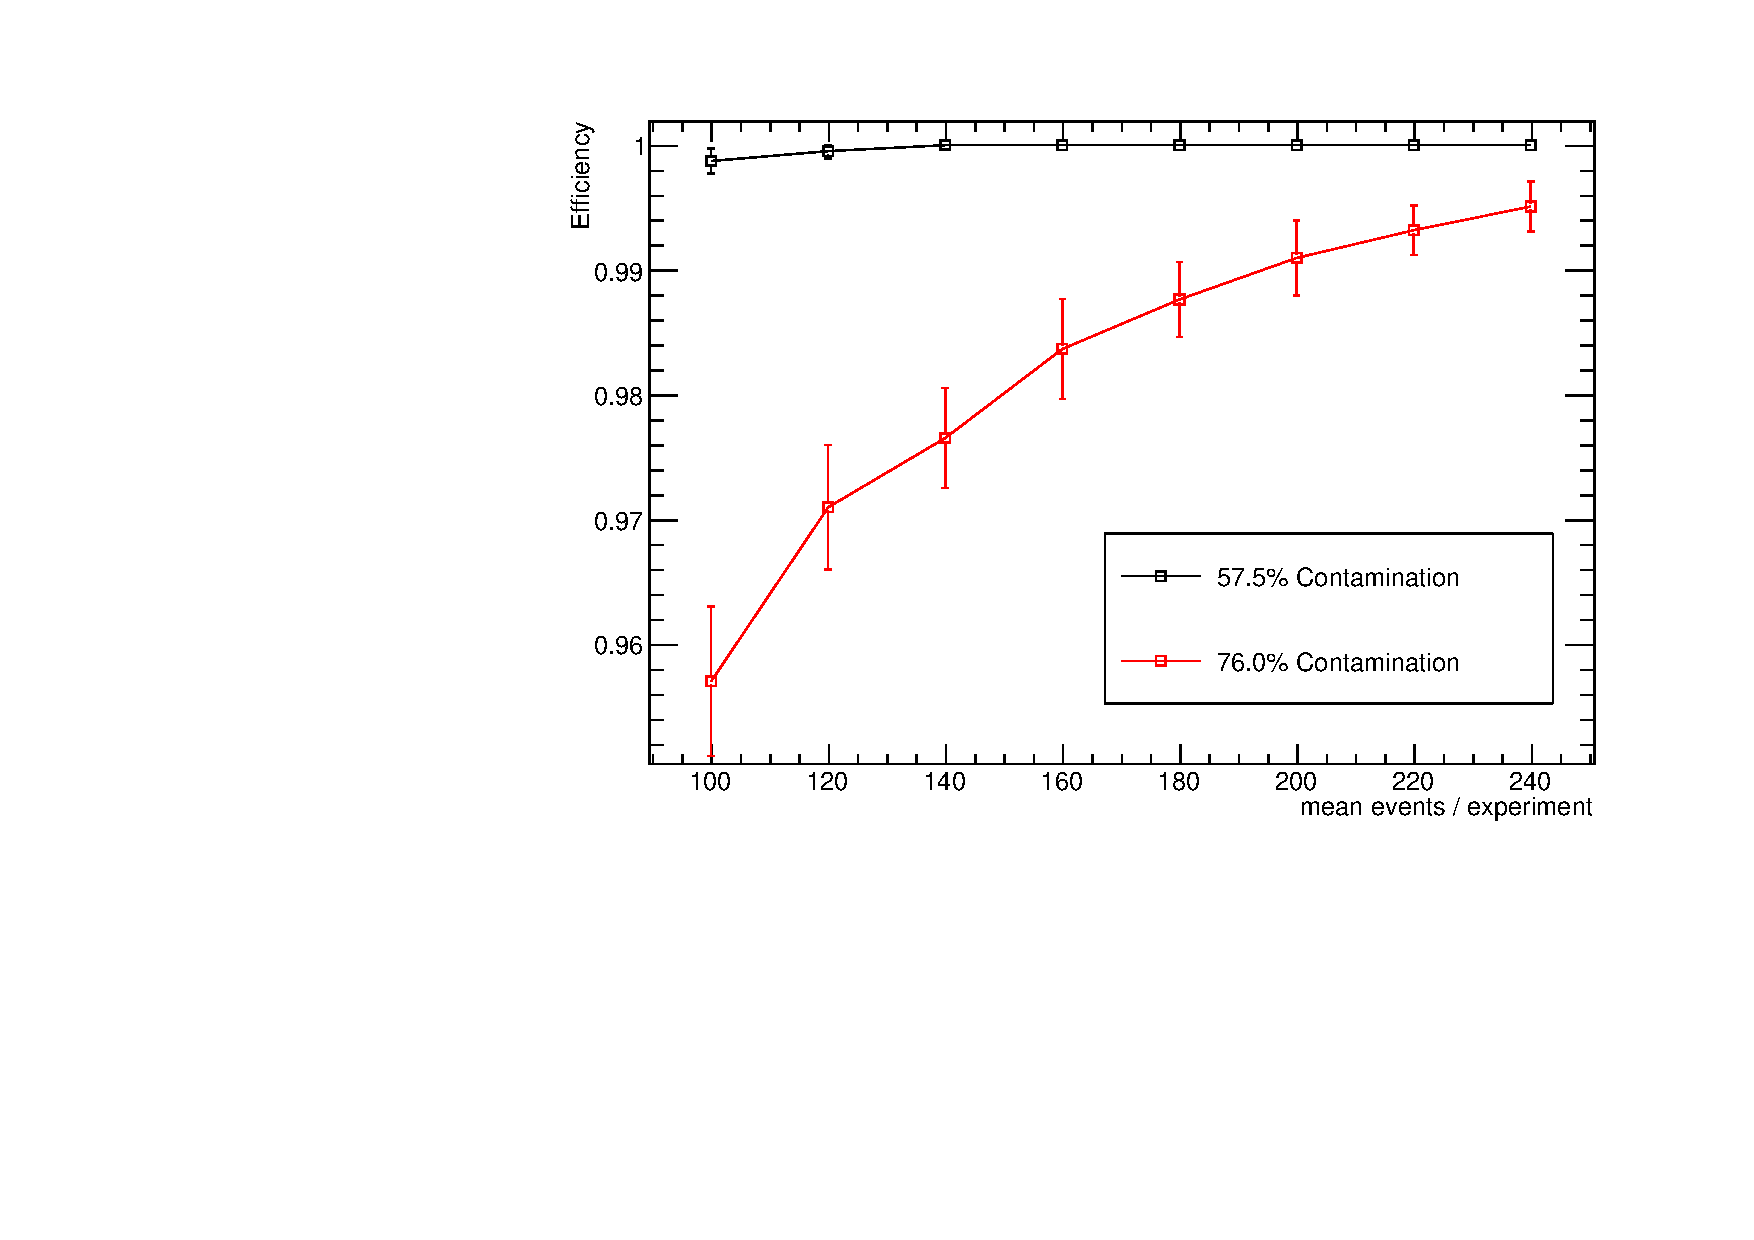
\includegraphics[width=74mm]{Chapter8/figures/efficiencySignal_contaminationLevel_vs_events.pdf}
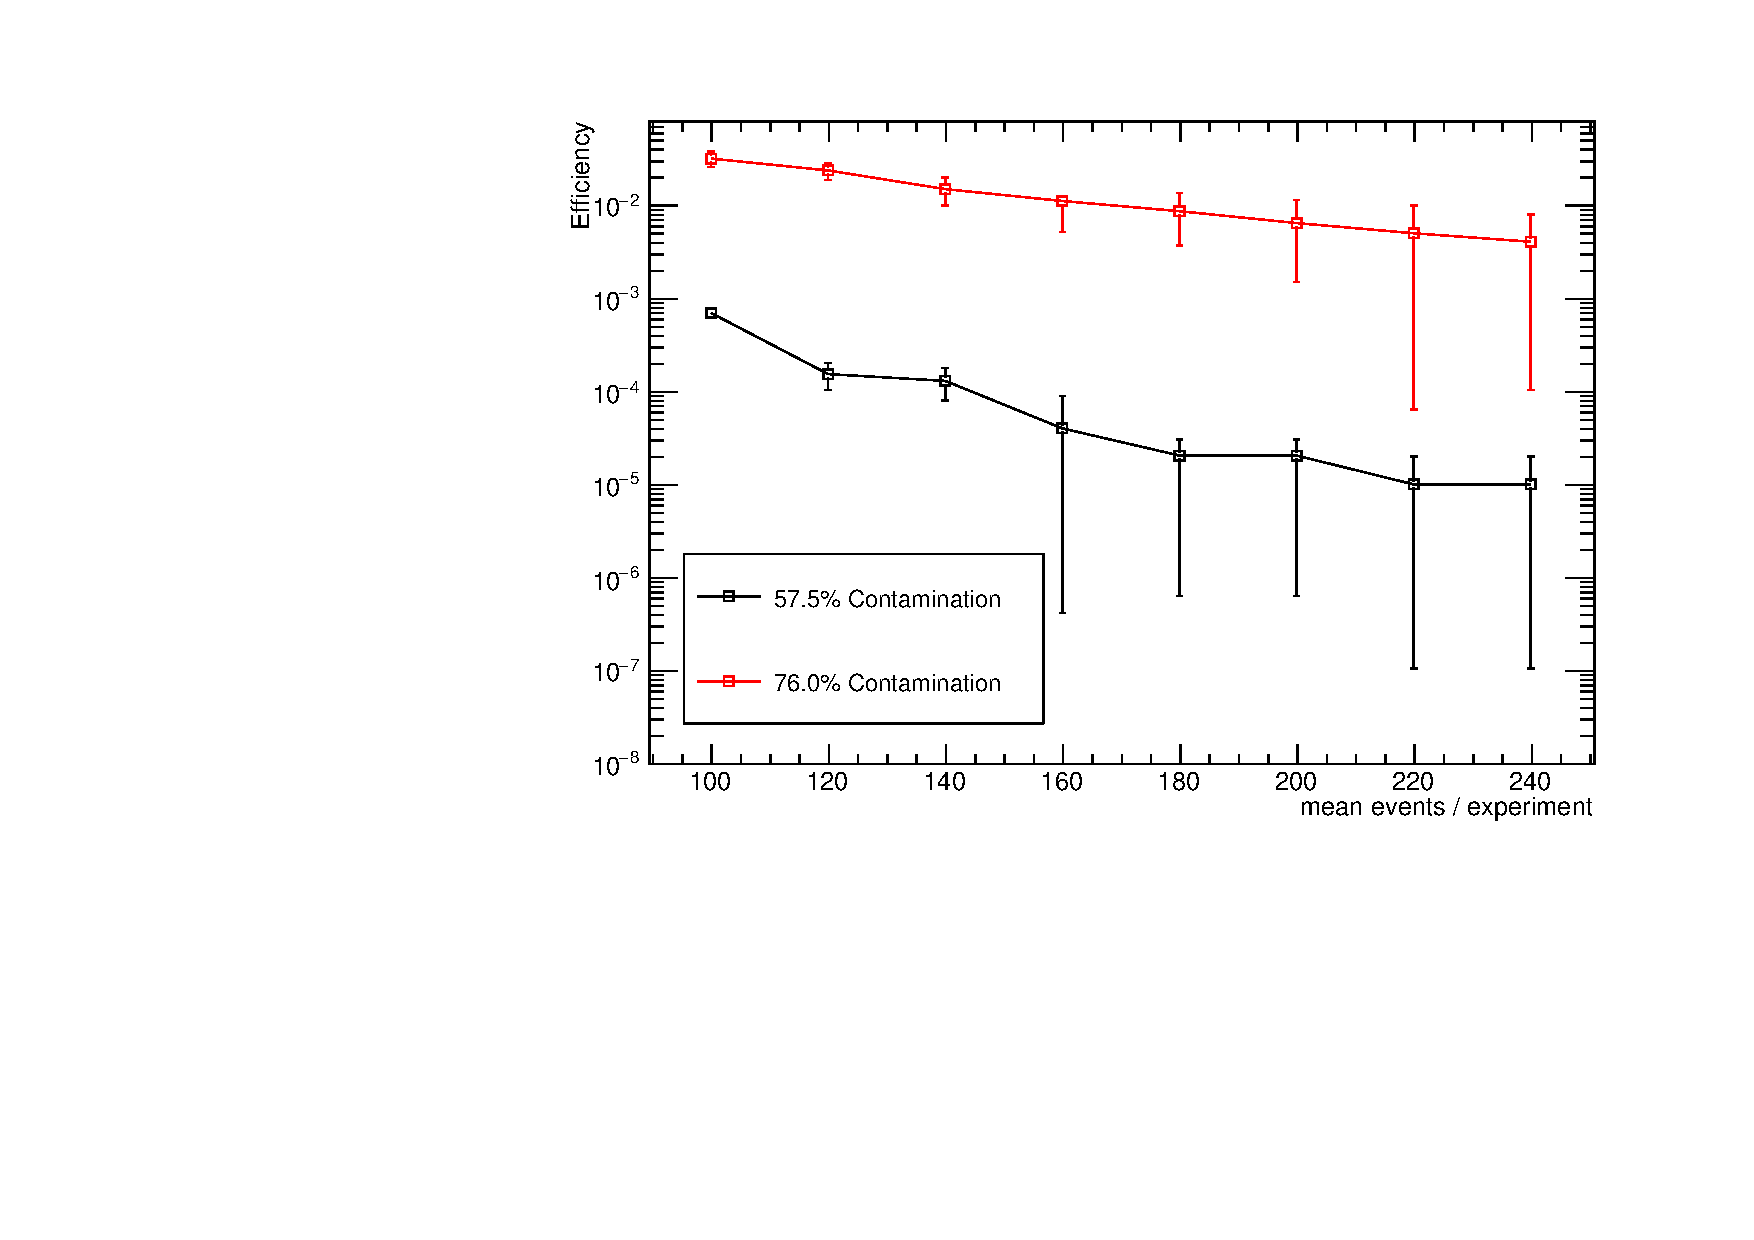
\includegraphics[width=74mm]{Chapter8/figures/misidentificationRate_contaminationLevel_vs_events.pdf}
\caption{Left: The neutron detection efficiencies as a function of the mean number of events per experiment. Right: The misidentification efficiencies as a function the mean number of events per experiment. Both show efficiencies for 57.5\% (black line) and 76.0\% (red line) levels of contamination corresponding to motion and stationary detection modes respectively.}
\label{fig:modesContaminationEffVsEvents}
\end{center}
\end{figure}

At a 2 second exposure we can expect to achieve $\bar{n}^{s}$ $\sim$116 and $\bar{n}^{m}$ $\sim$154 for stationary and motion detection modes respectively. For a 3 second exposure these increase to $\bar{n}^{s}$ $\sim$174 and $\bar{n}^{m}$ $\sim$231. Since motion detection has a lower contamination level it therefore achieves better efficiencies and yields higher statistics when compared to the stationary detection mode. For motion detection at a 3 second exposure we can expect to achieve a neutron detection efficiency of $\epsilon_{sig}$ = 1.00000 $\pm$ 0.00001 with a misidentification efficiency of $\epsilon_{bkg}$ = (1.0 $\pm$ 0.1 $\times$) 10$^{-5}$. Although the impact of reducing the exposure to 2 seconds only slightly reduces the efficiencies to $\epsilon_{sig}$ = 0.9999$^{+ 0.0001}_{-0.0003}$ and $\epsilon_{bkg}$ = (1.5 $\pm$ 0.1) $\times$ 10$^{-5}$. For stationary detection however the efficiencies are worse with $\epsilon_{sig}$ = 0.988 $\pm$ 0.003 and $\epsilon_{bkg}$ = 0.009 $\pm$ 0.004 for a 3 second exposure, with $\epsilon_{sig}$ = 0.967 $\pm$ 0.005 and $\epsilon_{bkg}$ = 0.023 $\pm$ 0.006 for a 2 second exposure. 

Due to requirements imposed on the system, the false alarm rate should not exceed 1 per hour, we can estimate how this translates to the misidentification efficiencies. We assume that per period of exposure of $T$ seconds, $\bar{n}$ events are accumulated, which then translates to 1 experiment. The resultant PSD value of this 1 experiment will then either pass or fail the PSD selection, hence we have $k$ = 60$^{2}\epsilon_{bkg}/T$, false alarms in one hour due to $\gamma$'s misidentified as neutrons. For motion detection this equates to 0.012 $\pm$ 0.001 and 0.027 $\pm$ 0.002 false neutron alarms per hour for 3 and 2 second exposures respectively. However for stationary detection we exceed the required rate with much higher rate of 11 $\pm$ 5 and 41 $\pm$ 11 false neutron alarms per hour for 3 and 2 second exposures respectively. Although for stationary detection the exposure period can well exceed 2/3 s periods and so higher statistics and better efficiencies can be achieved. Increasing the period to $T$= 6 s, $\epsilon_{bkg}$ is reduced to 0.0010 $\pm$ 0.0005, which then passes the requirement by achieving a false alarm rate of 0.6 $\pm$ 0.3 per hour.

We can conclude that the presented analysis demonstrates that n-$\gamma$ discrimination can be performed with the MODES-SNM system while maintaining the imposed detector requirements. Although these conclusions have been drawn from using a single $^{60}$Co source, the analysis has been formed in such a way as to make it independent of the source, given that other $\gamma$ sources with similar energy spectra could be used to produce similar results. However some assumptions have been made in the process with the approximations used on the expected number of interactions based on estimates of source activities. The corresponding activity of $^{60}$Co was used as the upper background estimation, given that the minimum gamma detection should be 0.05/h $\mu$Sv at 1 m from the source. This activity would translate differently for other similar gamma sources and it would be interesting to perform a similar analysis on sources such as $^{137}$Cs and $^{241}$Am to examine if the results still hold. A limiting factor on the analysis was the amount of data provided, given that I was not present for data collection and time was heavily restricted for testing. It must also be noted that these results are based on only 4 out of the possible 8 fast neutron detectors and it would of been also interesting to study the different effects of the detector array arrangement. 

%Only prototype, limited amount of time with the detector

